\chapter{Selection Binning}\label{appendix:bintemplates}

Templates for the non-uniform fit binning for each sample are presented in this section, as it is not feasible to express the bin edges in text for non-uniform binning. Figure \ref{fig:th2polybinreset5000} shows the x-axis range reduced to 0-5000 MeV so that the smaller bins in the peak can be seen. Figure \ref{fig:th2polybinreset} shows the full distributions out to 30 GeV, for each sample.

\begin{figure}
\centering
\begin{subfigure}{.32\textwidth}
  \centering
  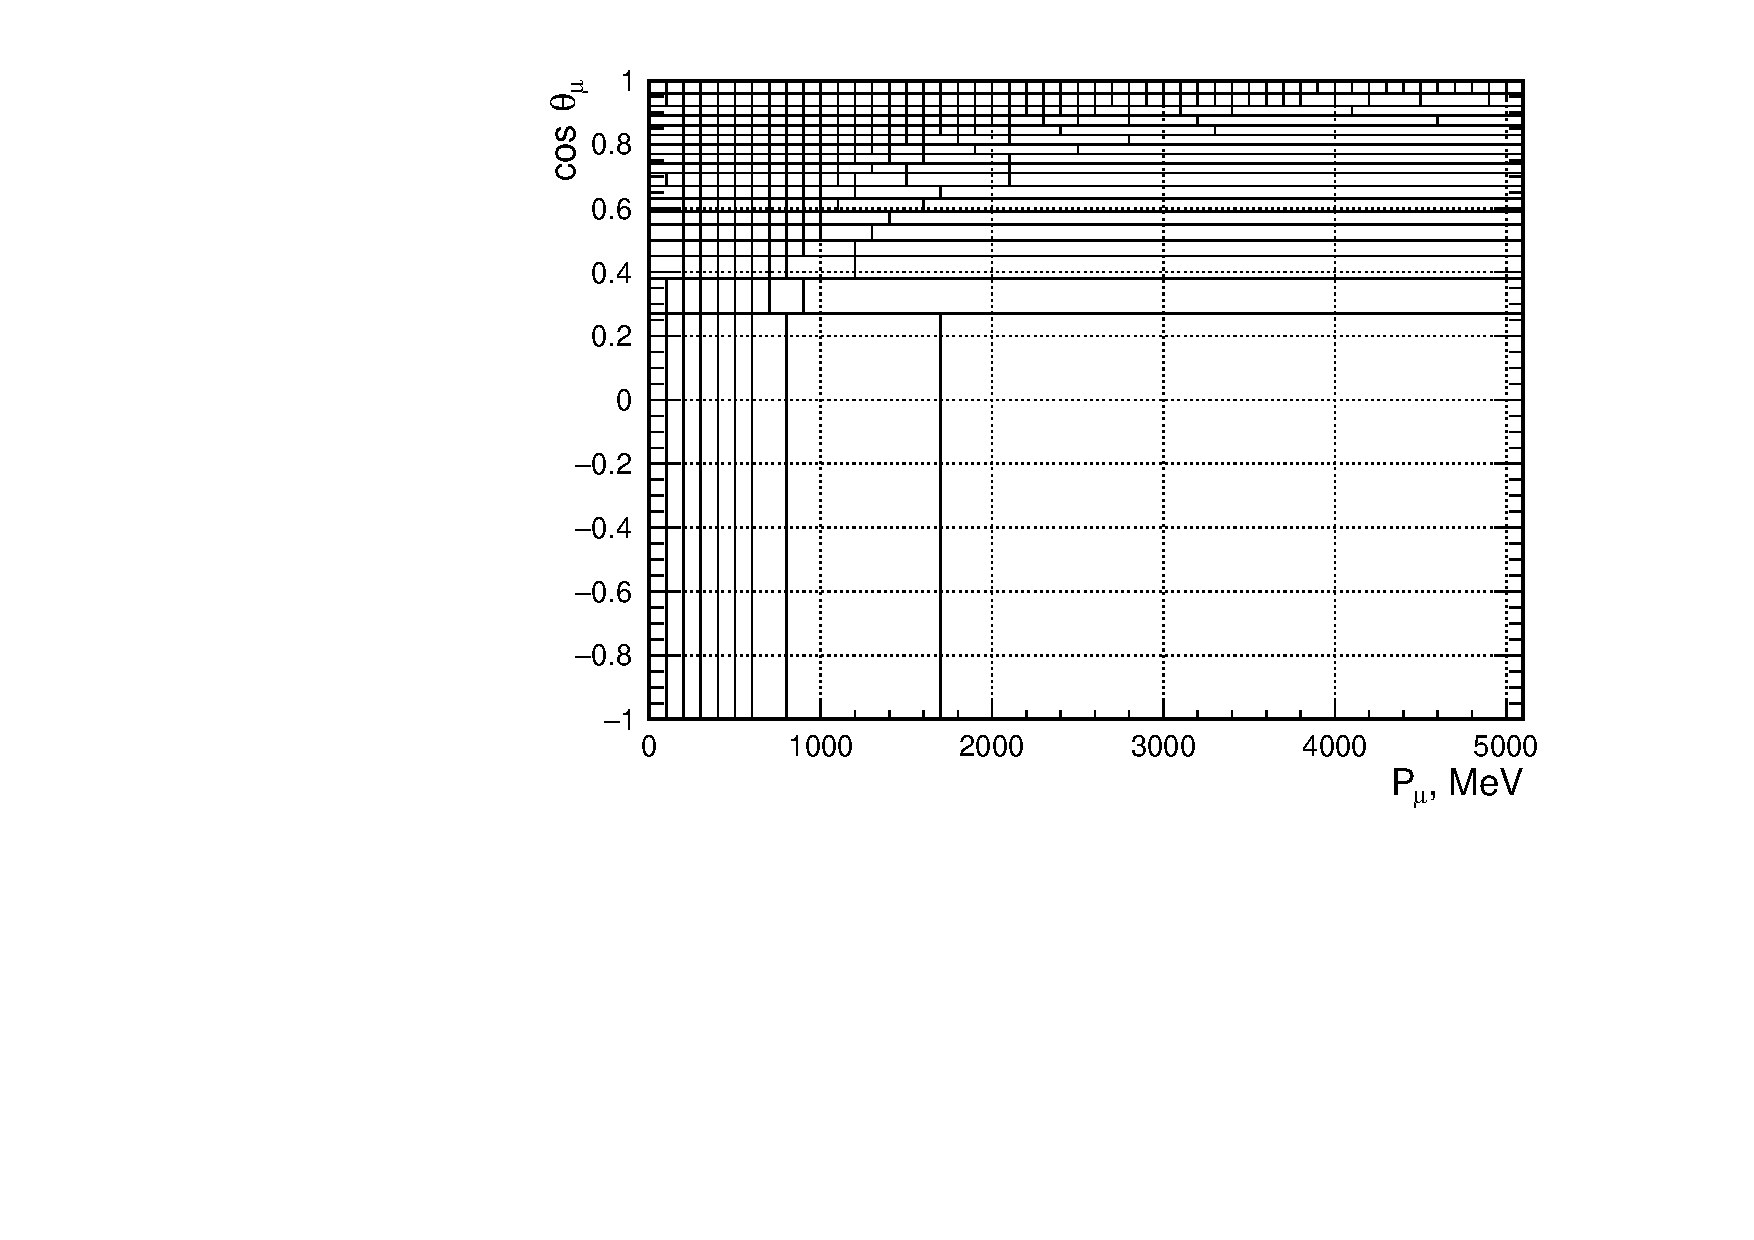
\includegraphics[width=0.95\linewidth]{figs/TH2PolyReset5000_MC_FGD1_numuCC_0pi}
  \caption{FGD1 FHC $\nu_{\mu}$ 0$\pi$}
  \label{fig:TH2Poly_Reset5000FGD1_numuCC_0pi}
\end{subfigure}
\begin{subfigure}{.32\textwidth}
  \centering
  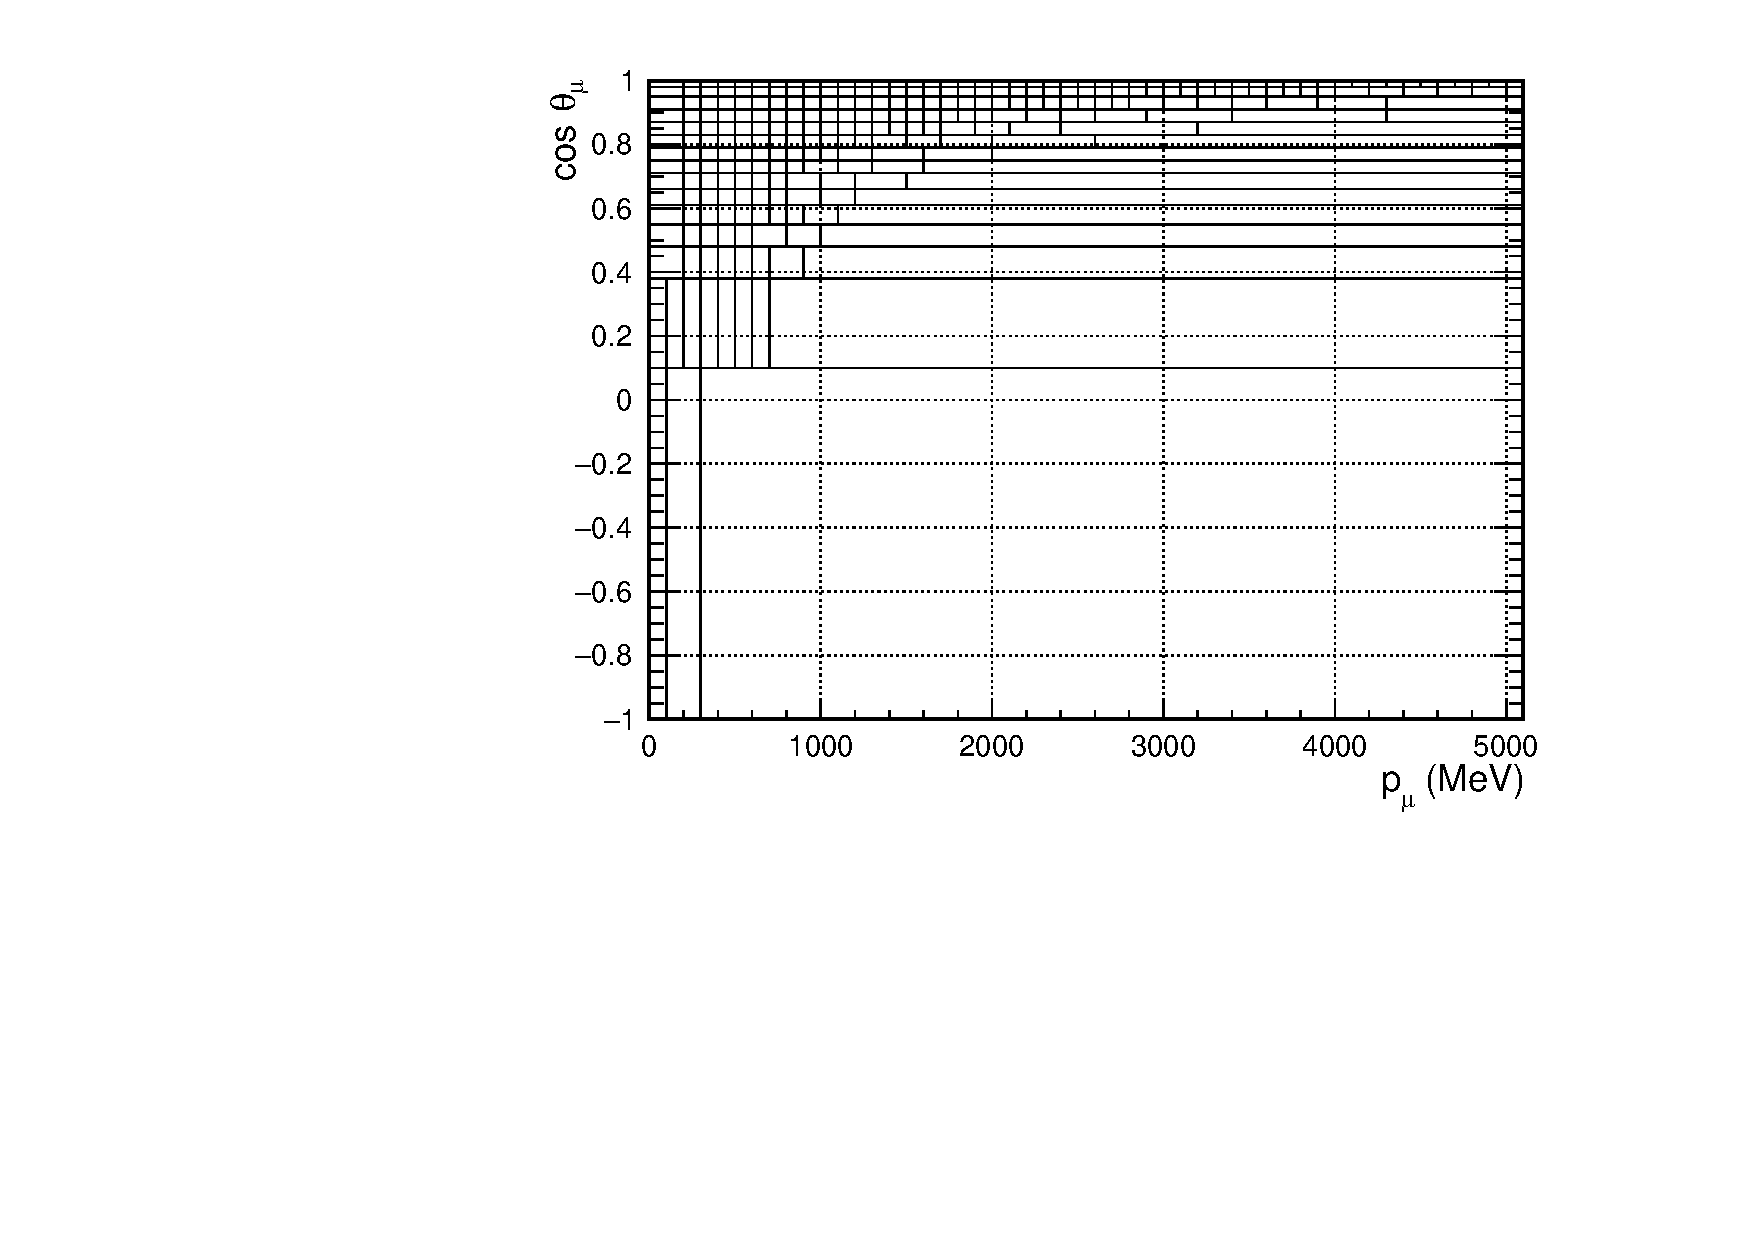
\includegraphics[width=0.95\linewidth]{figs/TH2PolyReset5000_MC_FGD1_numuCC_1pi}
  \caption{FGD1 FHC $\nu_{\mu}$ 1$\pi$}
  \label{fig:TH2Poly_Reset5000FGD1_numuCC_1pi}
\end{subfigure}
\begin{subfigure}{.32\textwidth}
  \centering
  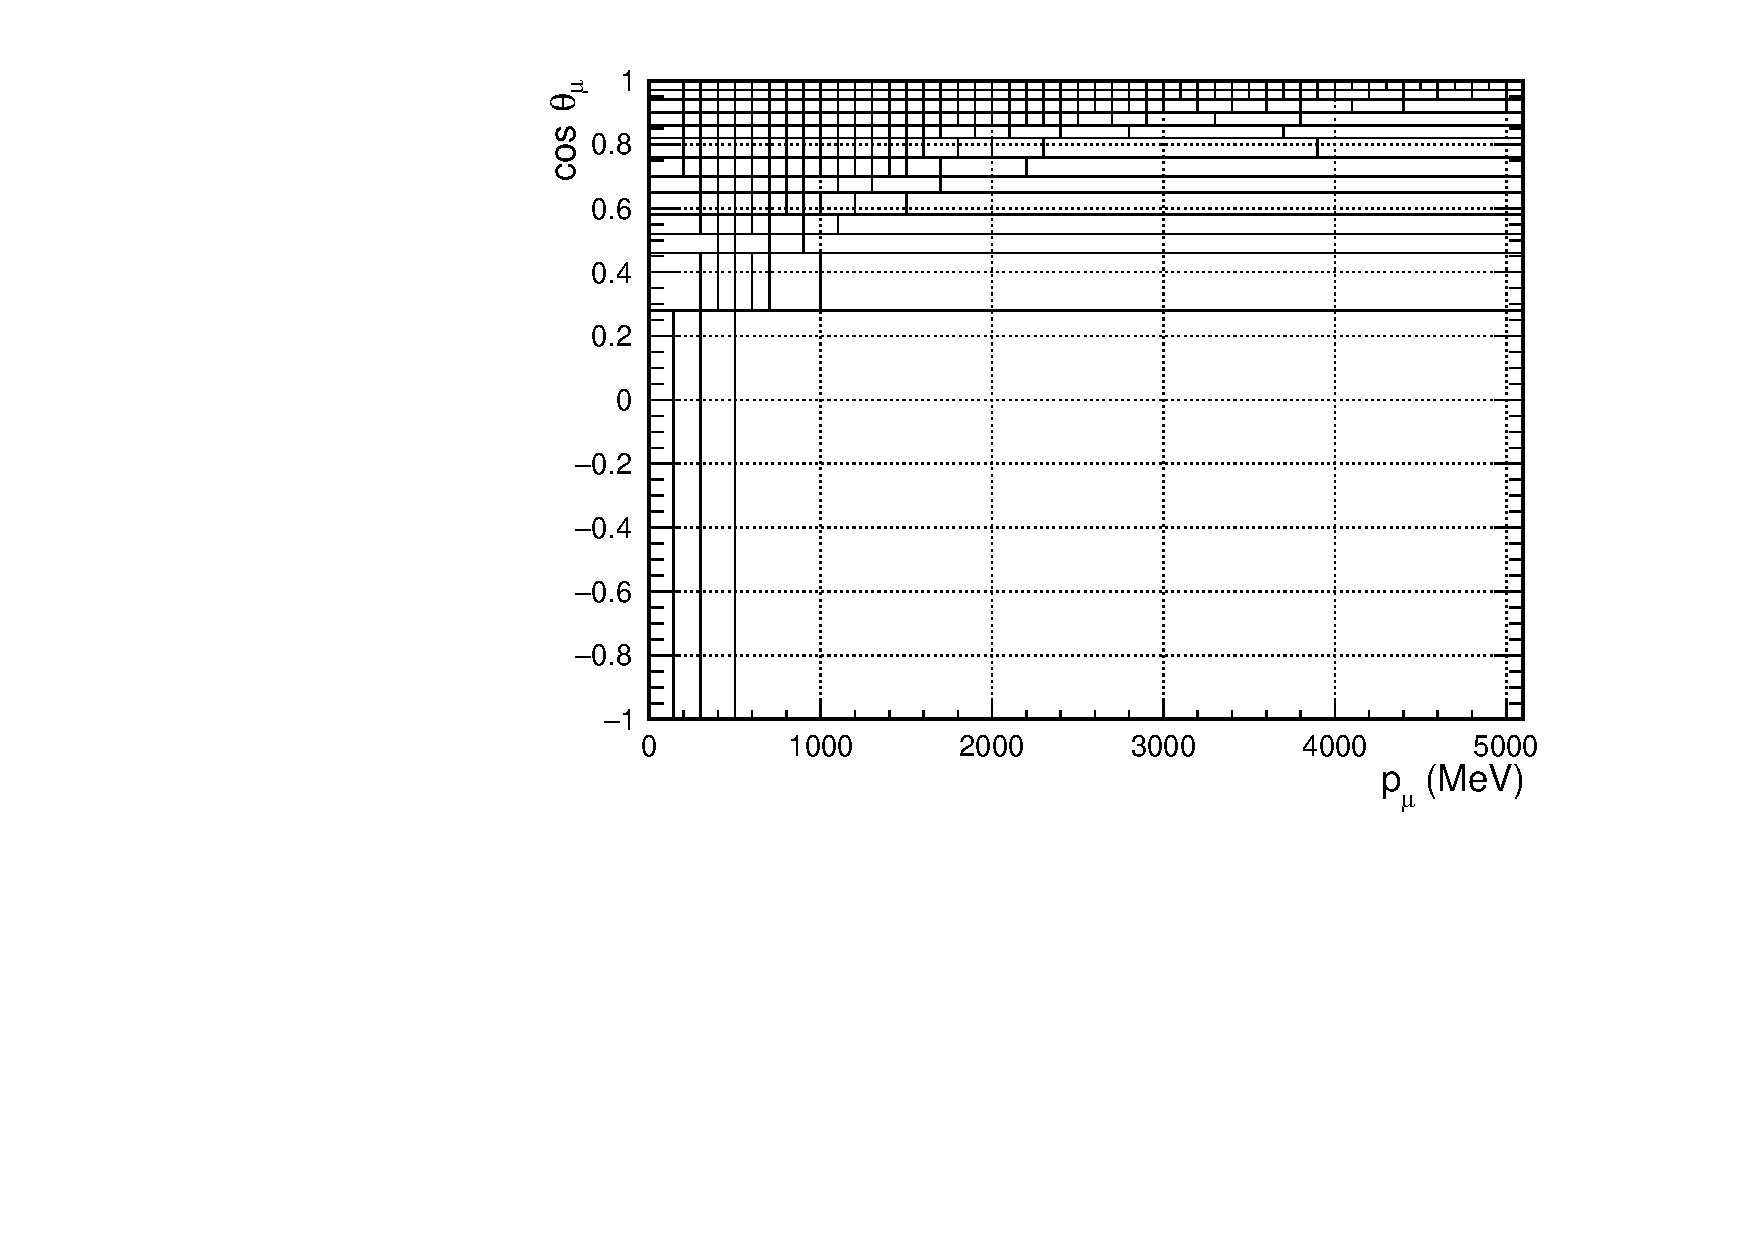
\includegraphics[width=0.95\linewidth]{figs/TH2PolyReset5000_MC_FGD1_numuCC_other}
  \caption{FGD1 FHC $\nu_{\mu}$ Other}
  \label{fig:TH2Poly_Reset5000FGD1_numuCC_other}
\end{subfigure}
\centering
\begin{subfigure}{.32\textwidth}
  \centering
  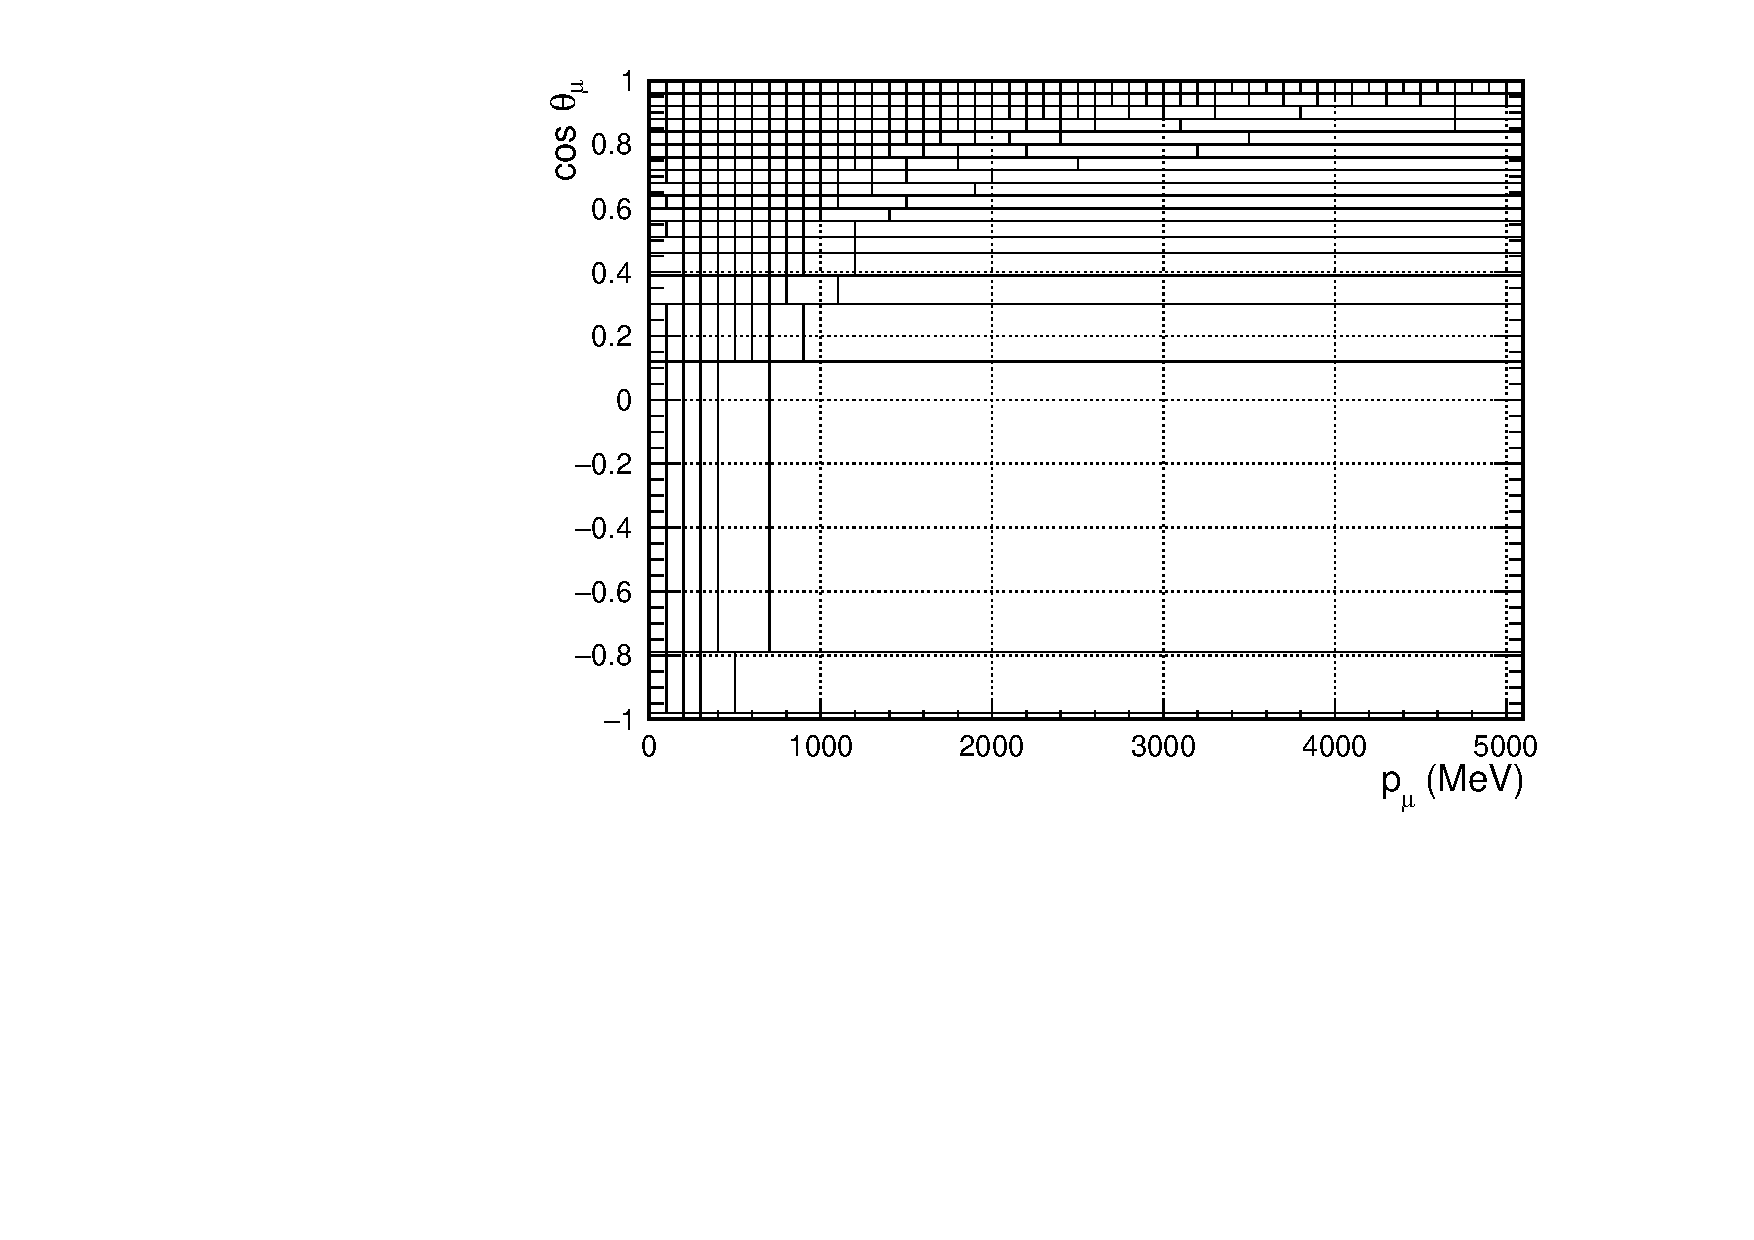
\includegraphics[width=0.95\linewidth]{figs/TH2PolyReset5000_MC_FGD2_numuCC_0pi}
  \caption{FGD2 FHC $\nu_{\mu}$ 0$\pi$}
  \label{fig:TH2Poly_Reset5000FGD2_numuCC_0pi}
\end{subfigure}
\begin{subfigure}{.32\textwidth}
  \centering
  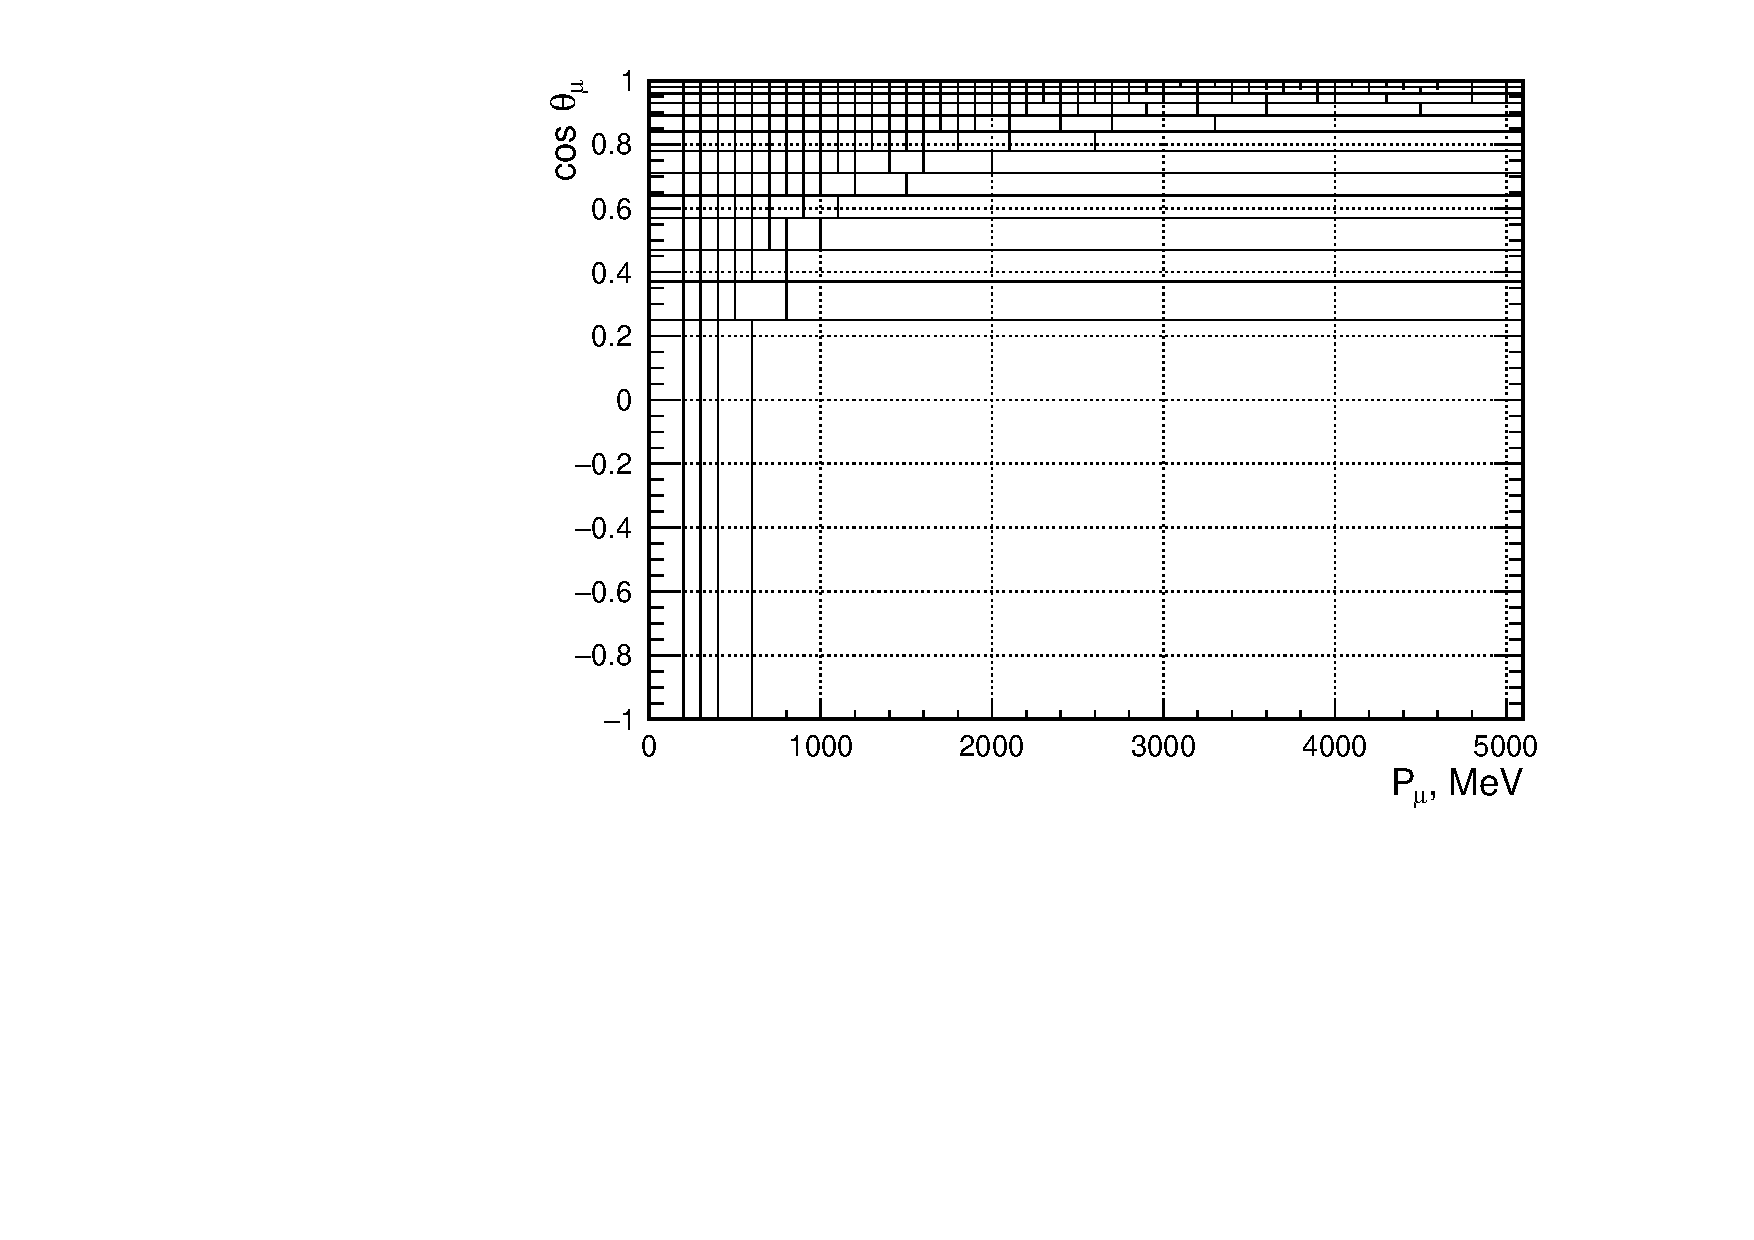
\includegraphics[width=0.95\linewidth]{figs/TH2PolyReset5000_MC_FGD2_numuCC_1pi}
  \caption{FGD2 FHC $\nu_{\mu}$ 1$\pi$}
  \label{fig:TH2Poly_Reset5000FGD2_numuCC_1pi}
\end{subfigure}
\begin{subfigure}{.32\textwidth}
  \centering
  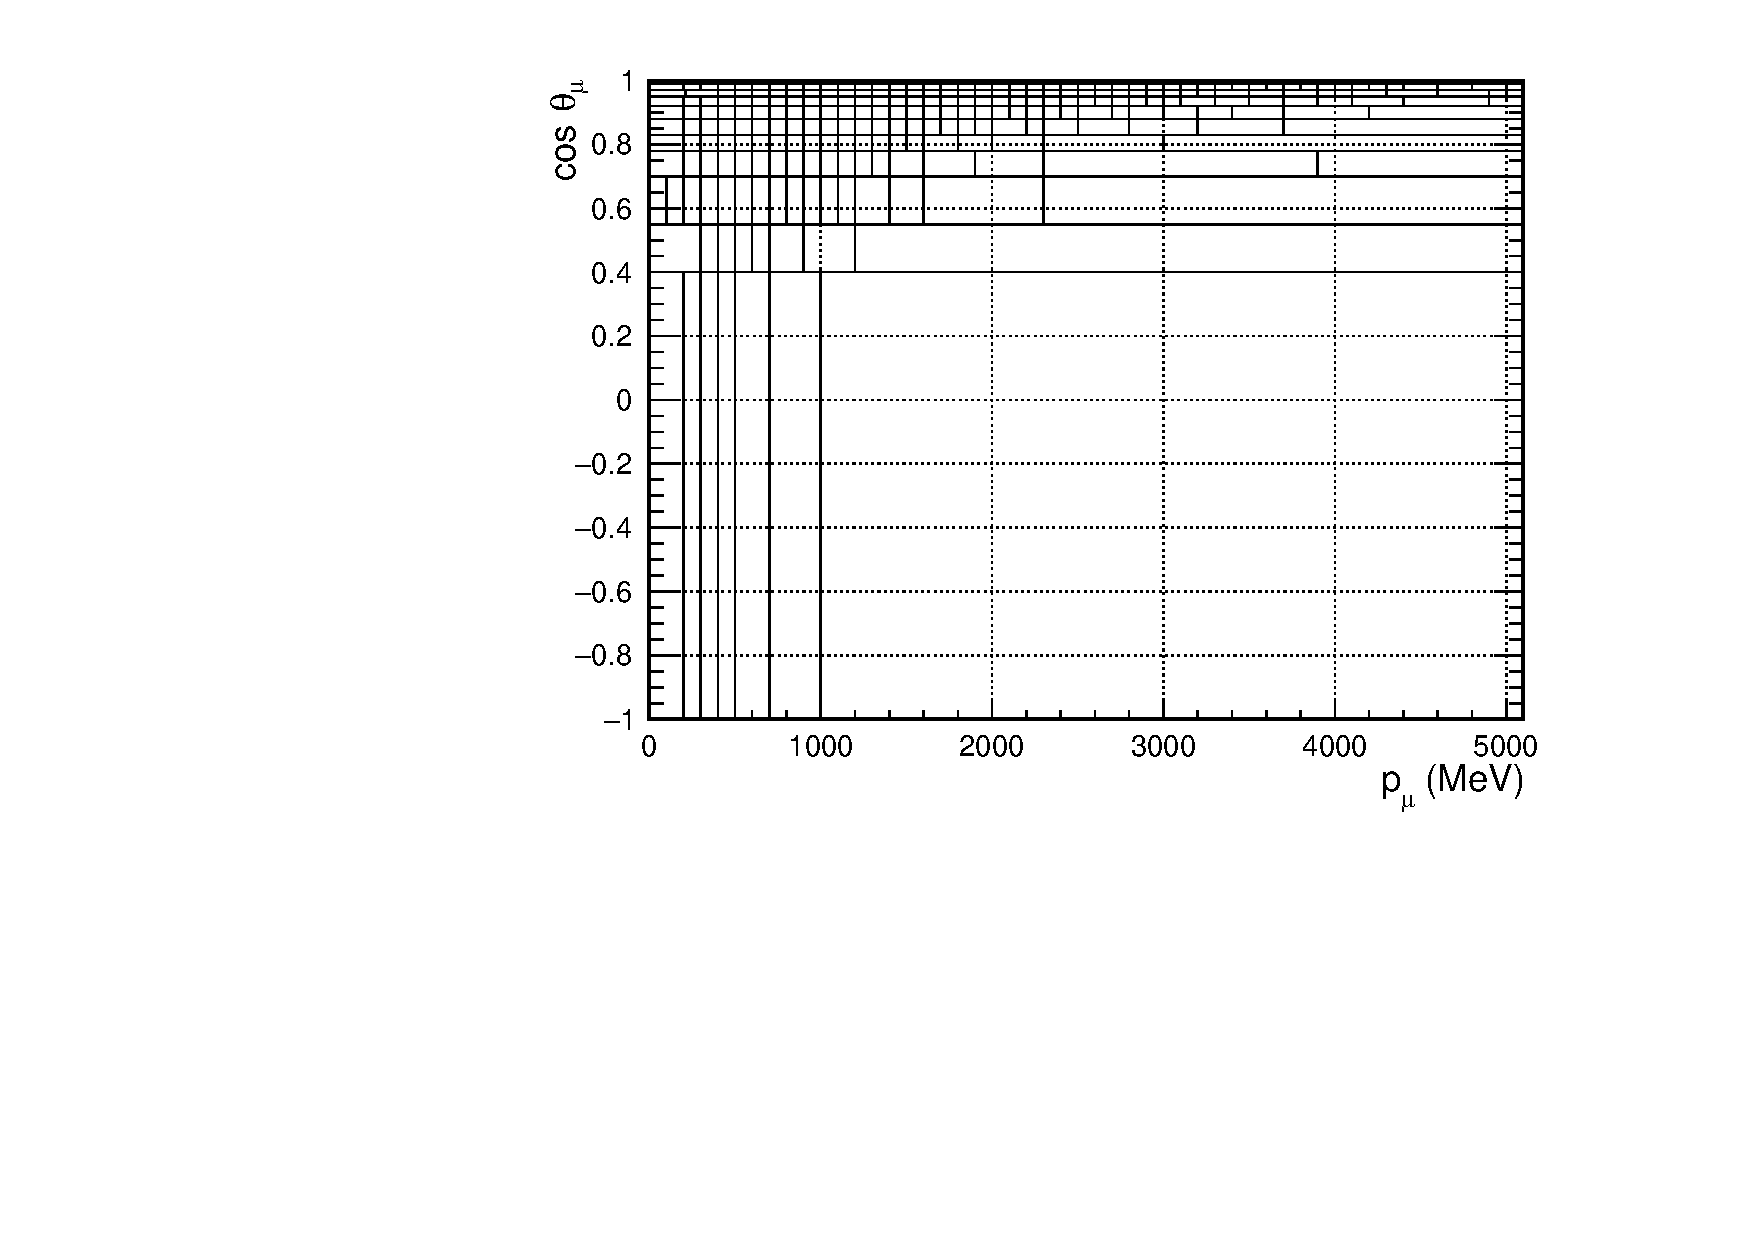
\includegraphics[width=0.95\linewidth]{figs/TH2PolyReset5000_MC_FGD2_numuCC_other}
  \caption{FGD2 FHC $\nu_{\mu}$ Other}
  \label{fig:TH2Poly_Reset5000FGD2_numuCC_other}
\end{subfigure}
\centering
\begin{subfigure}{.32\textwidth}
  \centering
  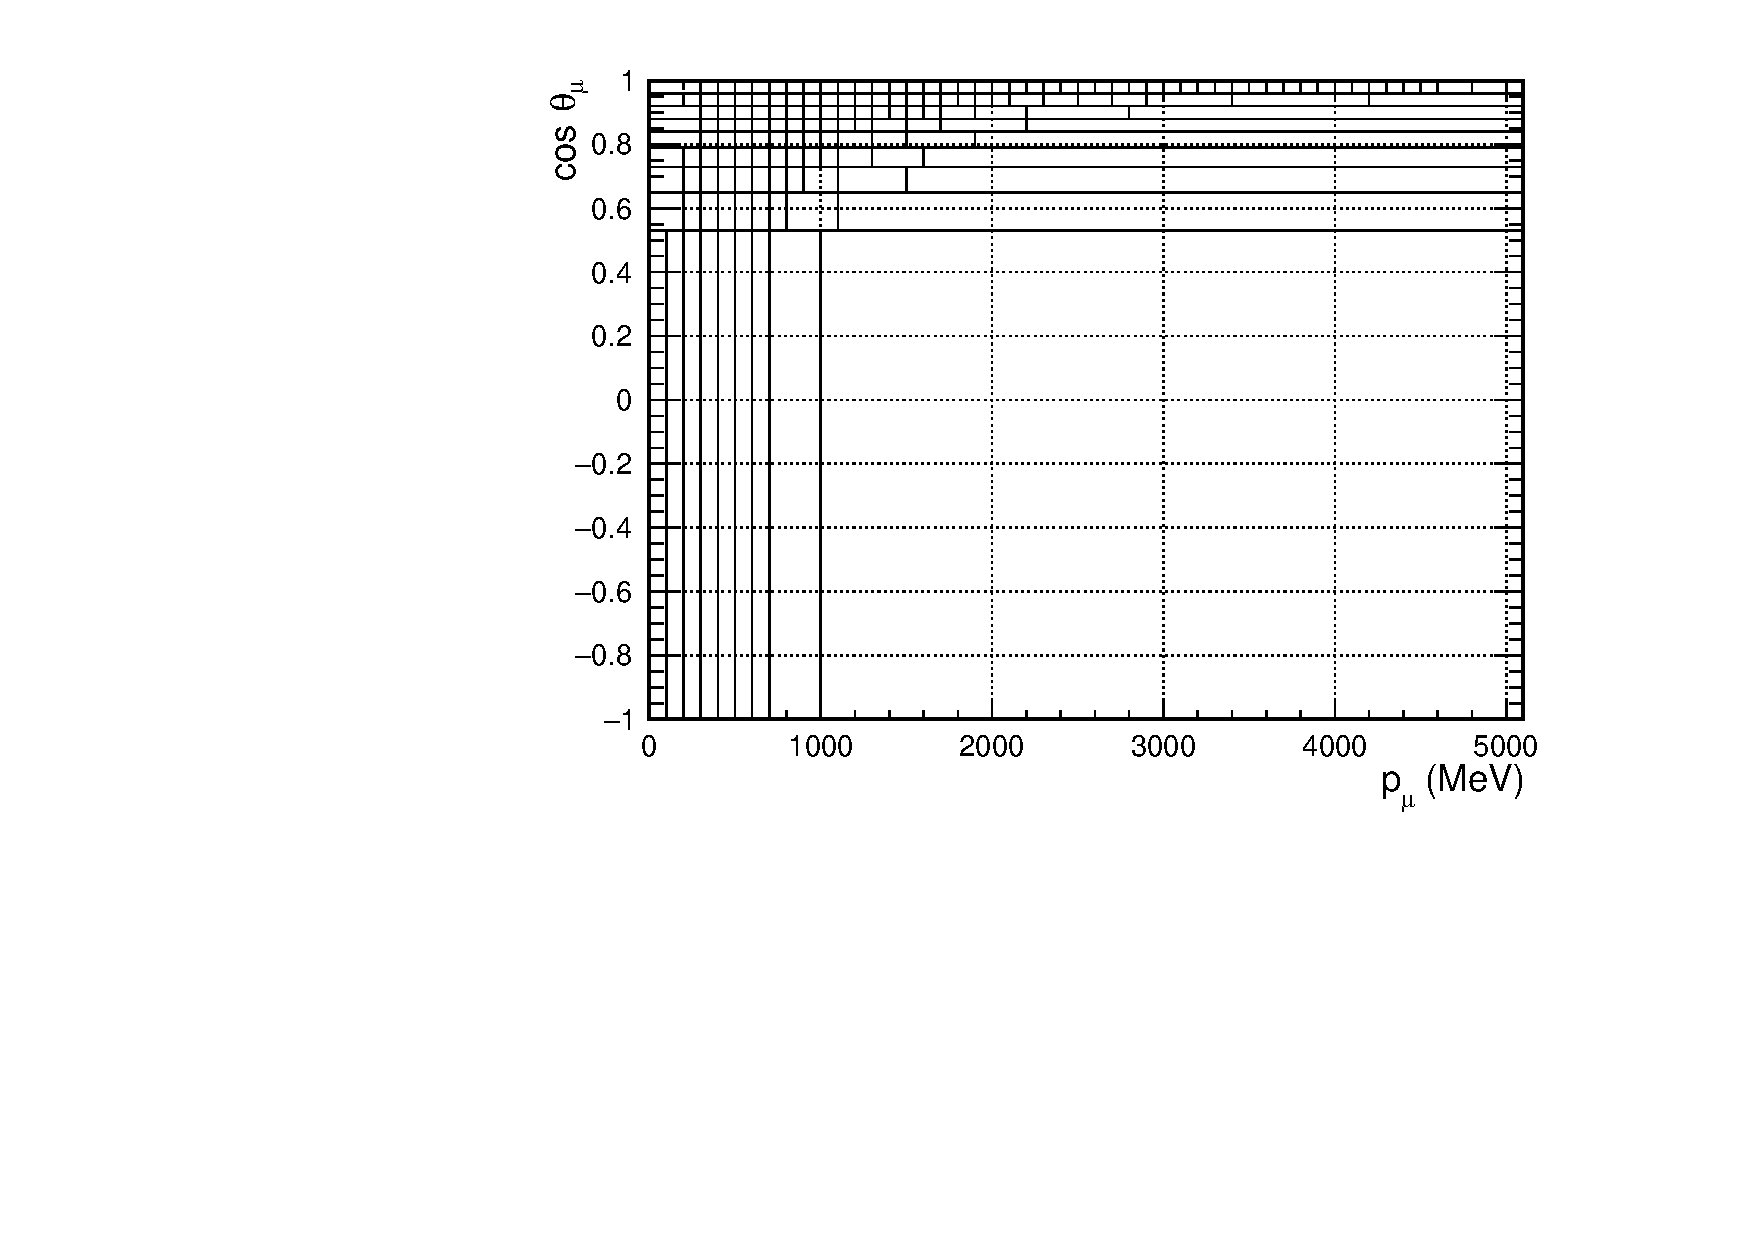
\includegraphics[width=0.95\linewidth]{figs/TH2PolyReset5000_MC_FGD1_anti-numuCC_0pi}
  \caption{FGD1 RHC $\bar{\nu_{\mu}}$ 0$\pi$}
  \label{fig:TH2Poly_Reset5000FGD1_anti-numuCC_0pi}
\end{subfigure}
\begin{subfigure}{.32\textwidth}
  \centering
  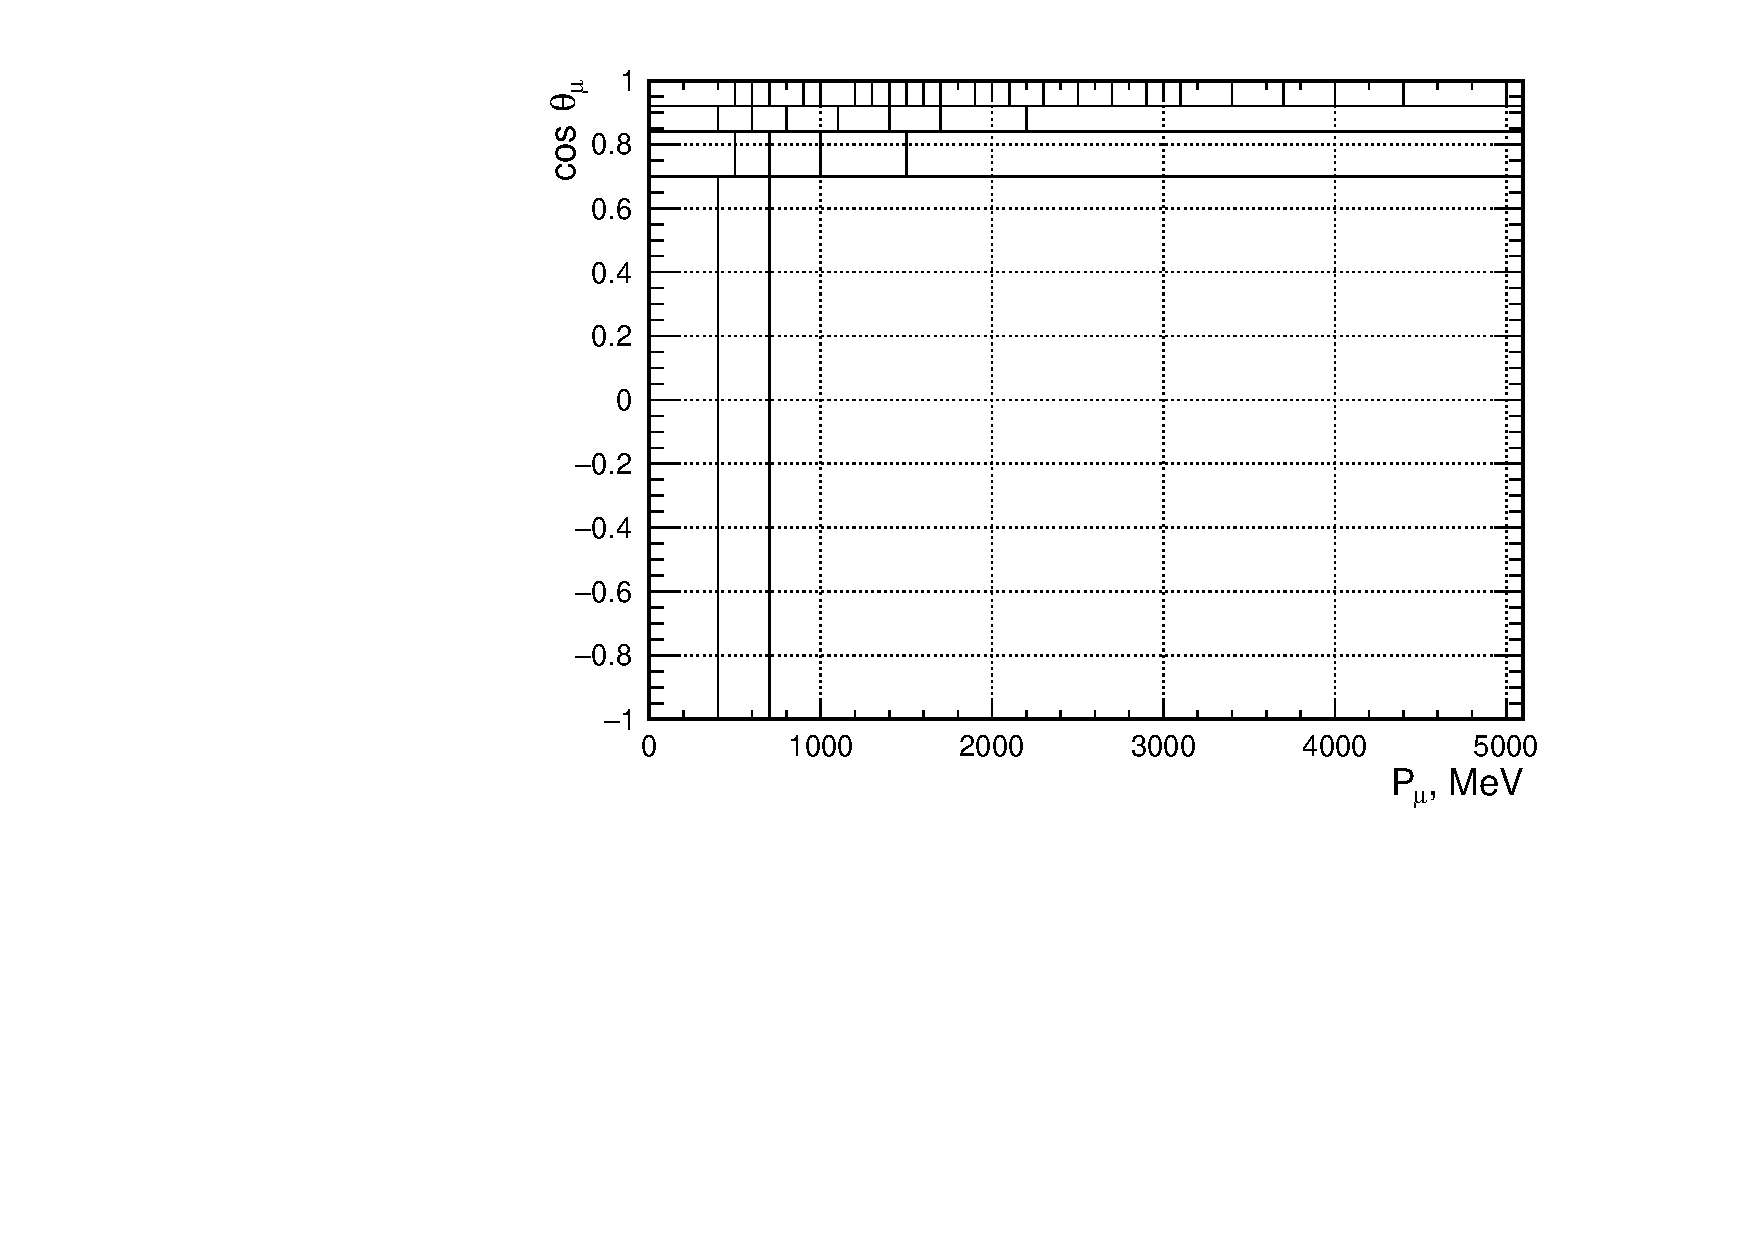
\includegraphics[width=0.95\linewidth]{figs/TH2PolyReset5000_MC_FGD1_anti-numuCC_1pi}
  \caption{FGD1 RHC $\bar{\nu_{\mu}}$ 1$\pi$}
  \label{fig:th2polyTH2Poly_Reset5000FGD1_anti-numuCC_1pi}
\end{subfigure}
\begin{subfigure}{.32\textwidth}
  \centering
  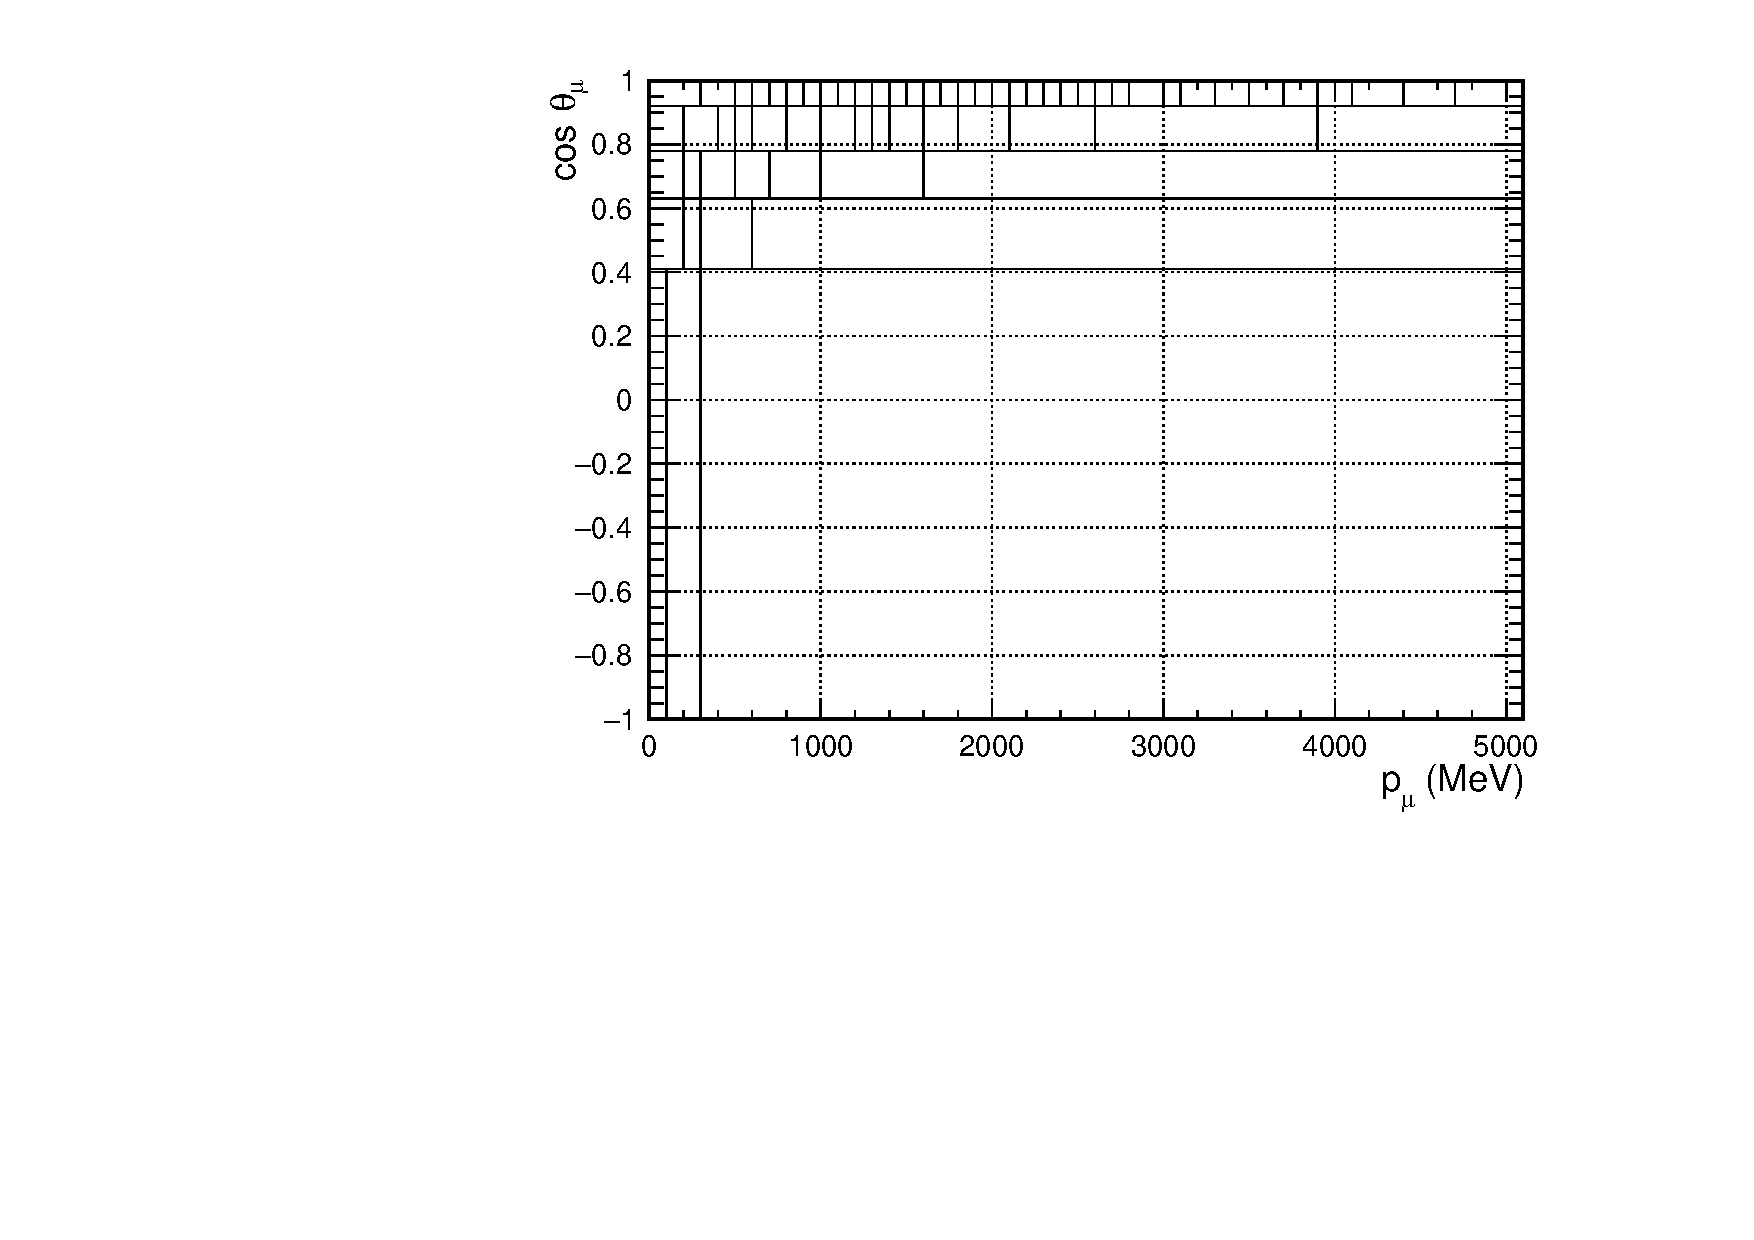
\includegraphics[width=0.95\linewidth]{figs/TH2PolyReset5000_MC_FGD1_anti-numuCC_other}
  \caption{FGD1 RHC $\bar{\nu_{\mu}}$ Other}
  \label{fig:TH2Poly_Reset5000FGD1_anti-numuCC_other}
\end{subfigure}
\centering
\begin{subfigure}{.32\textwidth}
  \centering
  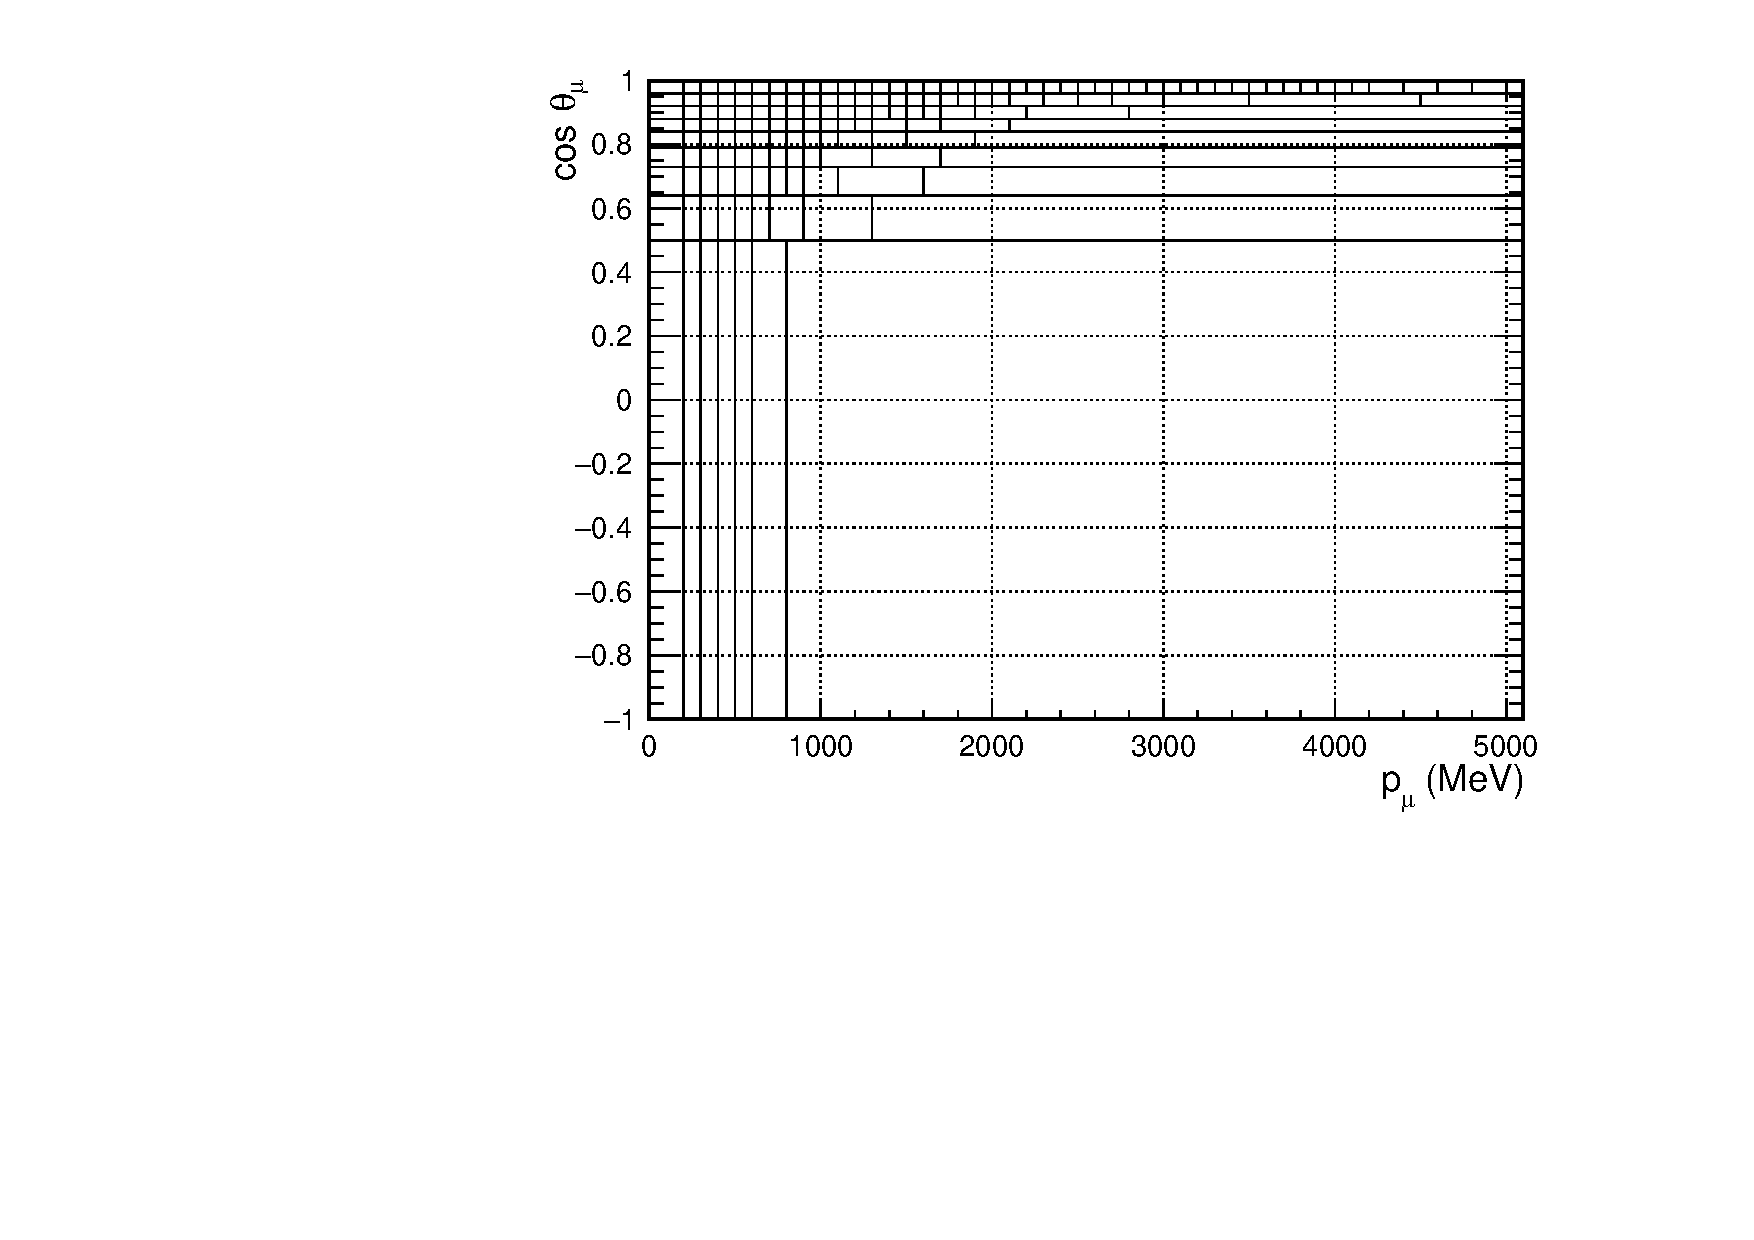
\includegraphics[width=0.95\linewidth]{figs/TH2PolyReset5000_MC_FGD2_anti-numuCC_0pi}
  \caption{FGD2 RHC $\bar{\nu_{\mu}}$ 0$\pi$}
  \label{fig:TH2Poly_Reset5000FGD2_anti-numuCC_0pi}
\end{subfigure}
\begin{subfigure}{.32\textwidth}
  \centering
  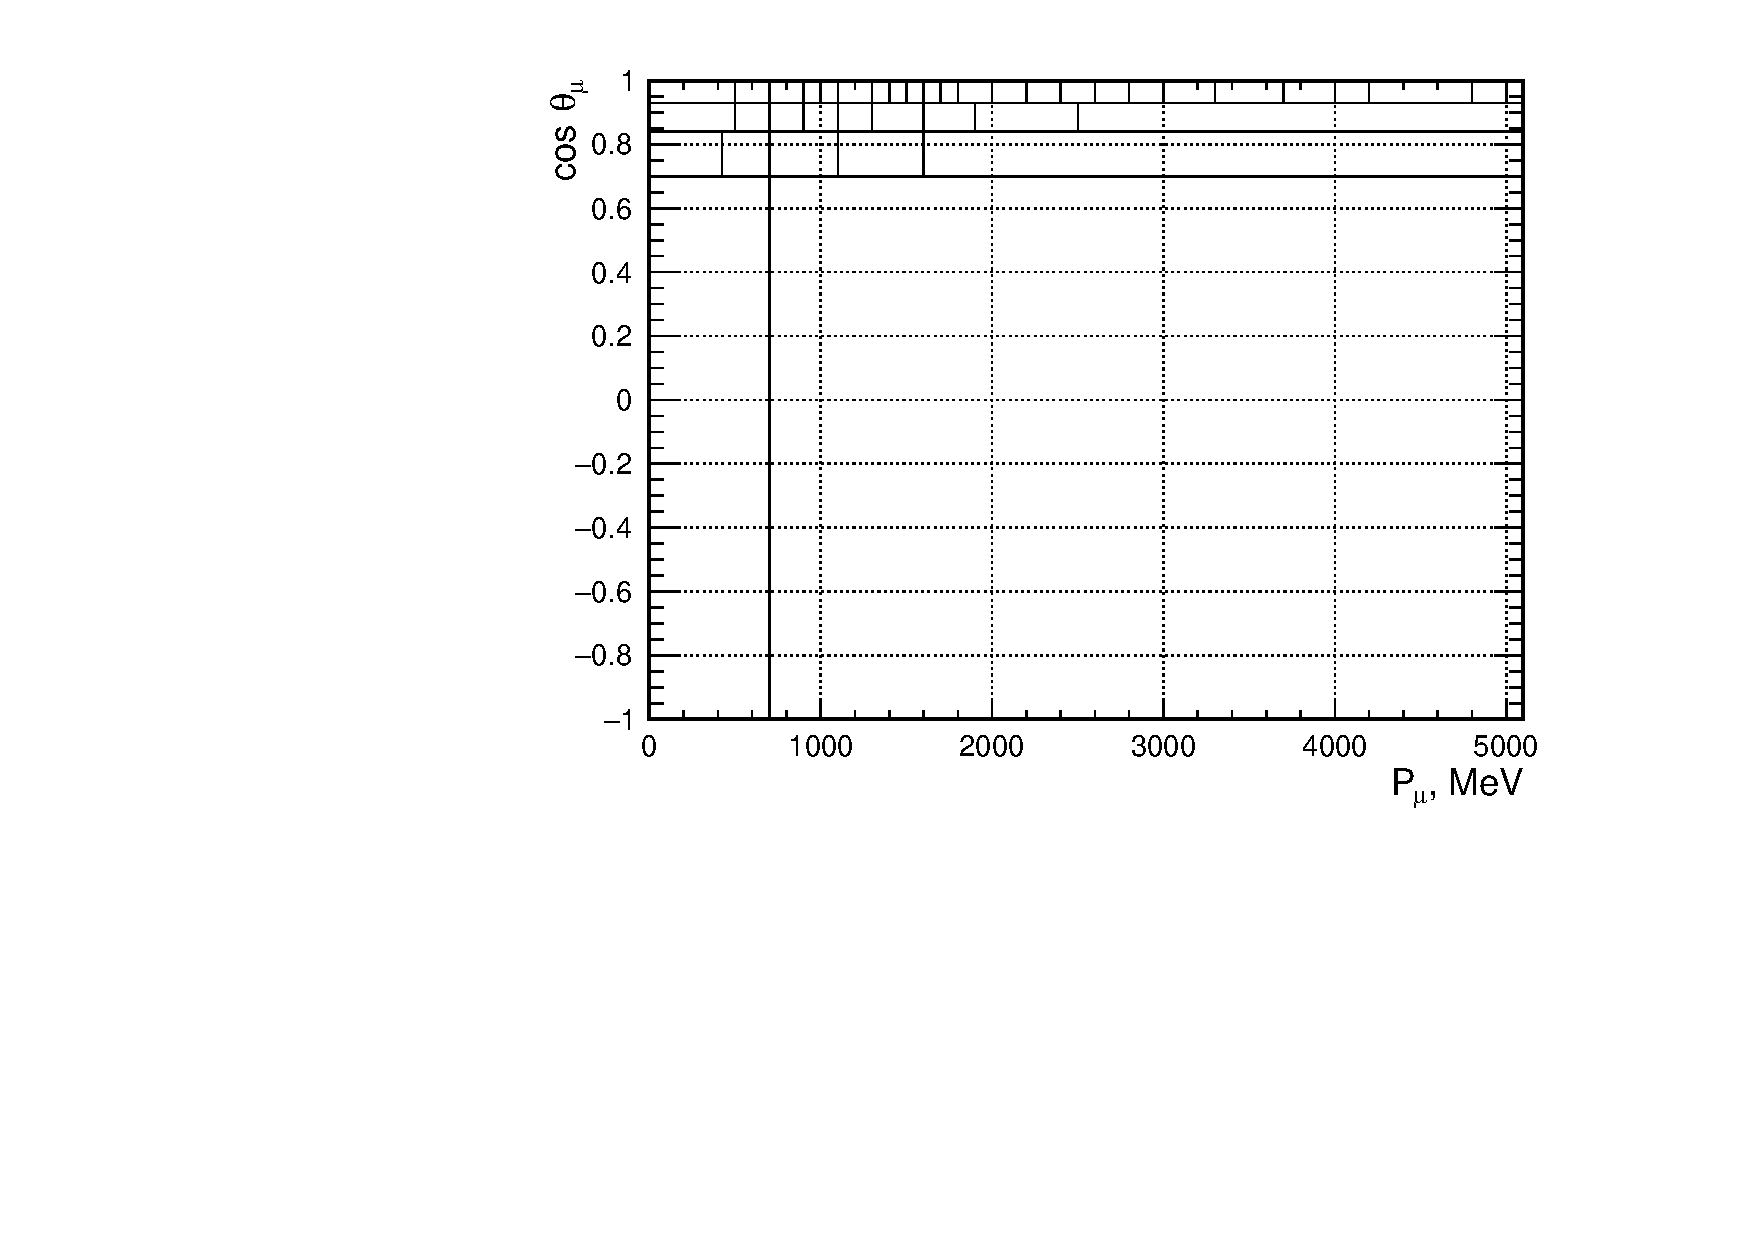
\includegraphics[width=0.95\linewidth]{figs/TH2PolyReset5000_MC_FGD2_anti-numuCC_1pi}
  \caption{FGD2 RHC $\bar{\nu_{\mu}}$ 1$\pi$}
  \label{fig:th2polyTH2Poly_Reset5000FGD2_anti-numuCC_1pi}
\end{subfigure}
\begin{subfigure}{.32\textwidth}
  \centering
  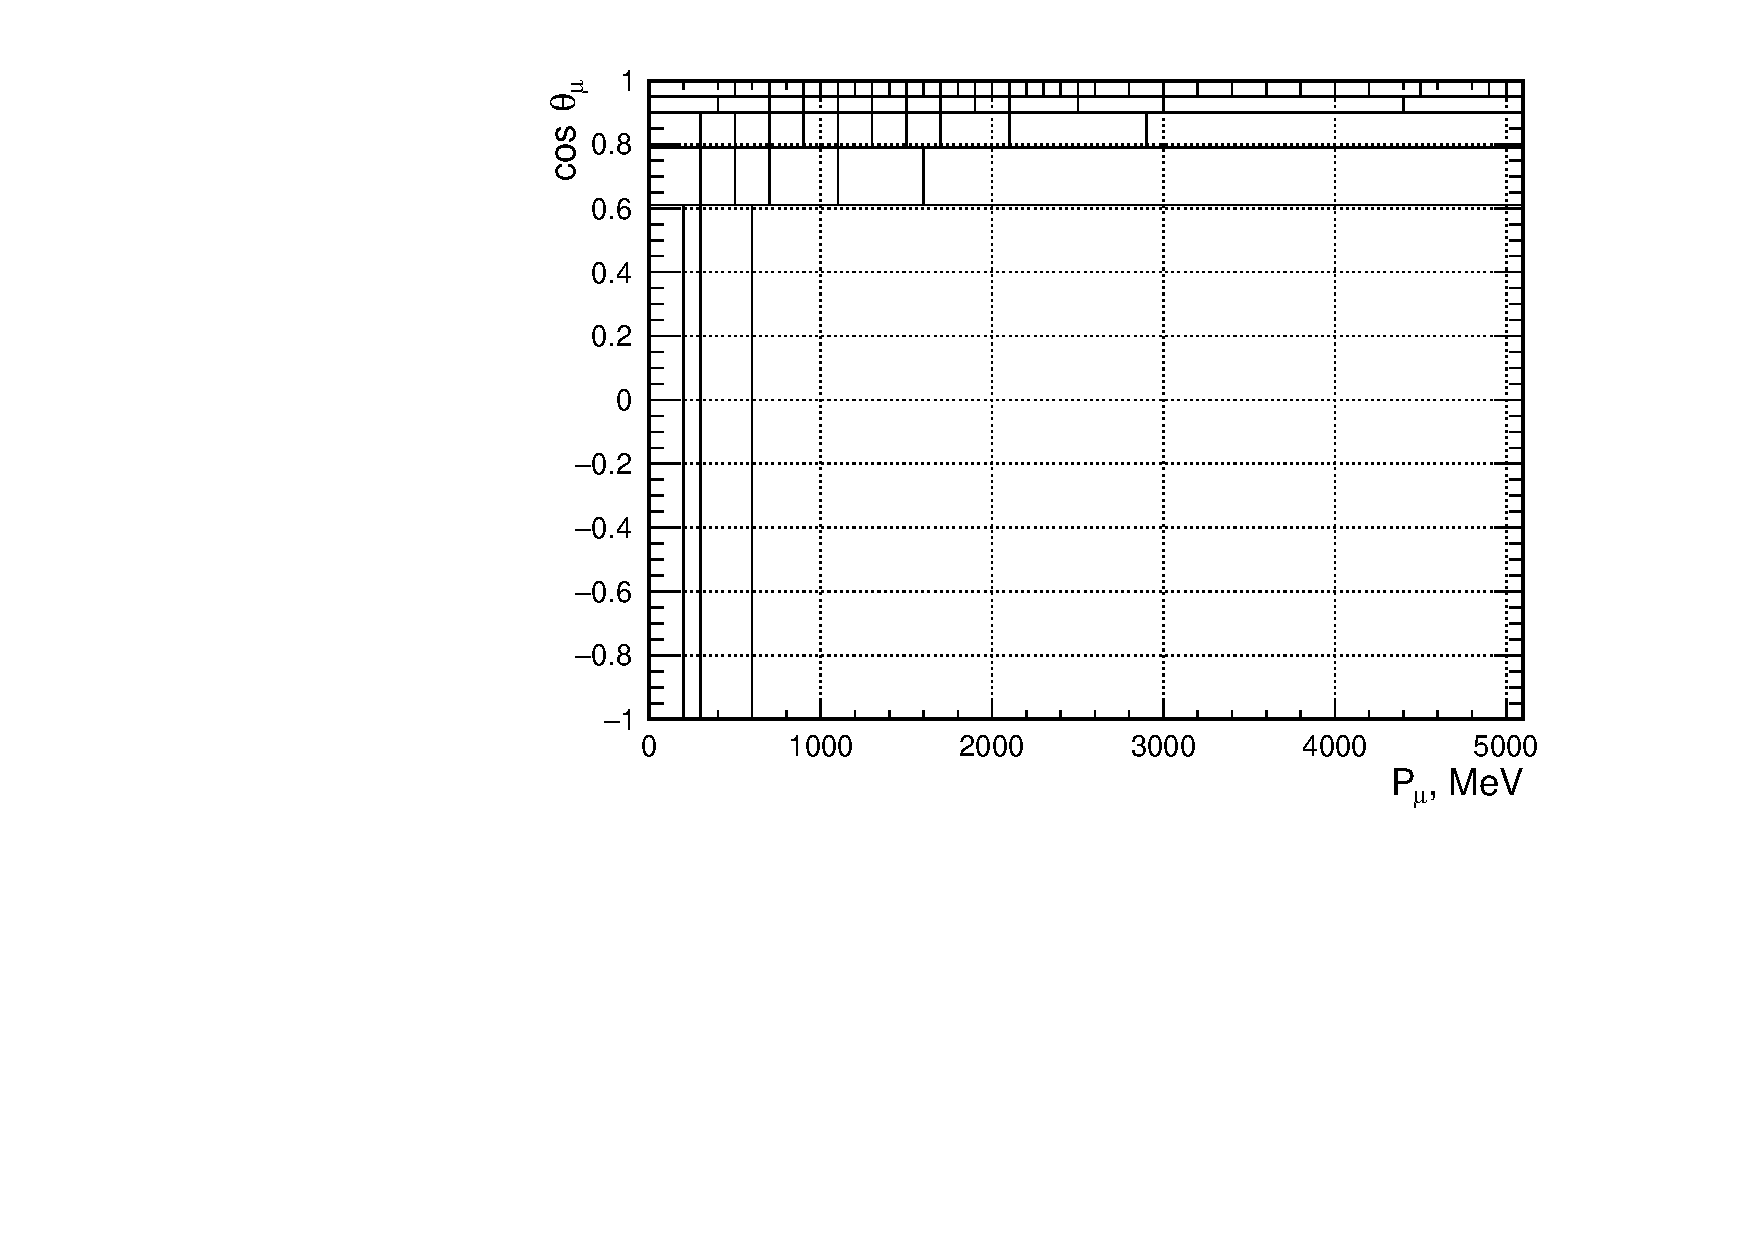
\includegraphics[width=0.95\linewidth]{figs/TH2PolyReset5000_MC_FGD2_anti-numuCC_other}
  \caption{FGD2 RHC $\bar{\nu_{\mu}}$ Other}
  \label{fig:TH2Poly_Reset5000FGD2_anti-numuCC_other}
\end{subfigure}
\begin{subfigure}{.32\textwidth}
  \centering
  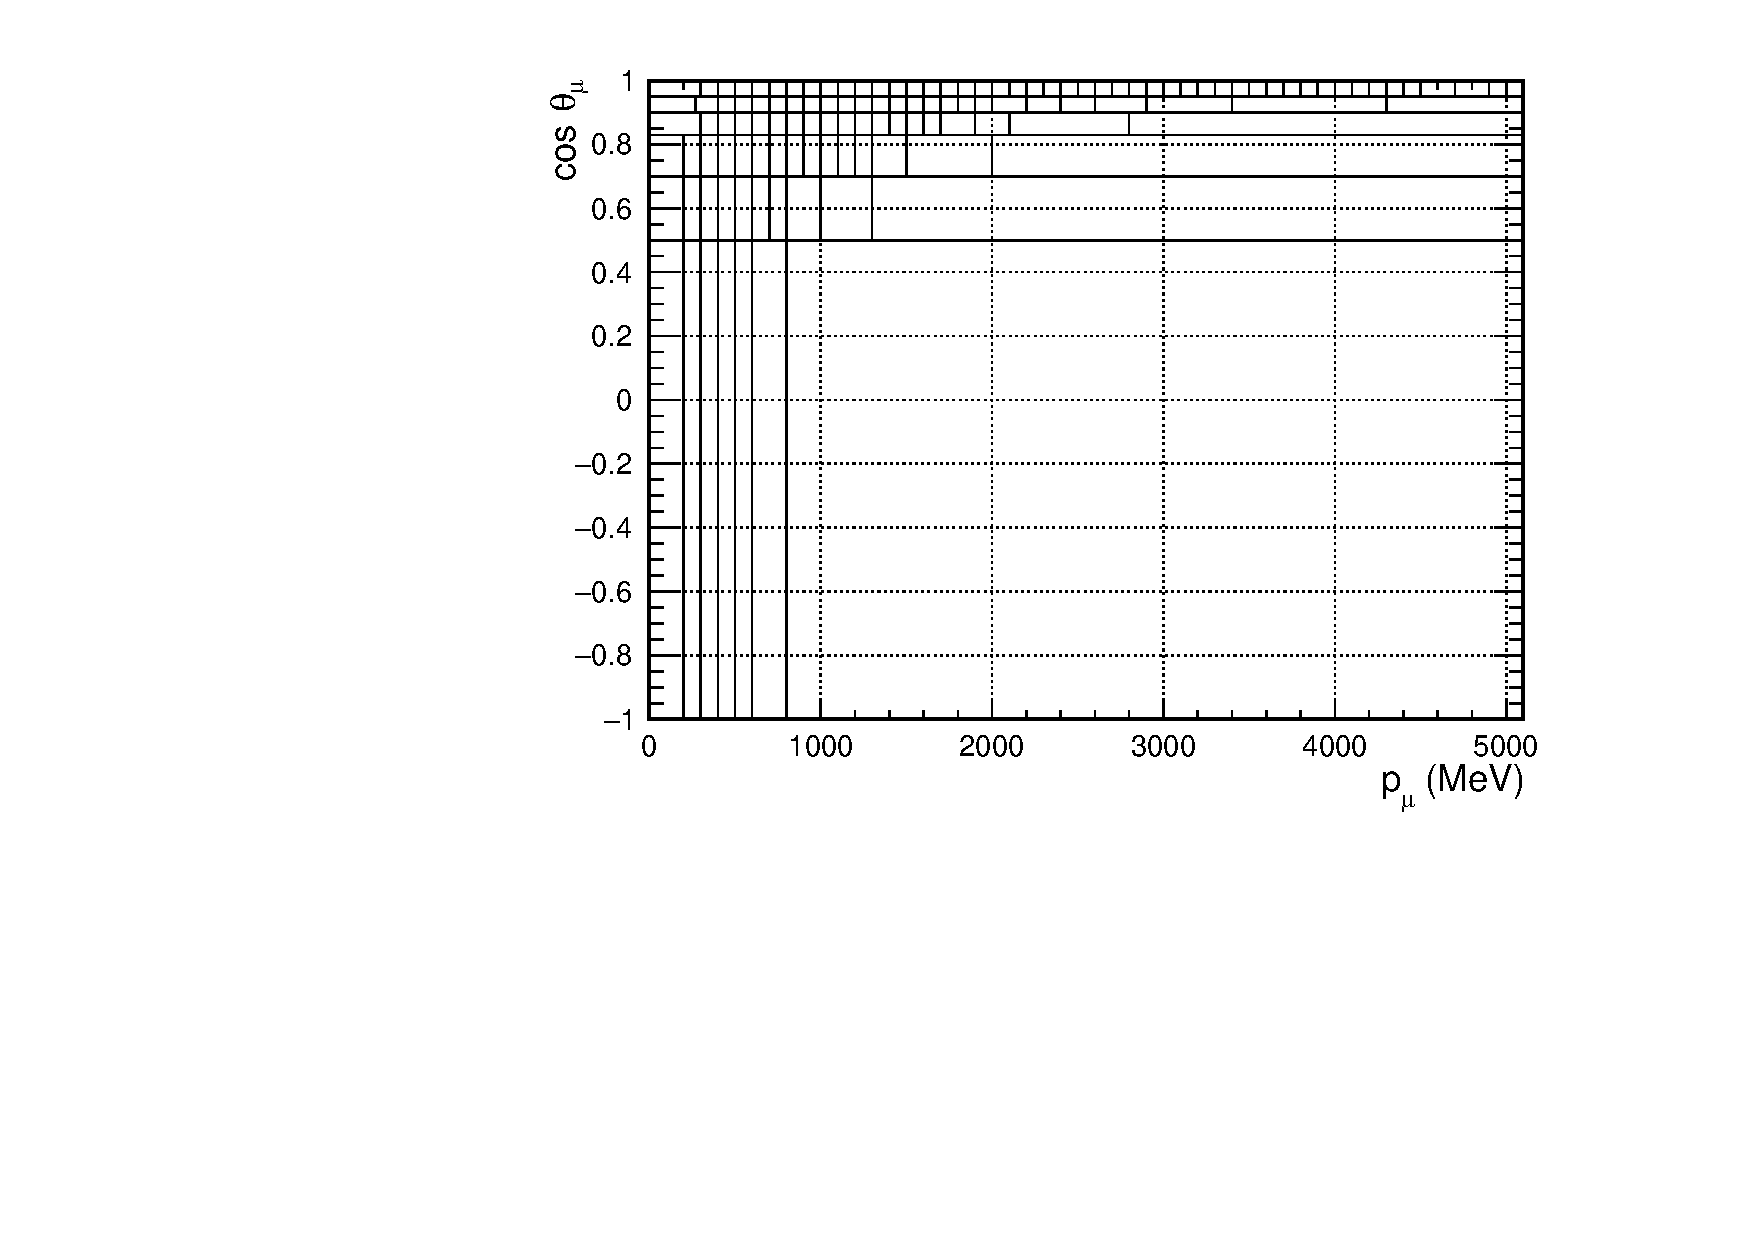
\includegraphics[width=0.95\linewidth]{figs/TH2PolyReset5000_MC_FGD1_NuMuBkg_CC0pi_in_AntiNu_Mode}
  \caption{FGD1 RHC $\nu_{\mu}$ 0$\pi$}
  \label{fig:TH2Poly_Reset5000FGD1_NuMuBkg_CC0pi_in_AntiNu_Mode}
\end{subfigure}
\begin{subfigure}{.32\textwidth}
  \centering
  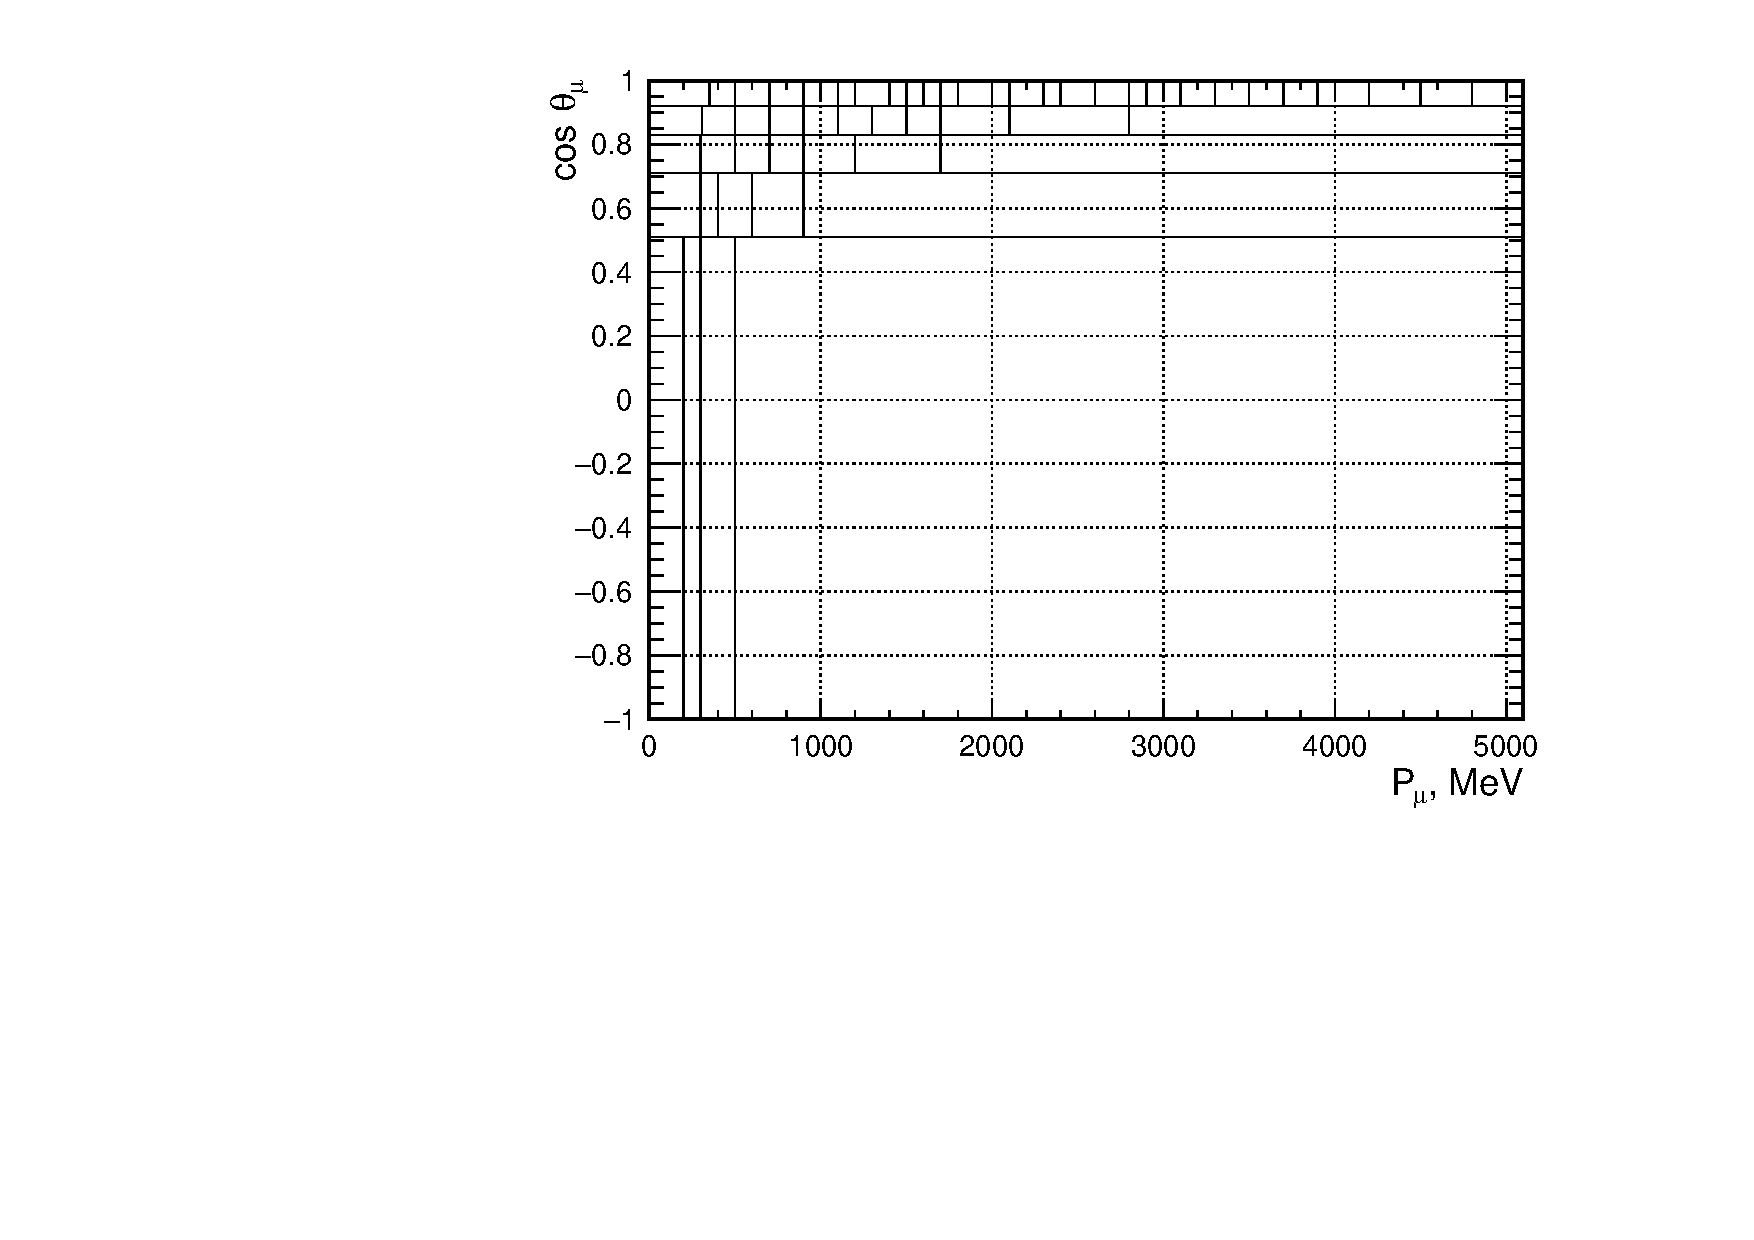
\includegraphics[width=0.95\linewidth]{figs/TH2PolyReset5000_MC_FGD1_NuMuBkg_CC1pi_in_AntiNu_Mode}
  \caption{FGD1 RHC $\nu_{\mu}$ 1$\pi$}
  \label{fig:TH2Poly_Reset5000FGD1_NuMuBkg_CC1pi_in_AntiNu_Mode}
\end{subfigure}
\begin{subfigure}{.32\textwidth}
  \centering
  \includegraphics[width=0.95\linewidth]{figs/TH2PolyReset5000_MC_FGD1_NuMuBkg_CCOther_in_AntiNu_Mode}
  \caption{FGD1 RHC $\nu_{\mu}$ Other}
  \label{fig:TH2Poly_Reset5000FGD1_NuMuBkg_CCOther_in_AntiNu_Mode}
\end{subfigure}
\begin{subfigure}{.32\textwidth}
  \centering
  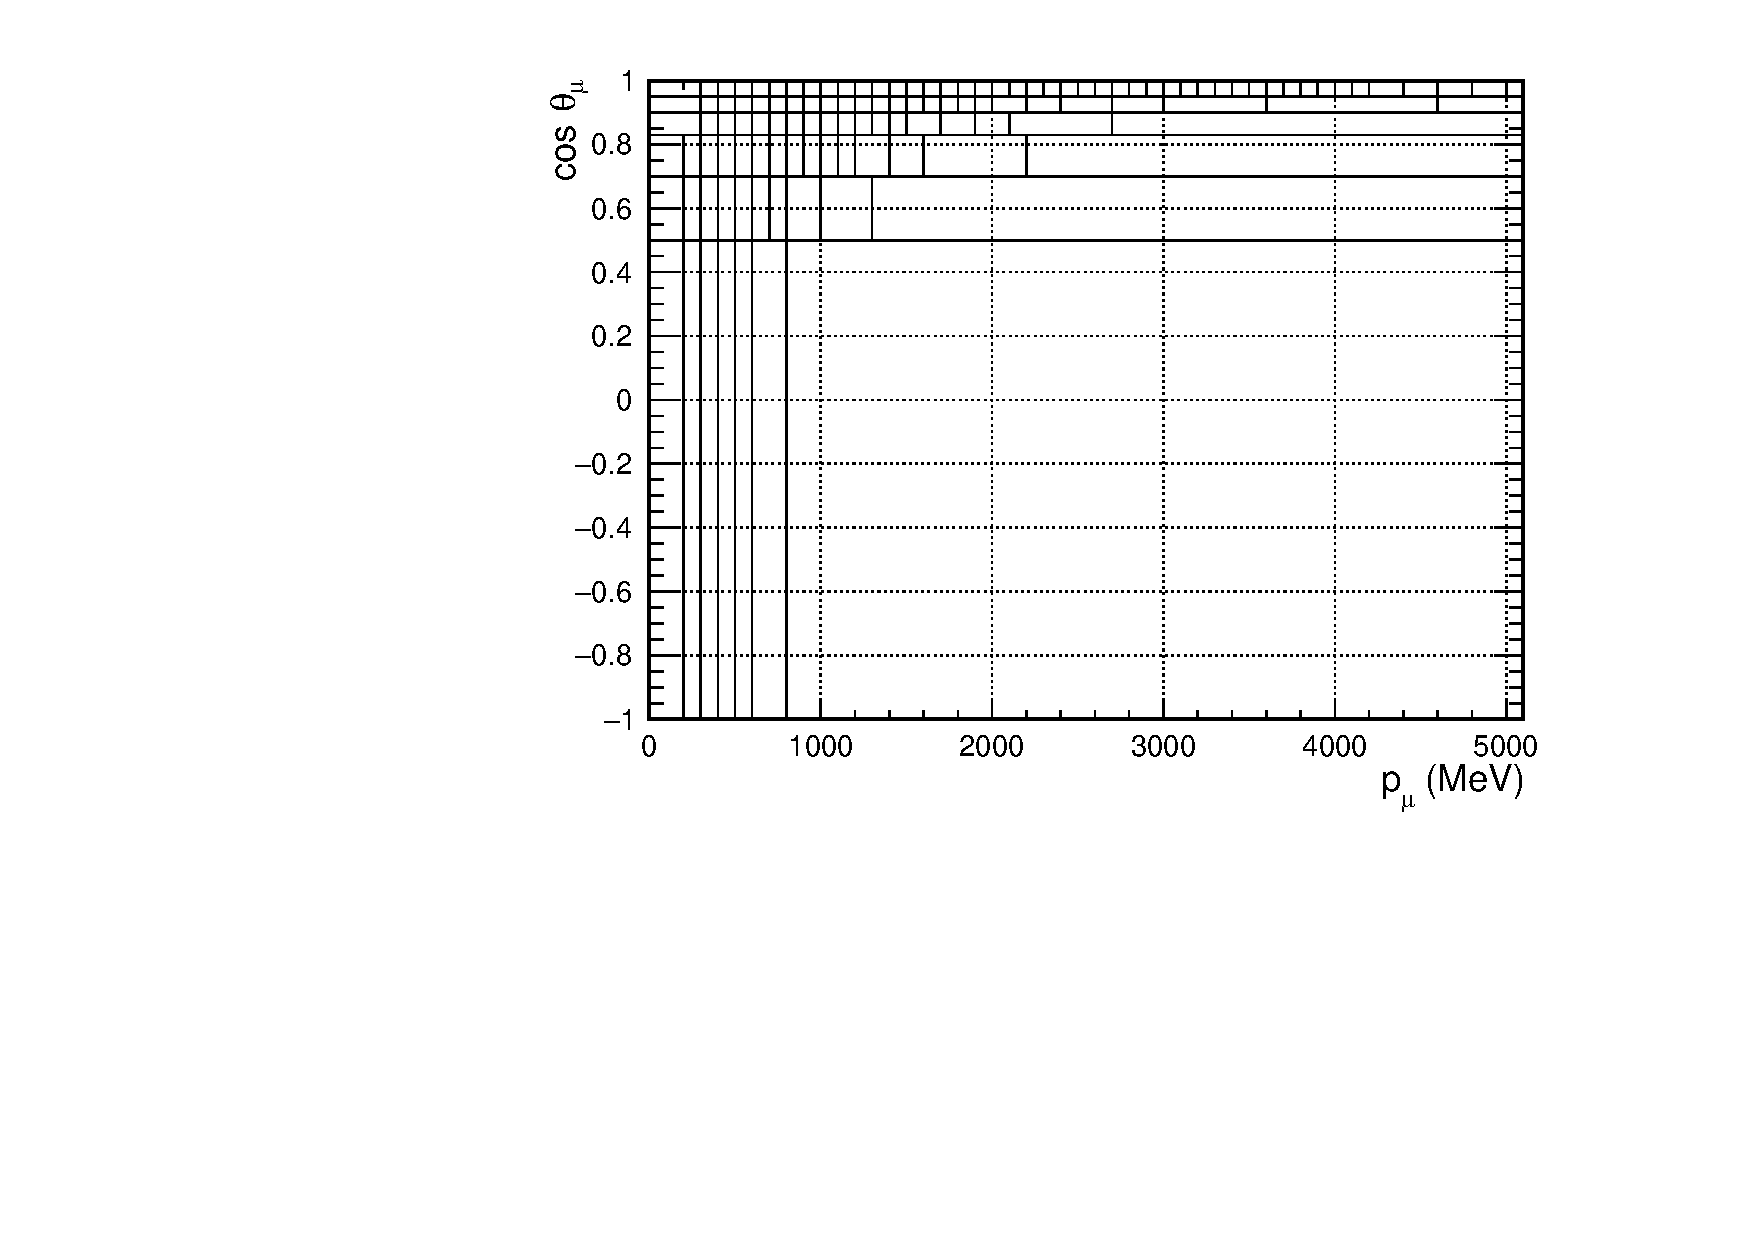
\includegraphics[width=0.95\linewidth]{figs/TH2PolyReset5000_MC_FGD2_NuMuBkg_CC0pi_in_AntiNu_Mode}
  \caption{FGD2 RHC $\nu_{\mu}$ 0$\pi$}
  \label{fig:TH2Poly_Reset5000FGD2_NuMuBkg_CC0pi_in_AntiNu_Mode}
\end{subfigure}
\begin{subfigure}{.32\textwidth}
  \centering
  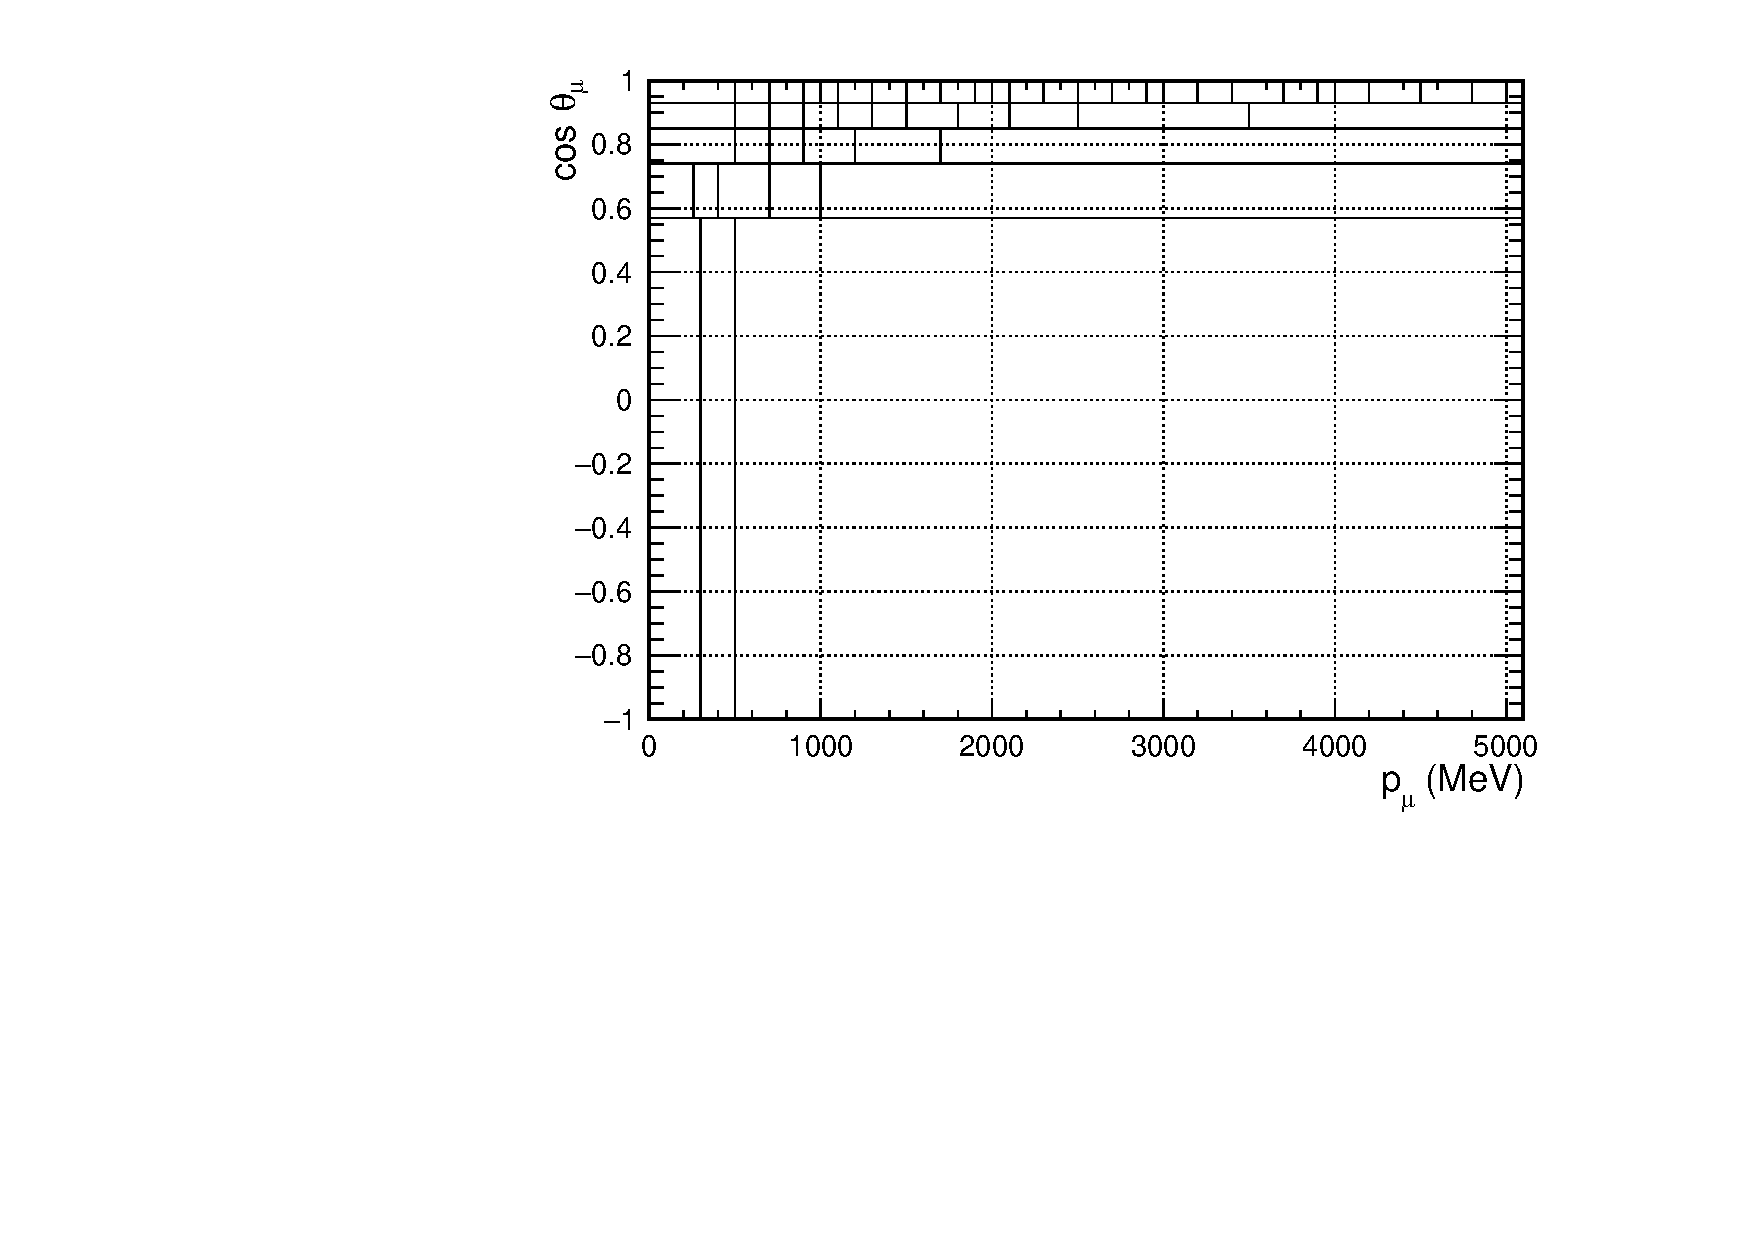
\includegraphics[width=0.95\linewidth]{figs/TH2PolyReset5000_MC_FGD2_NuMuBkg_CC1pi_in_AntiNu_Mode}
  \caption{FGD2 RHC $\nu_{\mu}$ 1$\pi$}
  \label{fig:TH2Poly_Reset5000FGD2_NuMuBkg_CC1pi_in_AntiNu_Mode}
\end{subfigure}
\begin{subfigure}{.32\textwidth}
  \centering
  \includegraphics[width=0.95\linewidth]{figs/TH2PolyReset5000_MC_FGD2_NuMuBkg_CCOther_in_AntiNu_Mode}
  \caption{FGD2 RHC $\nu_{\mu}$ Other}
  \label{fig:TH2Poly_Reset5000FGD2_NuMuBkg_CCOther_in_AntiNu_Mode}
\end{subfigure}
\caption{Non-uniform rectangular binning used in this analysis for each sample. The x-axis is reduced to better show the smaller bins at low momentum and high angle.}
\label{fig:th2polybinreset5000}
\end{figure}

\begin{figure}
\centering
\begin{subfigure}{.32\textwidth}
  \centering
  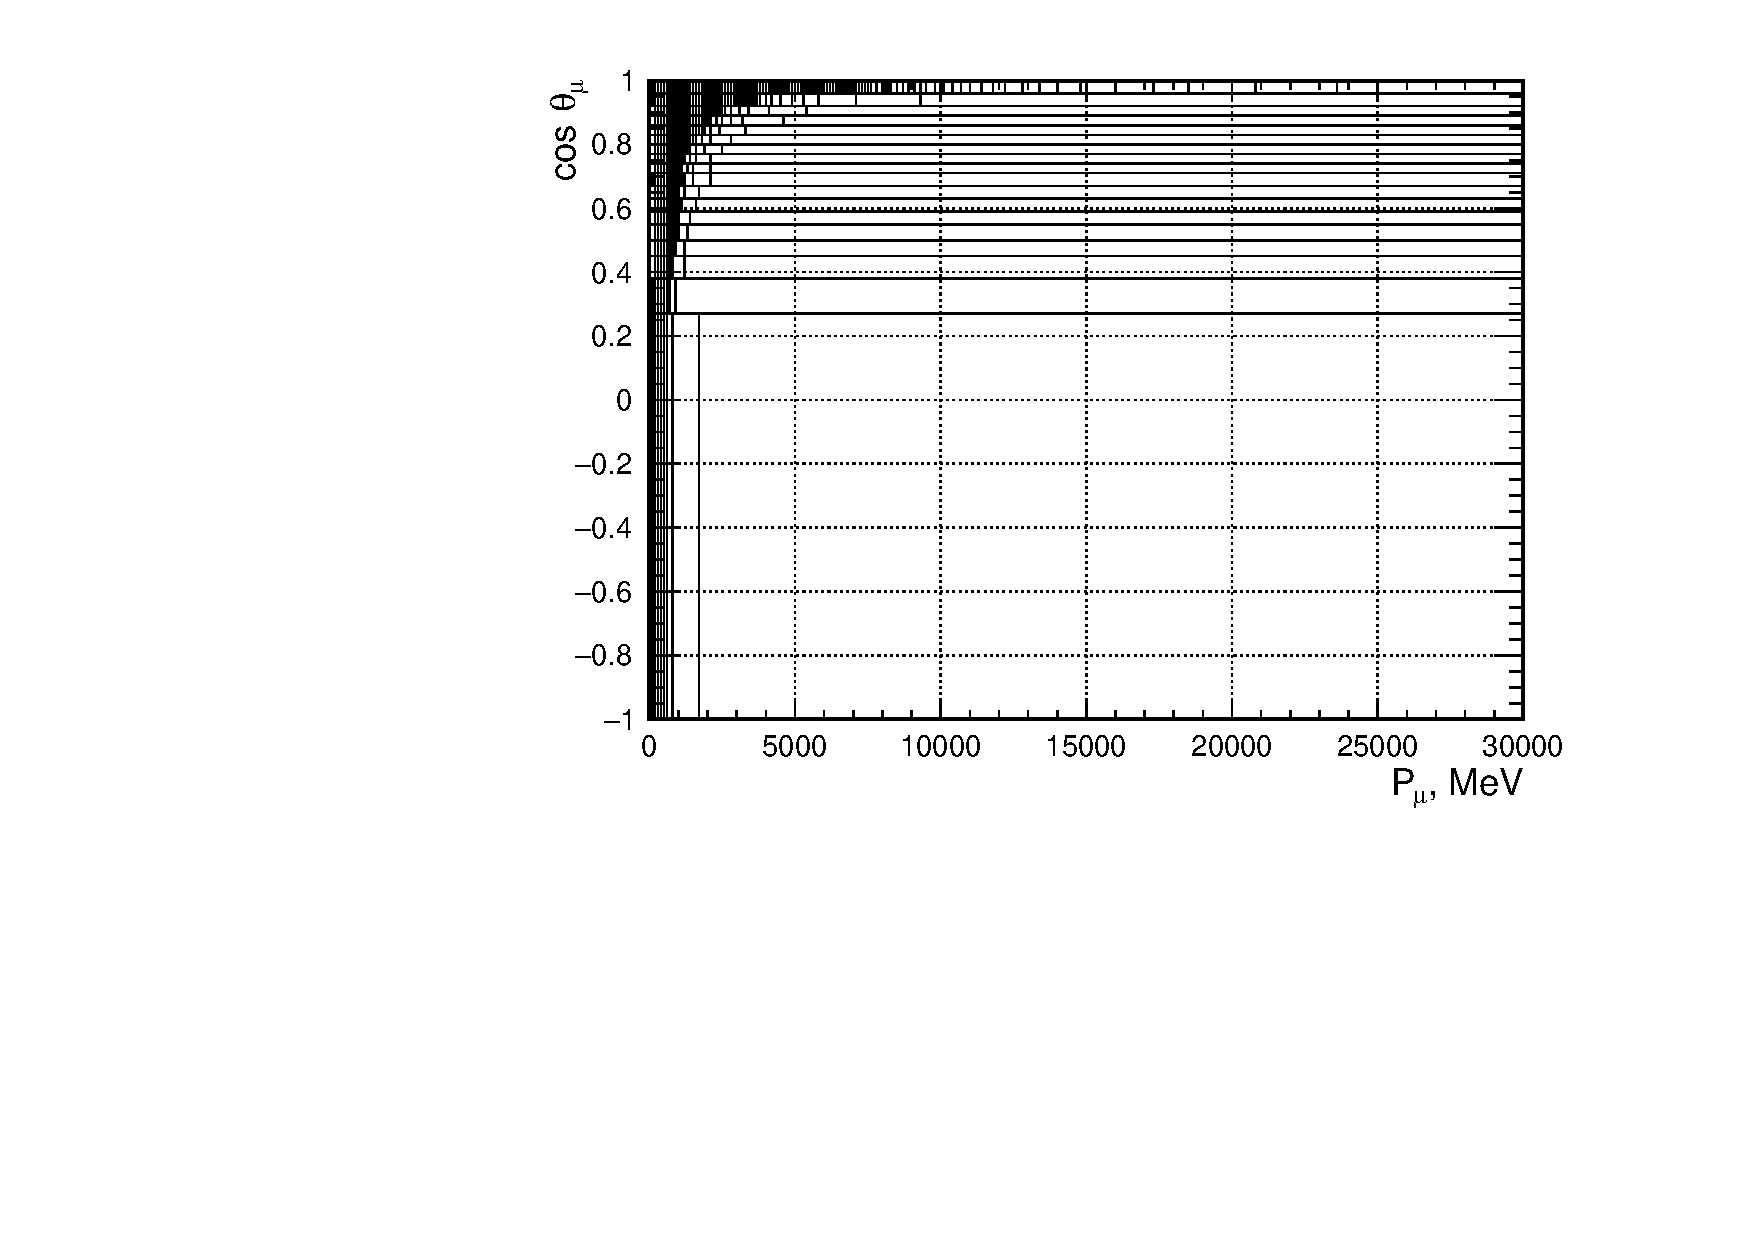
\includegraphics[width=0.95\linewidth]{figs/TH2PolyReset_MC_FGD1_numuCC_0pi}
  \caption{FGD1 FHC $\nu_{\mu}$ 0$\pi$}
  \label{fig:TH2Poly_ResetFGD1_numuCC_0pi}
\end{subfigure}
\begin{subfigure}{.32\textwidth}
  \centering
  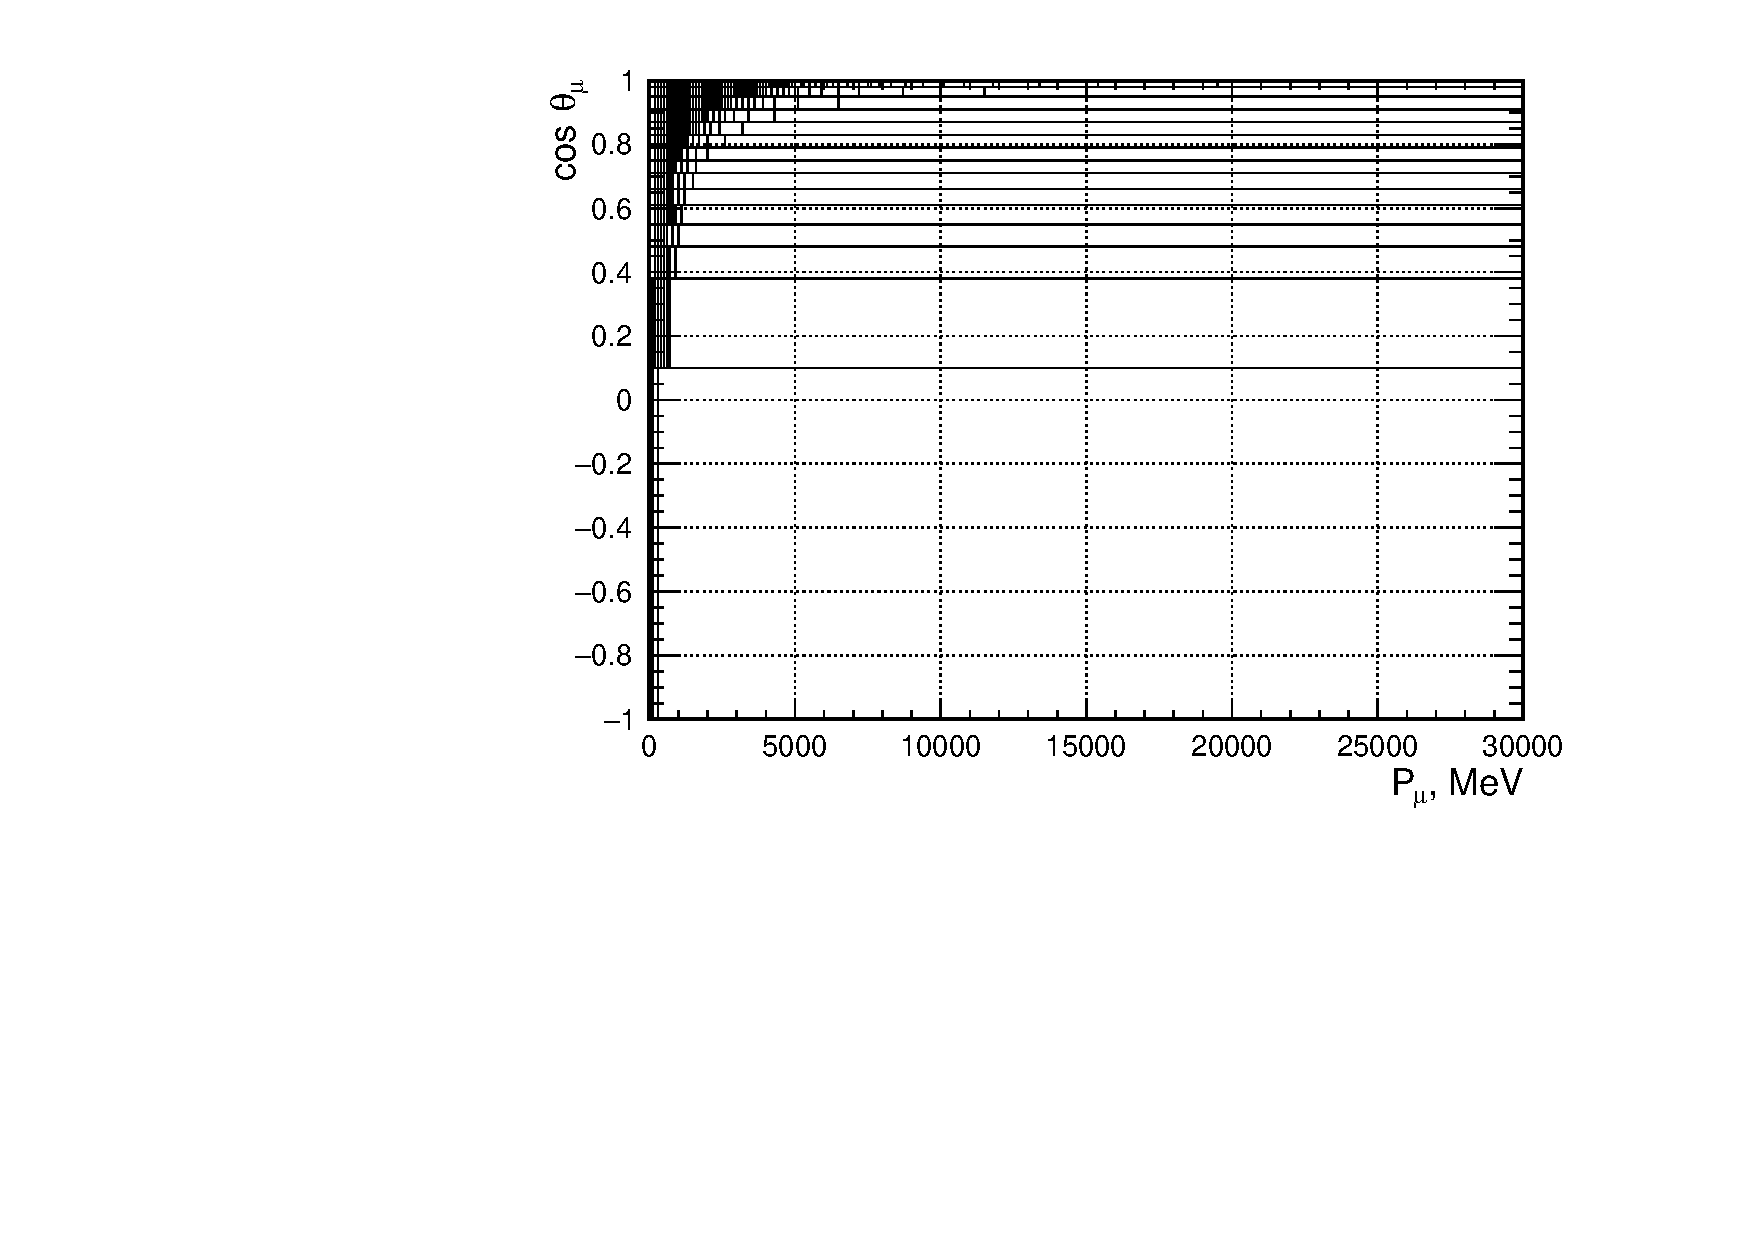
\includegraphics[width=0.95\linewidth]{figs/TH2PolyReset_MC_FGD1_numuCC_1pi}
  \caption{FGD1 FHC $\nu_{\mu}$ 1$\pi$}
  \label{fig:TH2Poly_ResetFGD1_numuCC_1pi}
\end{subfigure}
\begin{subfigure}{.32\textwidth}
  \centering
  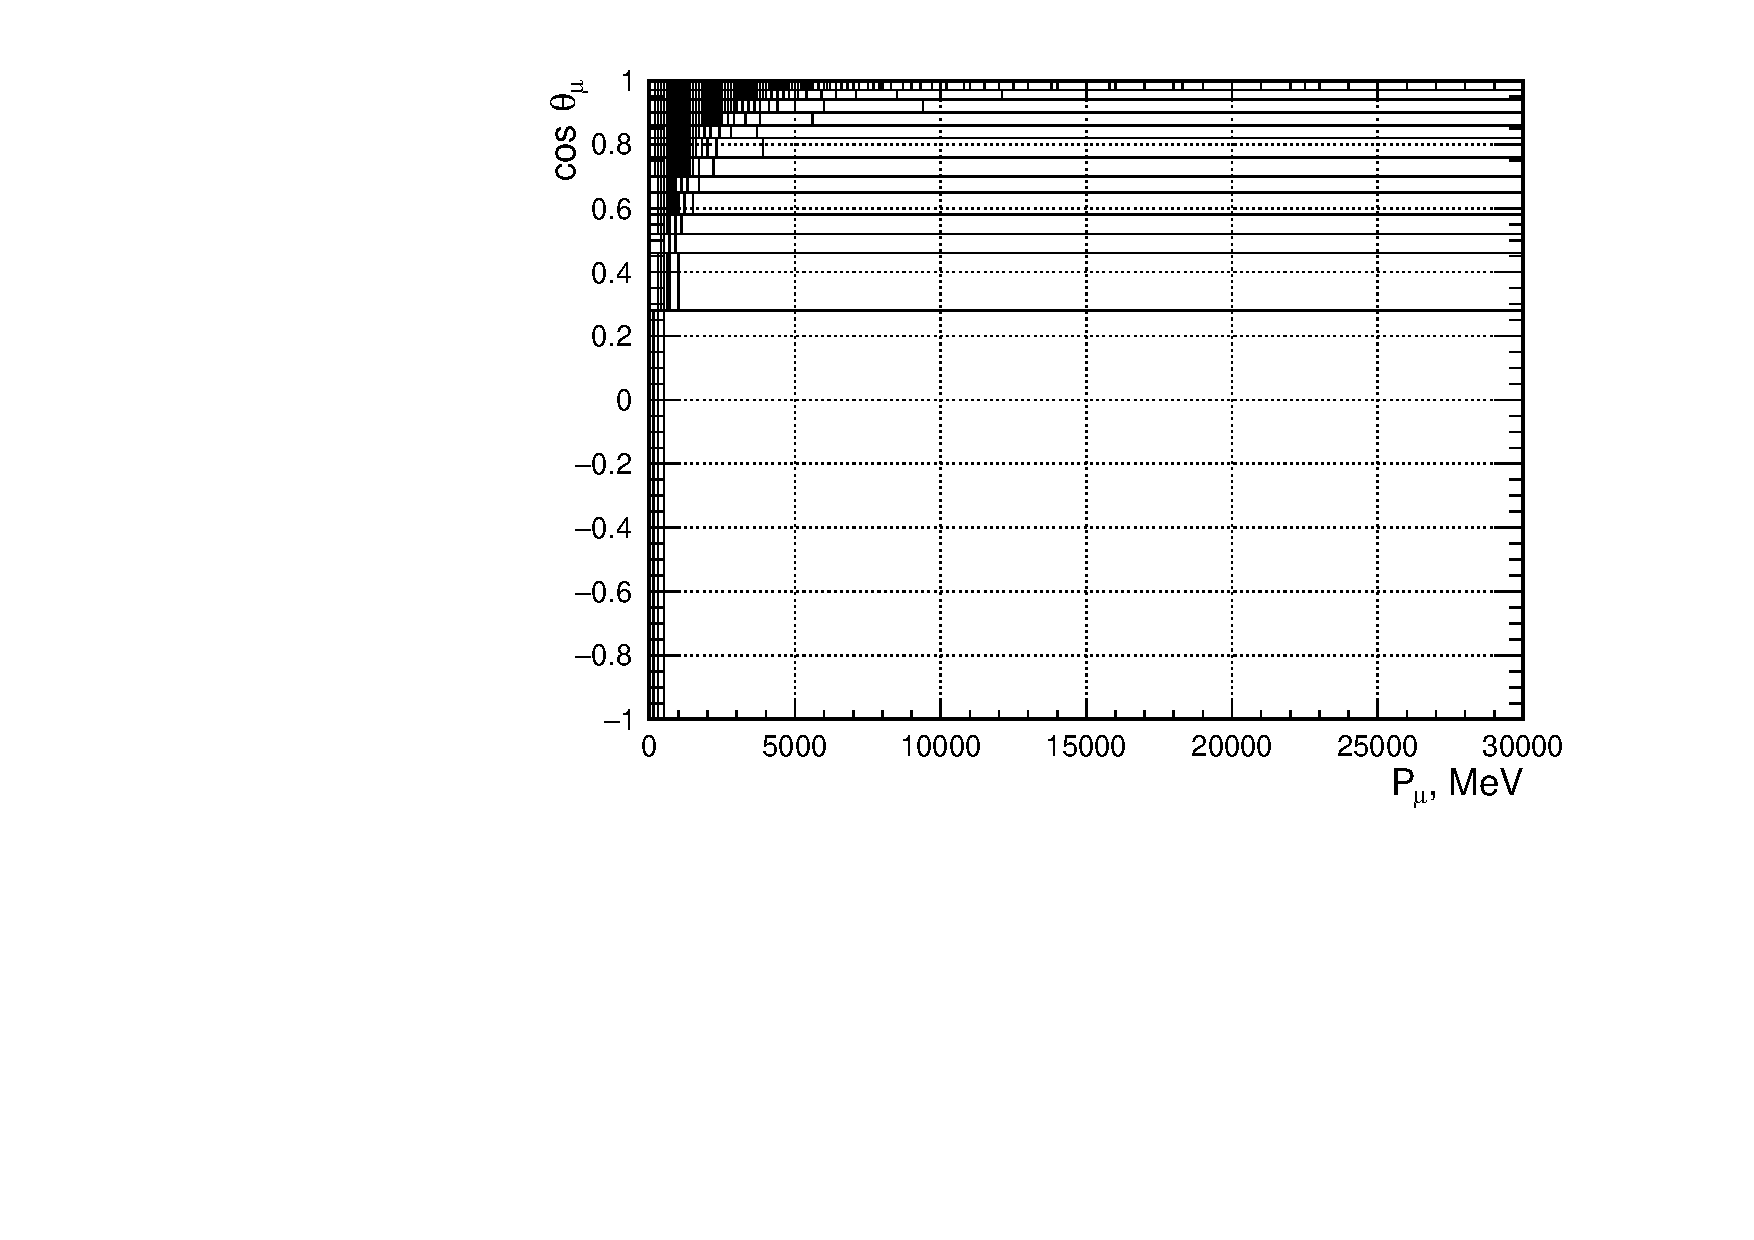
\includegraphics[width=0.95\linewidth]{figs/TH2PolyReset_MC_FGD1_numuCC_other}
  \caption{FGD1 FHC $\nu_{\mu}$ Other}
  \label{fig:TH2Poly_ResetFGD1_numuCC_other}
\end{subfigure}
\centering
\begin{subfigure}{.32\textwidth}
  \centering
  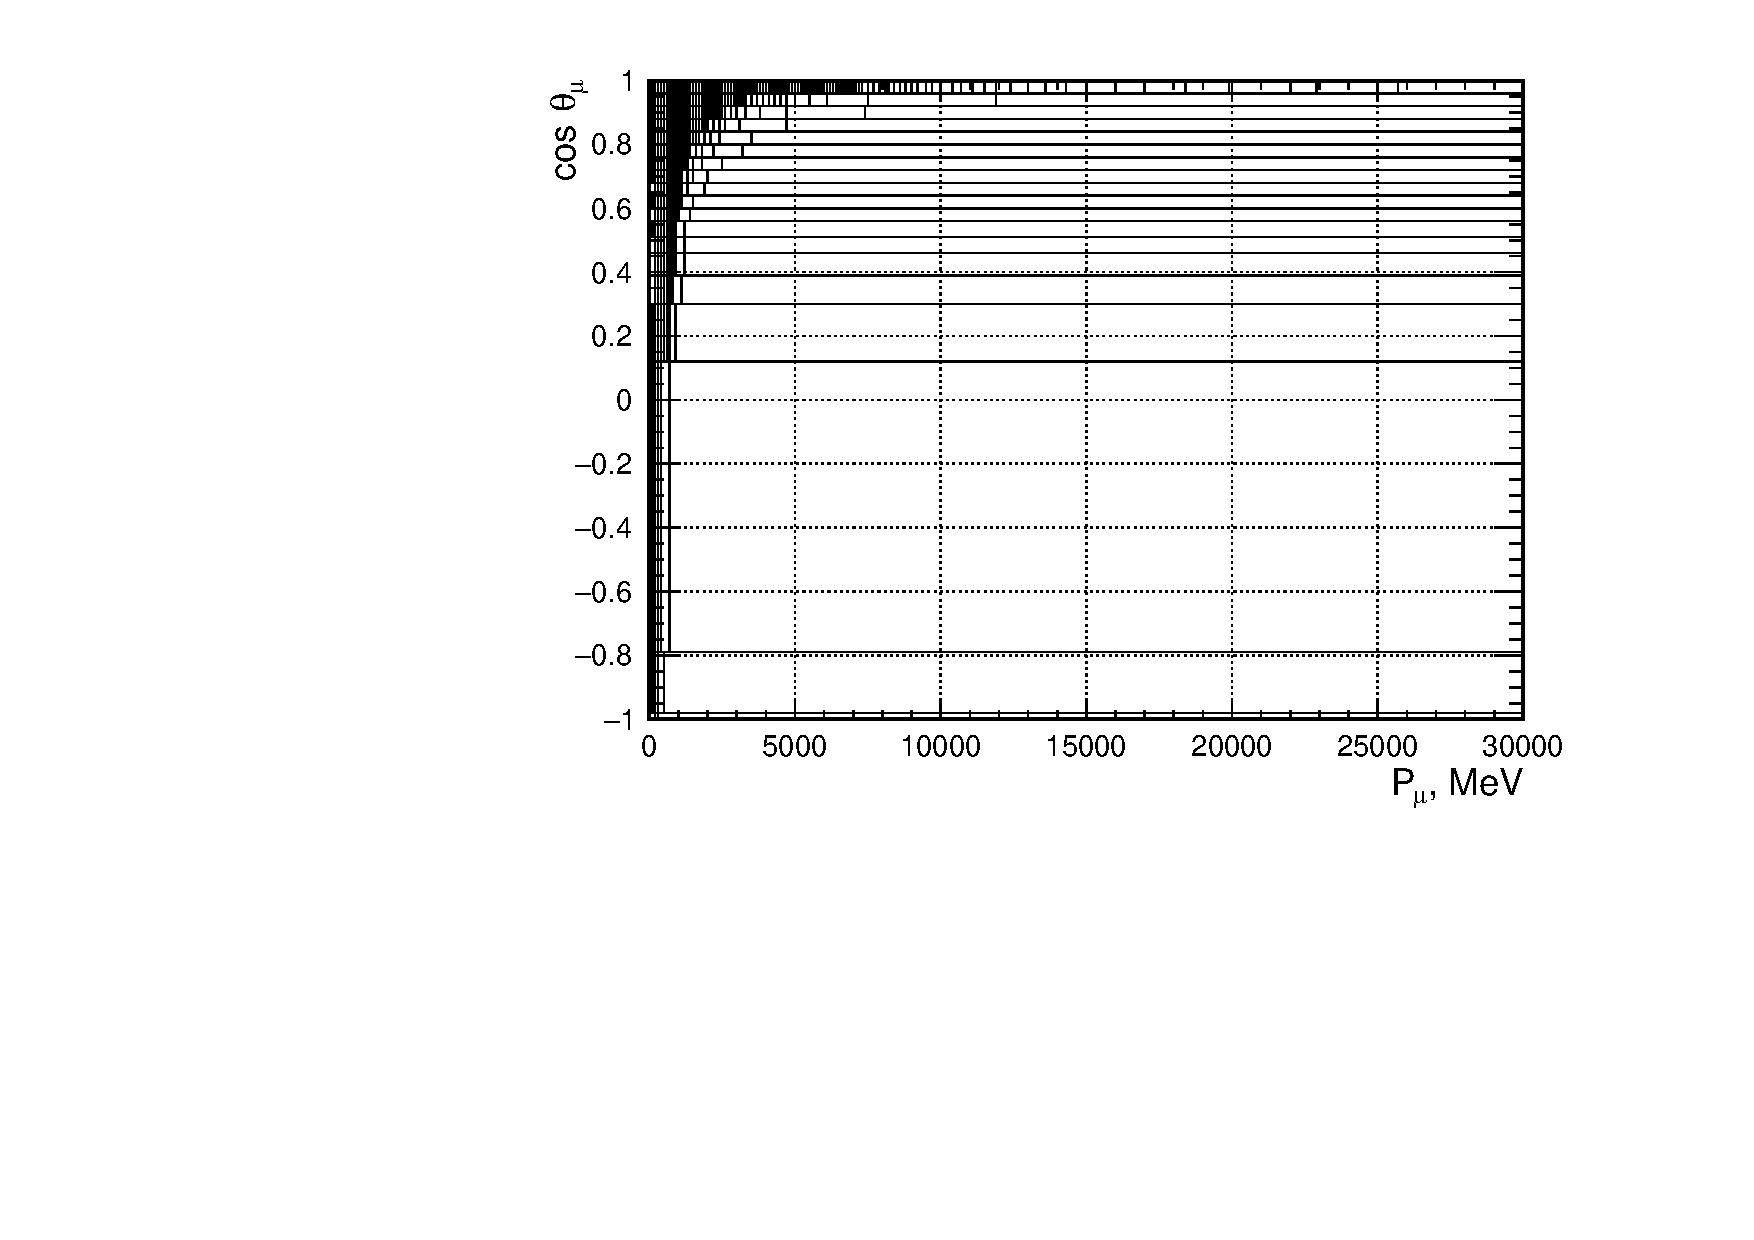
\includegraphics[width=0.95\linewidth]{figs/TH2PolyReset_MC_FGD2_numuCC_0pi}
  \caption{FGD2 FHC $\nu_{\mu}$ 0$\pi$}
  \label{fig:TH2Poly_ResetFGD2_numuCC_0pi}
\end{subfigure}
\begin{subfigure}{.32\textwidth}
  \centering
  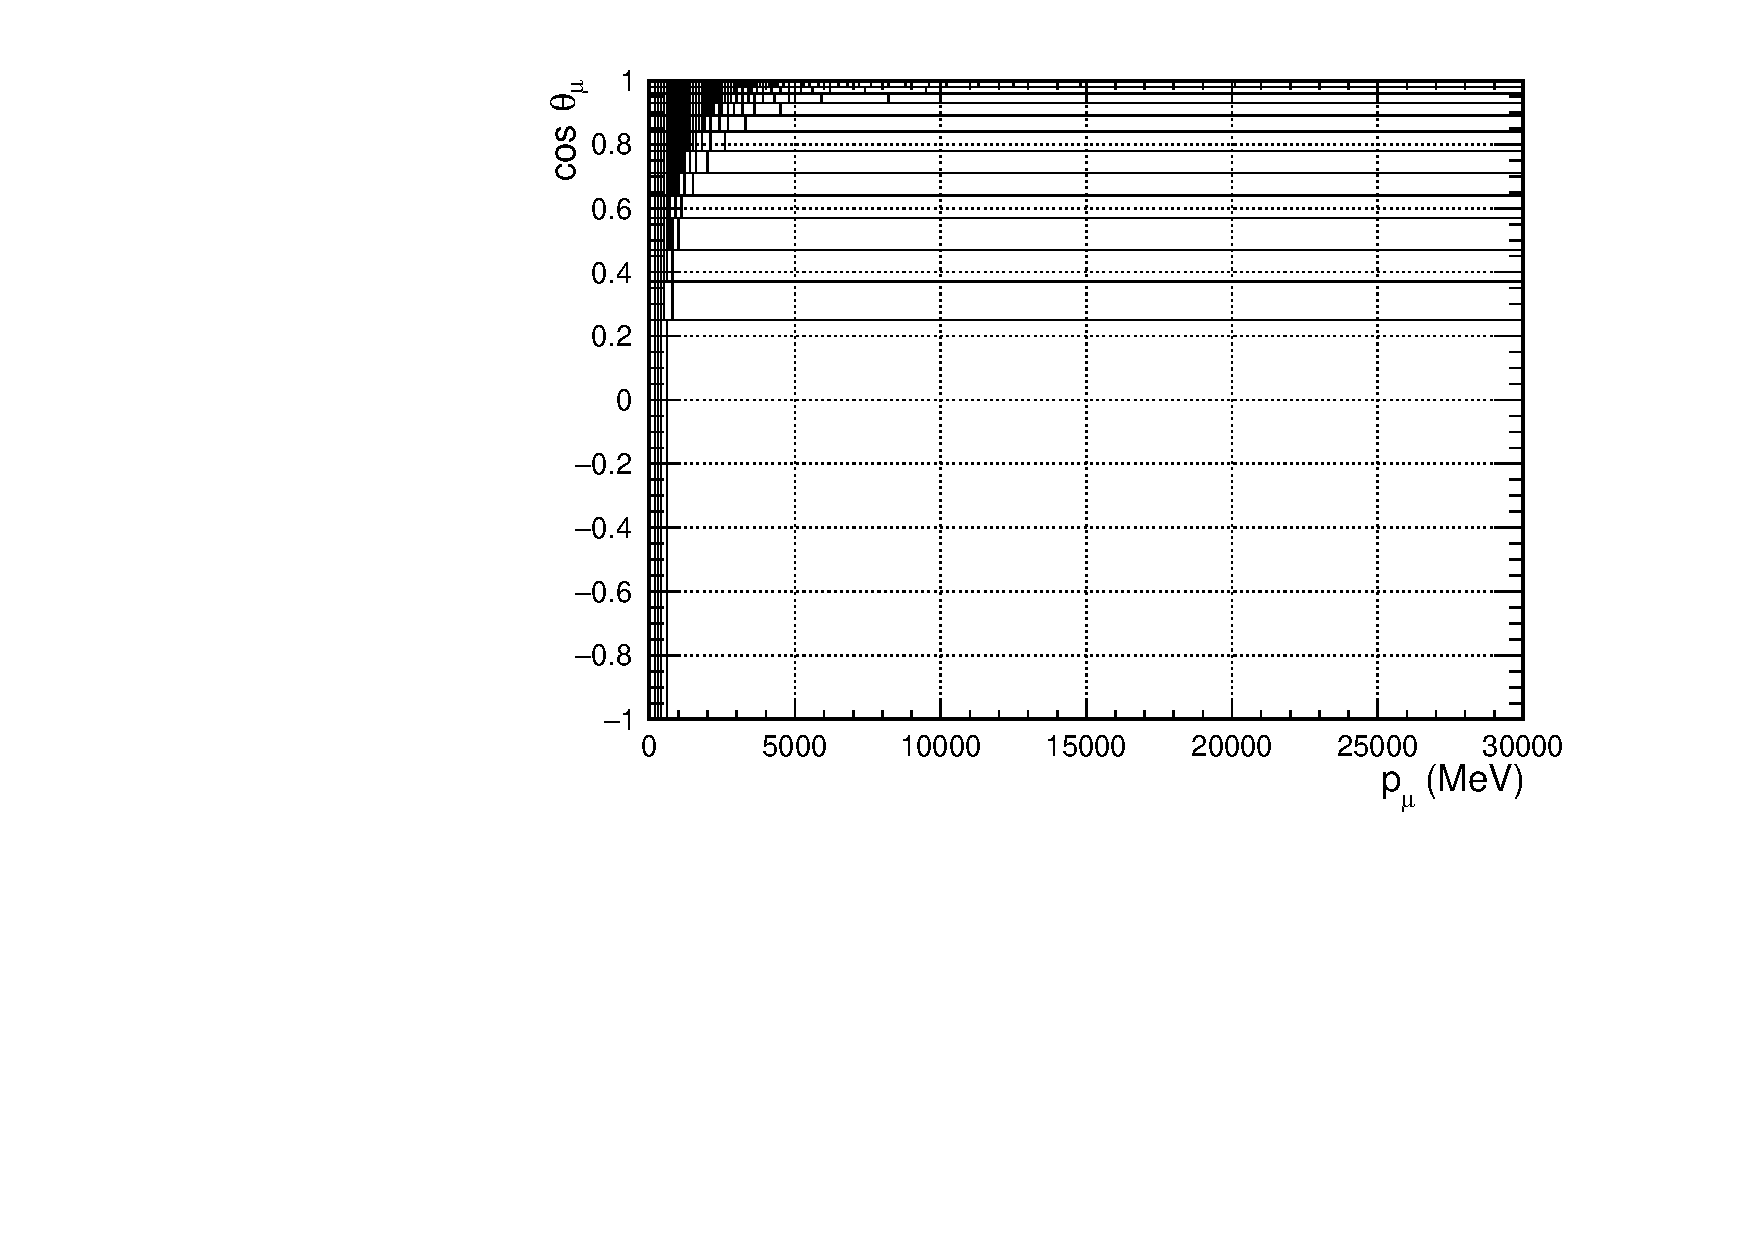
\includegraphics[width=0.95\linewidth]{figs/TH2PolyReset_MC_FGD2_numuCC_1pi}
  \caption{FGD2 FHC $\nu_{\mu}$ 1$\pi$}
  \label{fig:TH2Poly_ResetFGD2_numuCC_1pi}
\end{subfigure}
\begin{subfigure}{.32\textwidth}
  \centering
  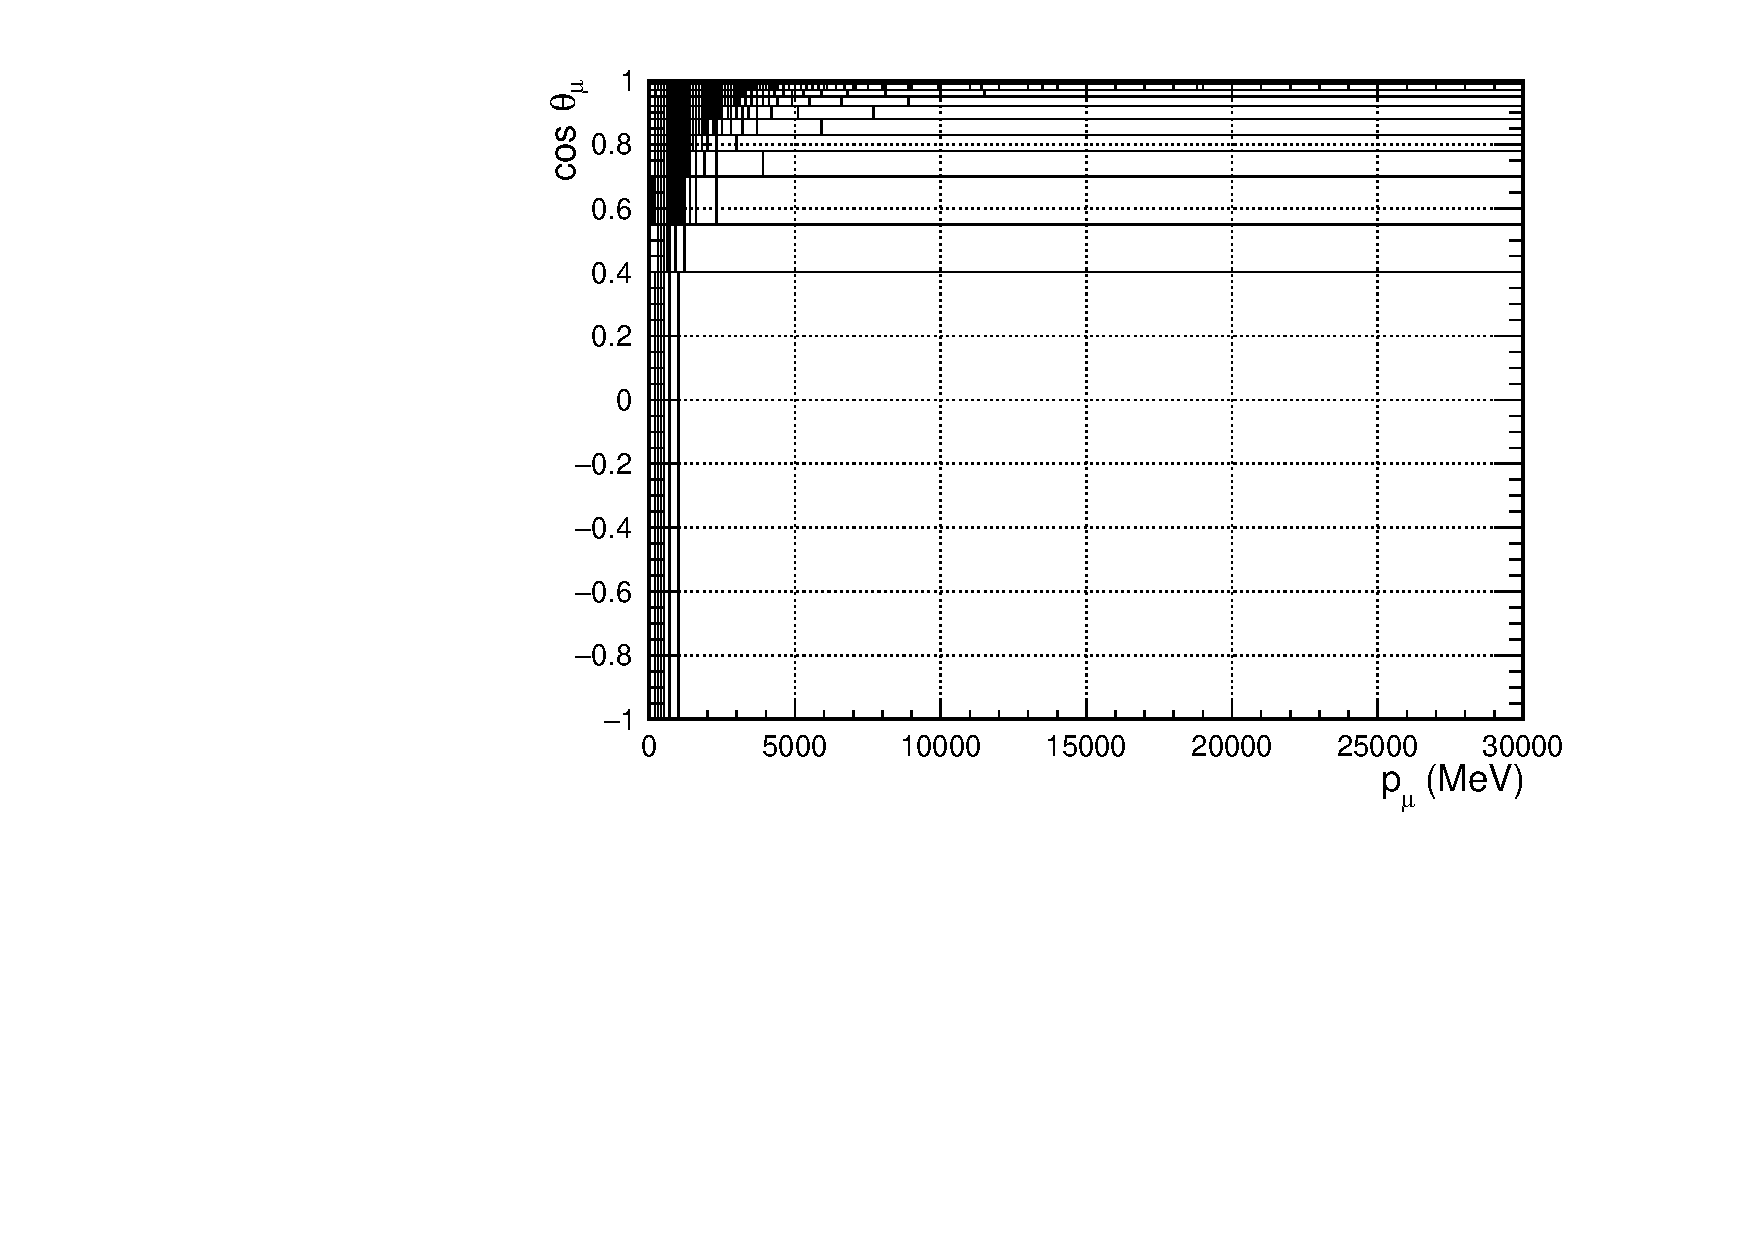
\includegraphics[width=0.95\linewidth]{figs/TH2PolyReset_MC_FGD2_numuCC_other}
  \caption{FGD2 FHC $\nu_{\mu}$ Other}
  \label{fig:TH2Poly_ResetFGD2_numuCC_other}
\end{subfigure}
\centering
\begin{subfigure}{.32\textwidth}
  \centering
  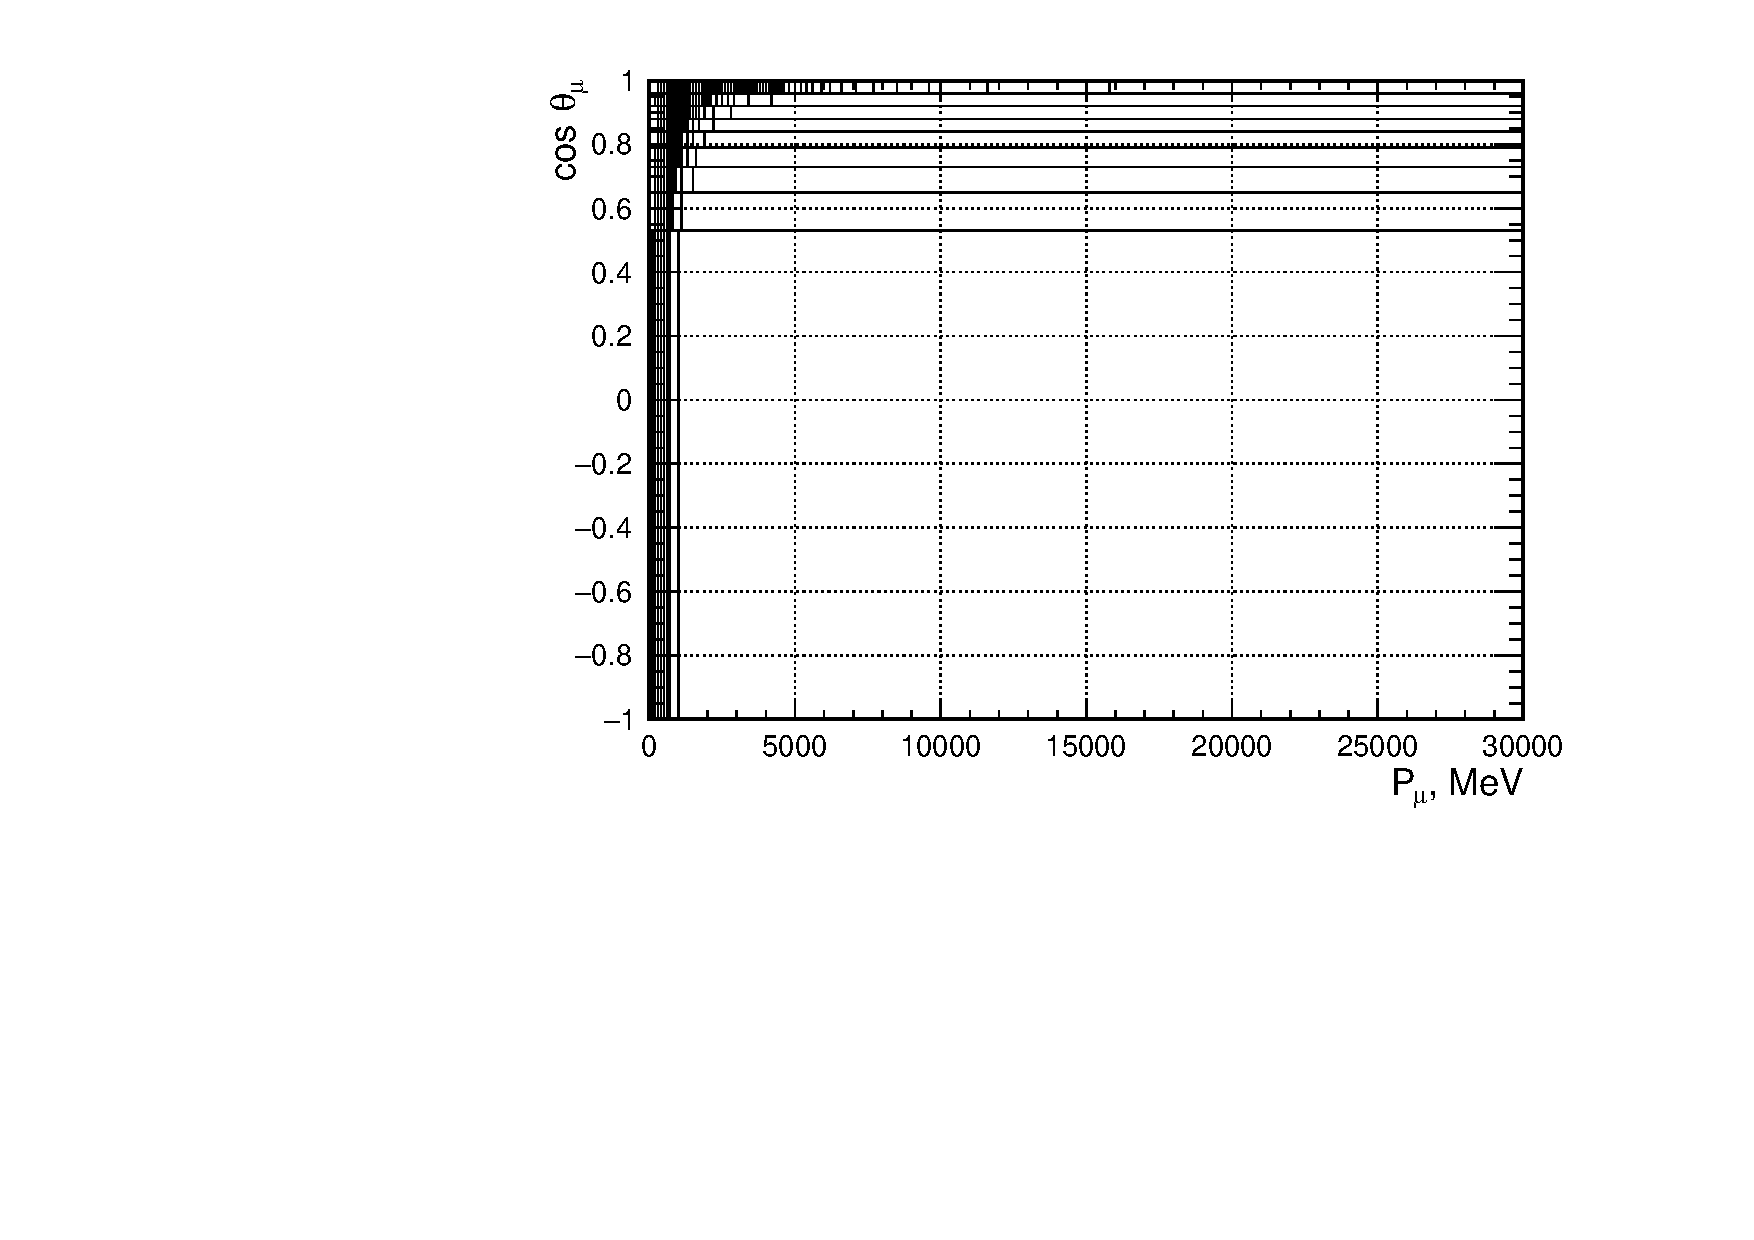
\includegraphics[width=0.95\linewidth]{figs/TH2PolyReset_MC_FGD1_anti-numuCC_0pi}
  \caption{FGD1 RHC $\bar{\nu_{\mu}}$ 0$\pi$}
  \label{fig:TH2Poly_ResetFGD1_anti-numuCC_0pi}
\end{subfigure}
\begin{subfigure}{.32\textwidth}
  \centering
  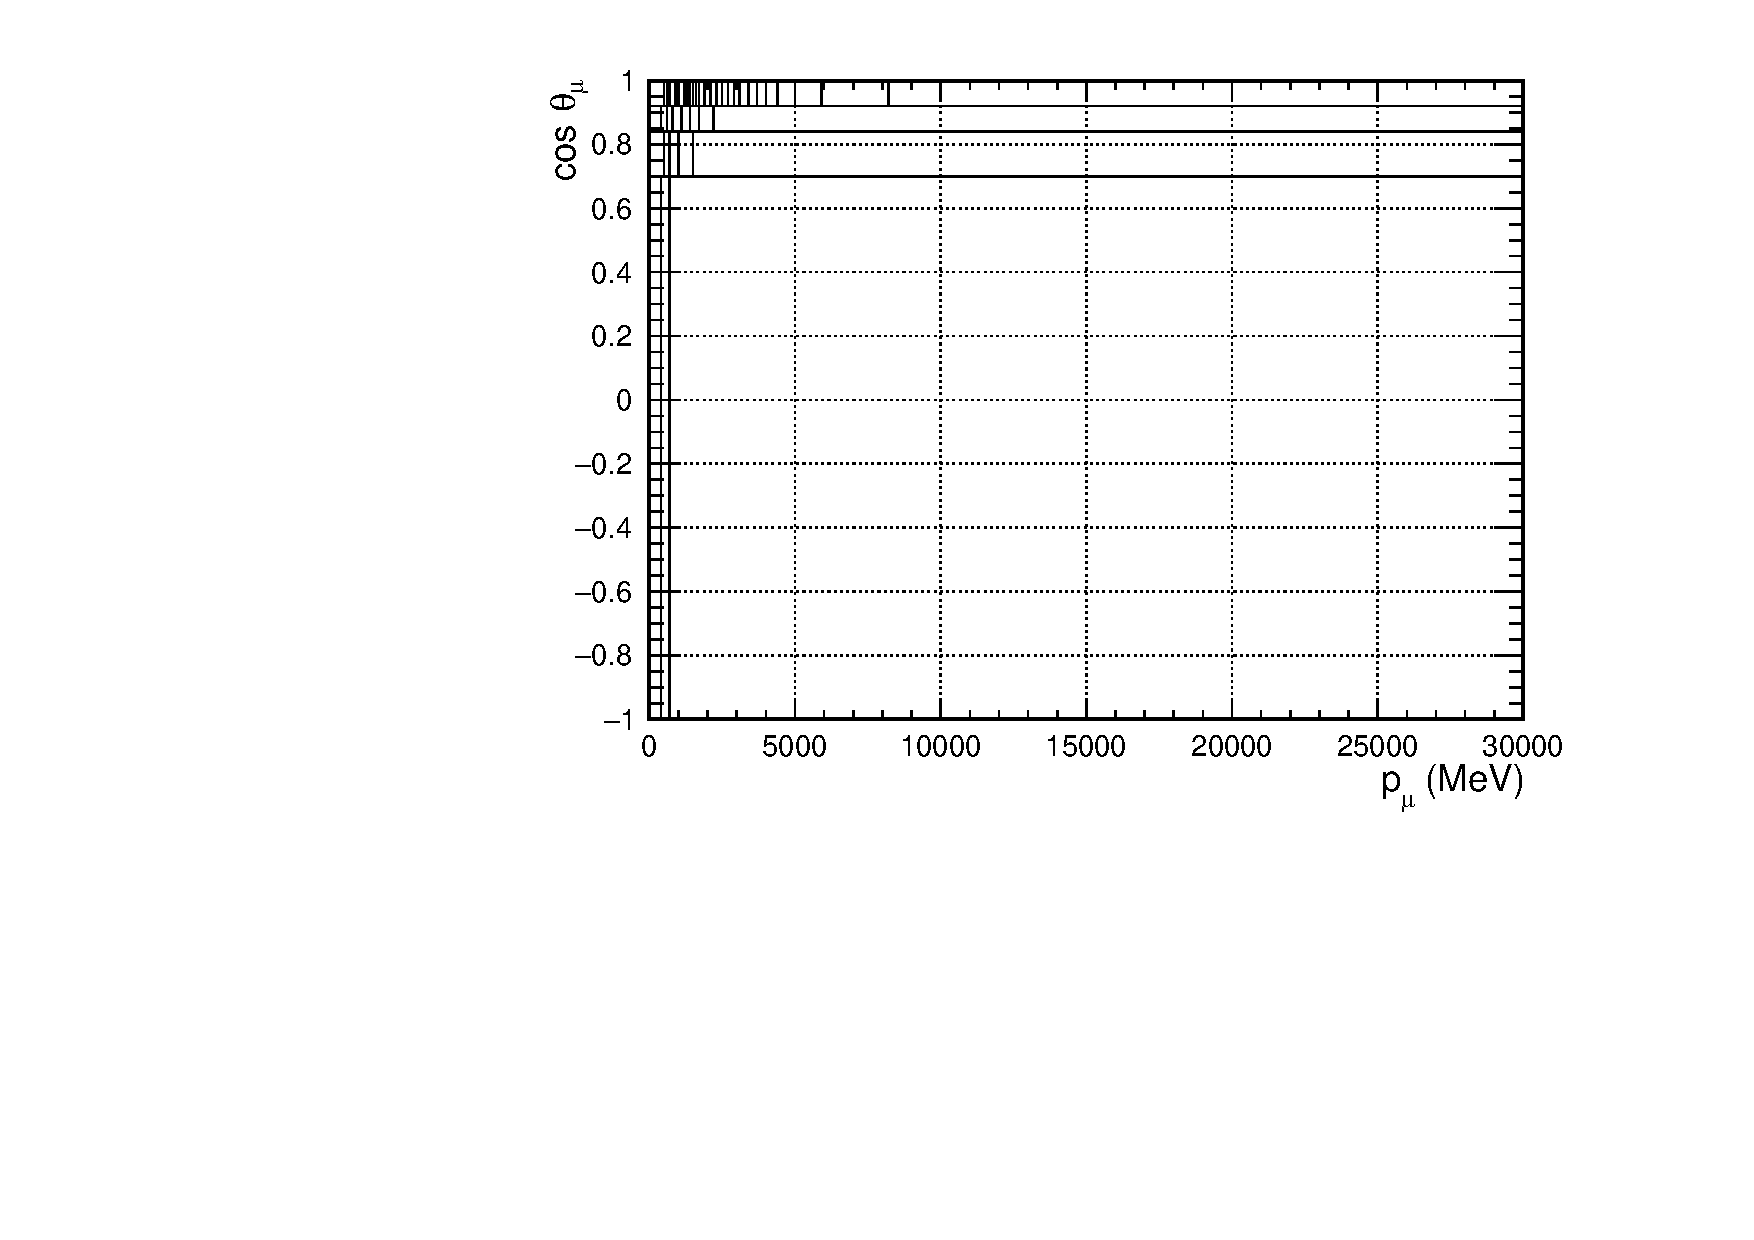
\includegraphics[width=0.95\linewidth]{figs/TH2PolyReset_MC_FGD1_anti-numuCC_1pi}
  \caption{FGD1 RHC $\bar{\nu_{\mu}}$ 1$\pi$}
  \label{fig:th2polyTH2Poly_ResetFGD1_anti-numuCC_1pi}
\end{subfigure}
\begin{subfigure}{.32\textwidth}
  \centering
  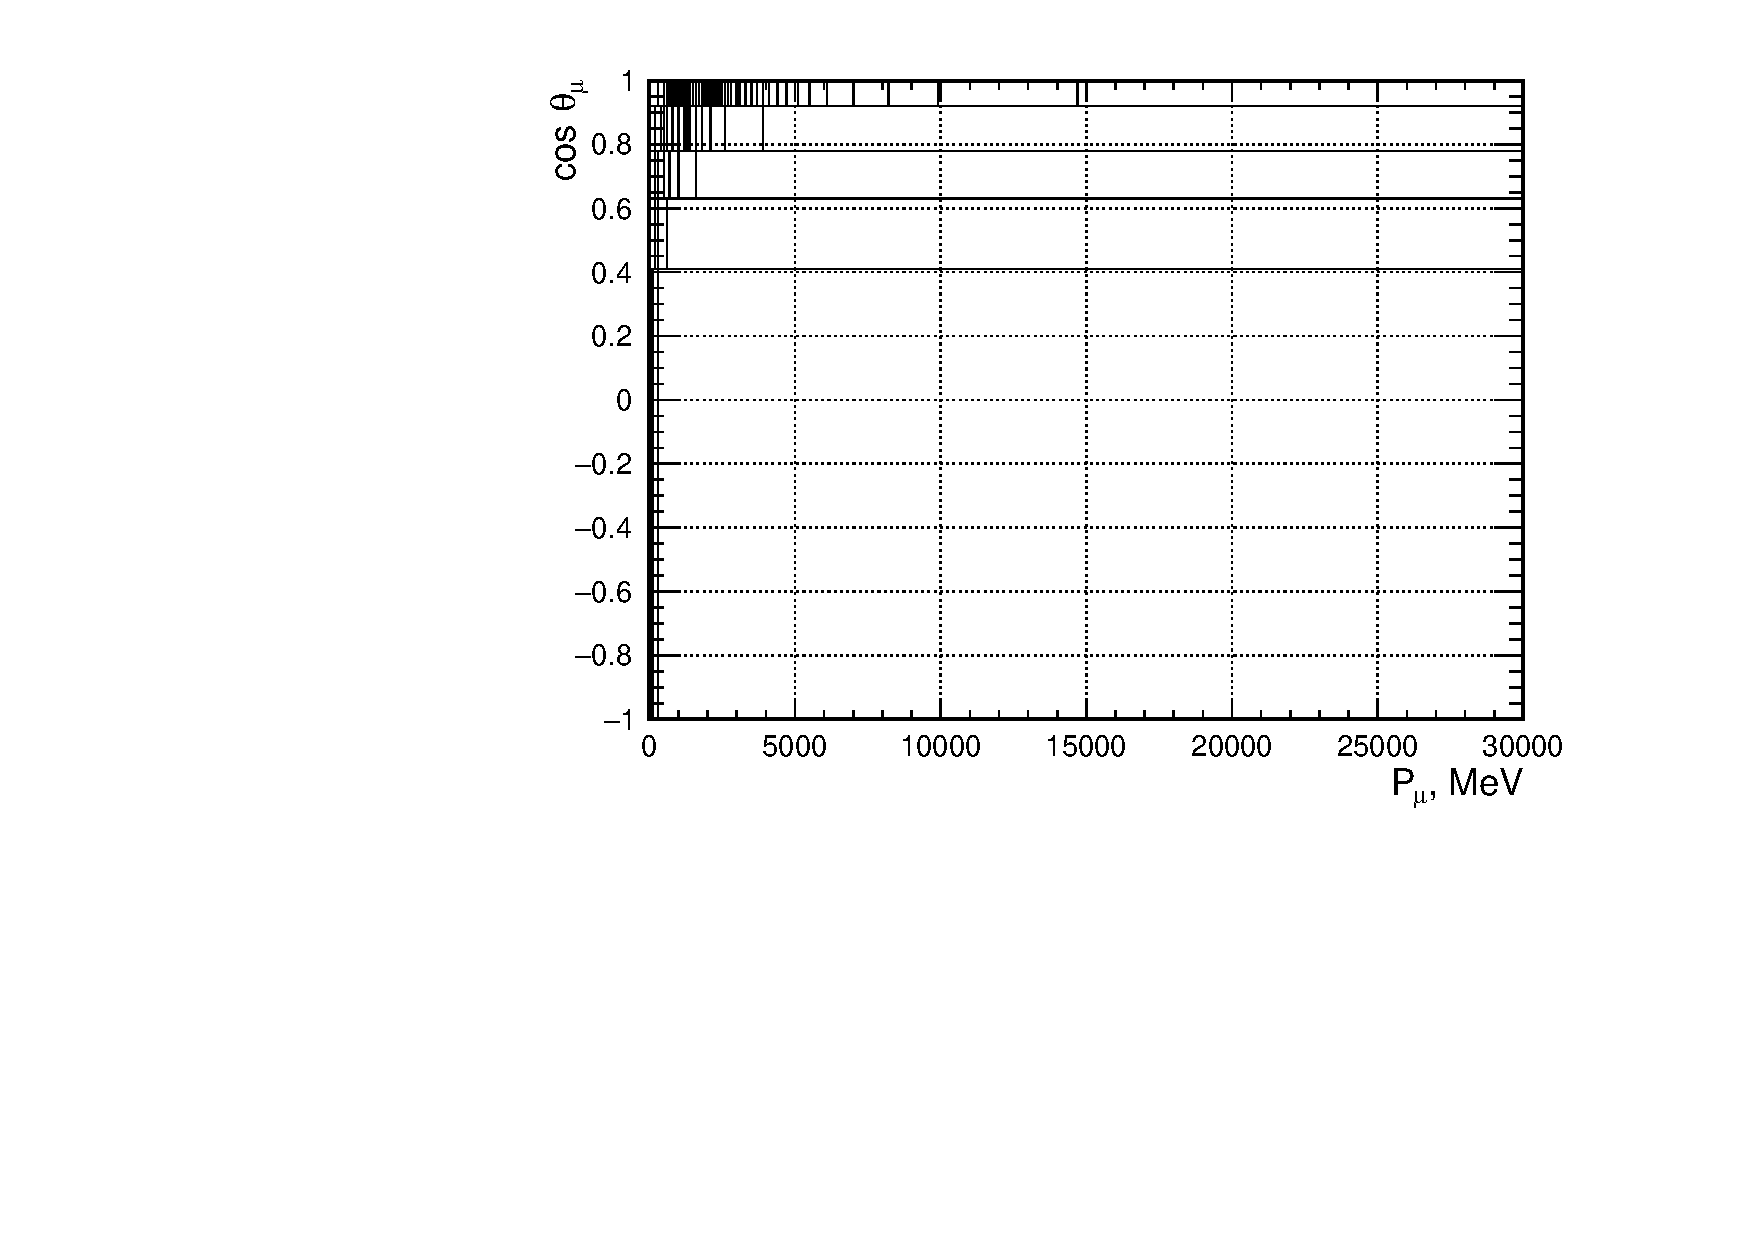
\includegraphics[width=0.95\linewidth]{figs/TH2PolyReset_MC_FGD1_anti-numuCC_other}
  \caption{FGD1 RHC $\bar{\nu_{\mu}}$ Other}
  \label{fig:TH2Poly_ResetFGD1_anti-numuCC_other}
\end{subfigure}
\centering
\begin{subfigure}{.32\textwidth}
  \centering
  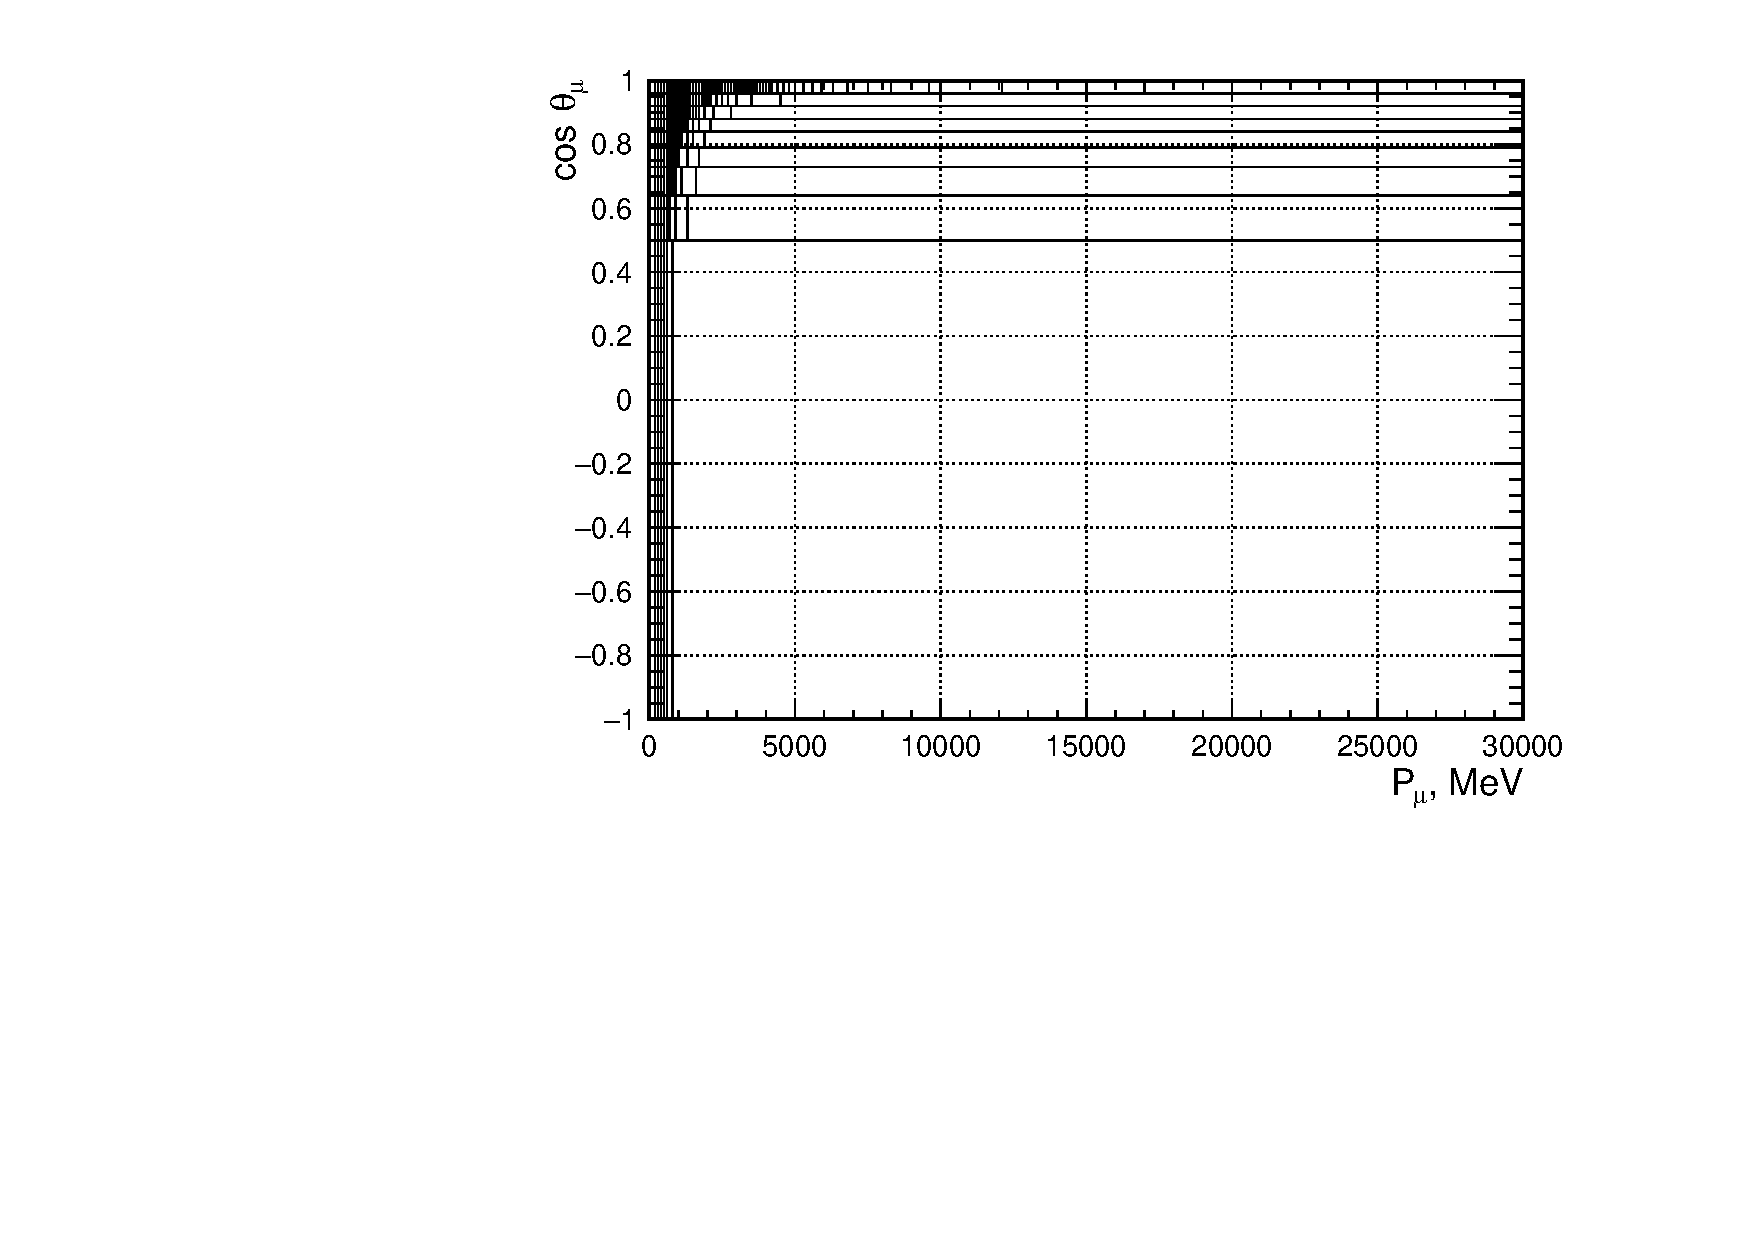
\includegraphics[width=0.95\linewidth]{figs/TH2PolyReset_MC_FGD2_anti-numuCC_0pi}
  \caption{FGD2 RHC $\bar{\nu_{\mu}}$ 0$\pi$}
  \label{fig:TH2Poly_ResetFGD2_anti-numuCC_0pi}
\end{subfigure}
\begin{subfigure}{.32\textwidth}
  \centering
  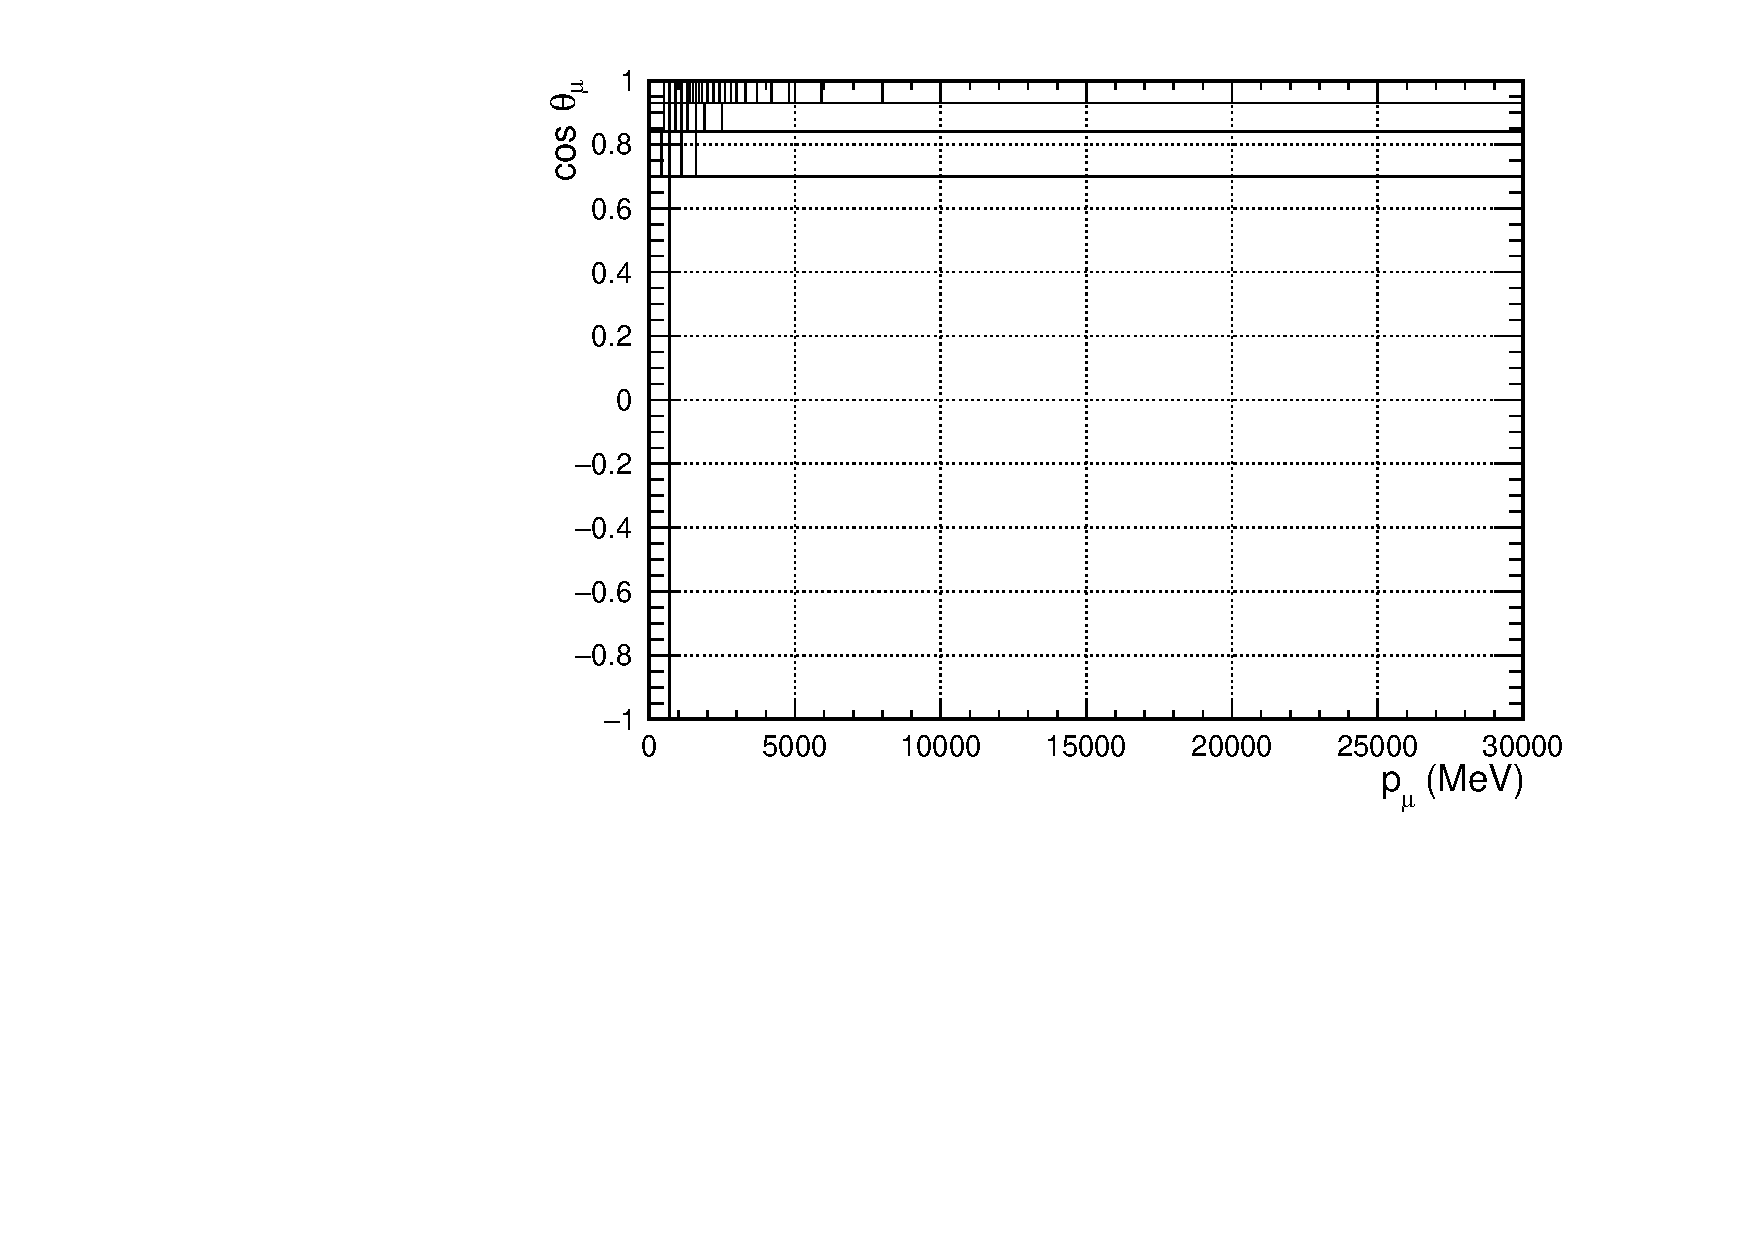
\includegraphics[width=0.95\linewidth]{figs/TH2PolyReset_MC_FGD2_anti-numuCC_1pi}
  \caption{FGD2 RHC $\bar{\nu_{\mu}}$ 1$\pi$}
  \label{fig:th2polyTH2Poly_ResetFGD2_anti-numuCC_1pi}
\end{subfigure}
\begin{subfigure}{.32\textwidth}
  \centering
  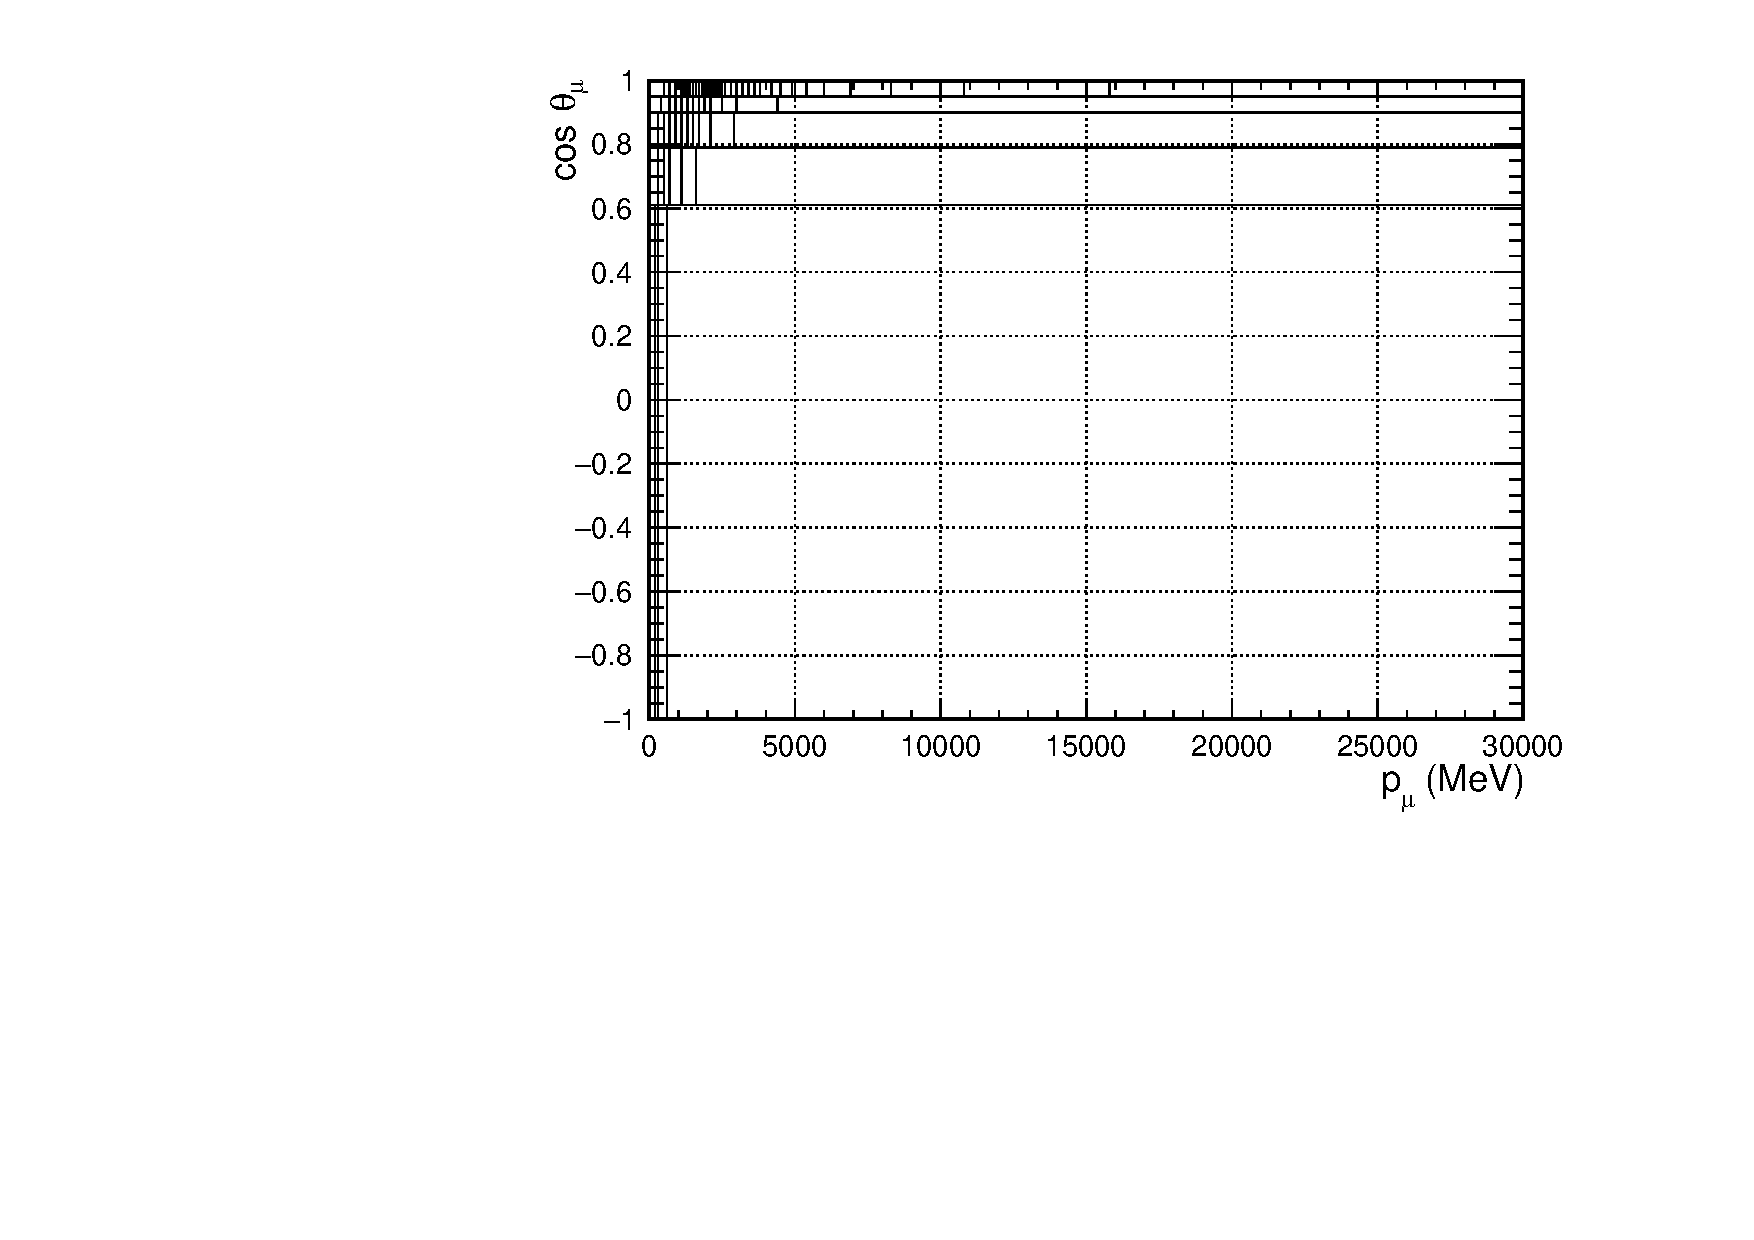
\includegraphics[width=0.95\linewidth]{figs/TH2PolyReset_MC_FGD2_anti-numuCC_other}
  \caption{FGD2 RHC $\bar{\nu_{\mu}}$ Other}
  \label{fig:TH2Poly_ResetFGD2_anti-numuCC_other}
\end{subfigure}
\begin{subfigure}{.32\textwidth}
  \centering
  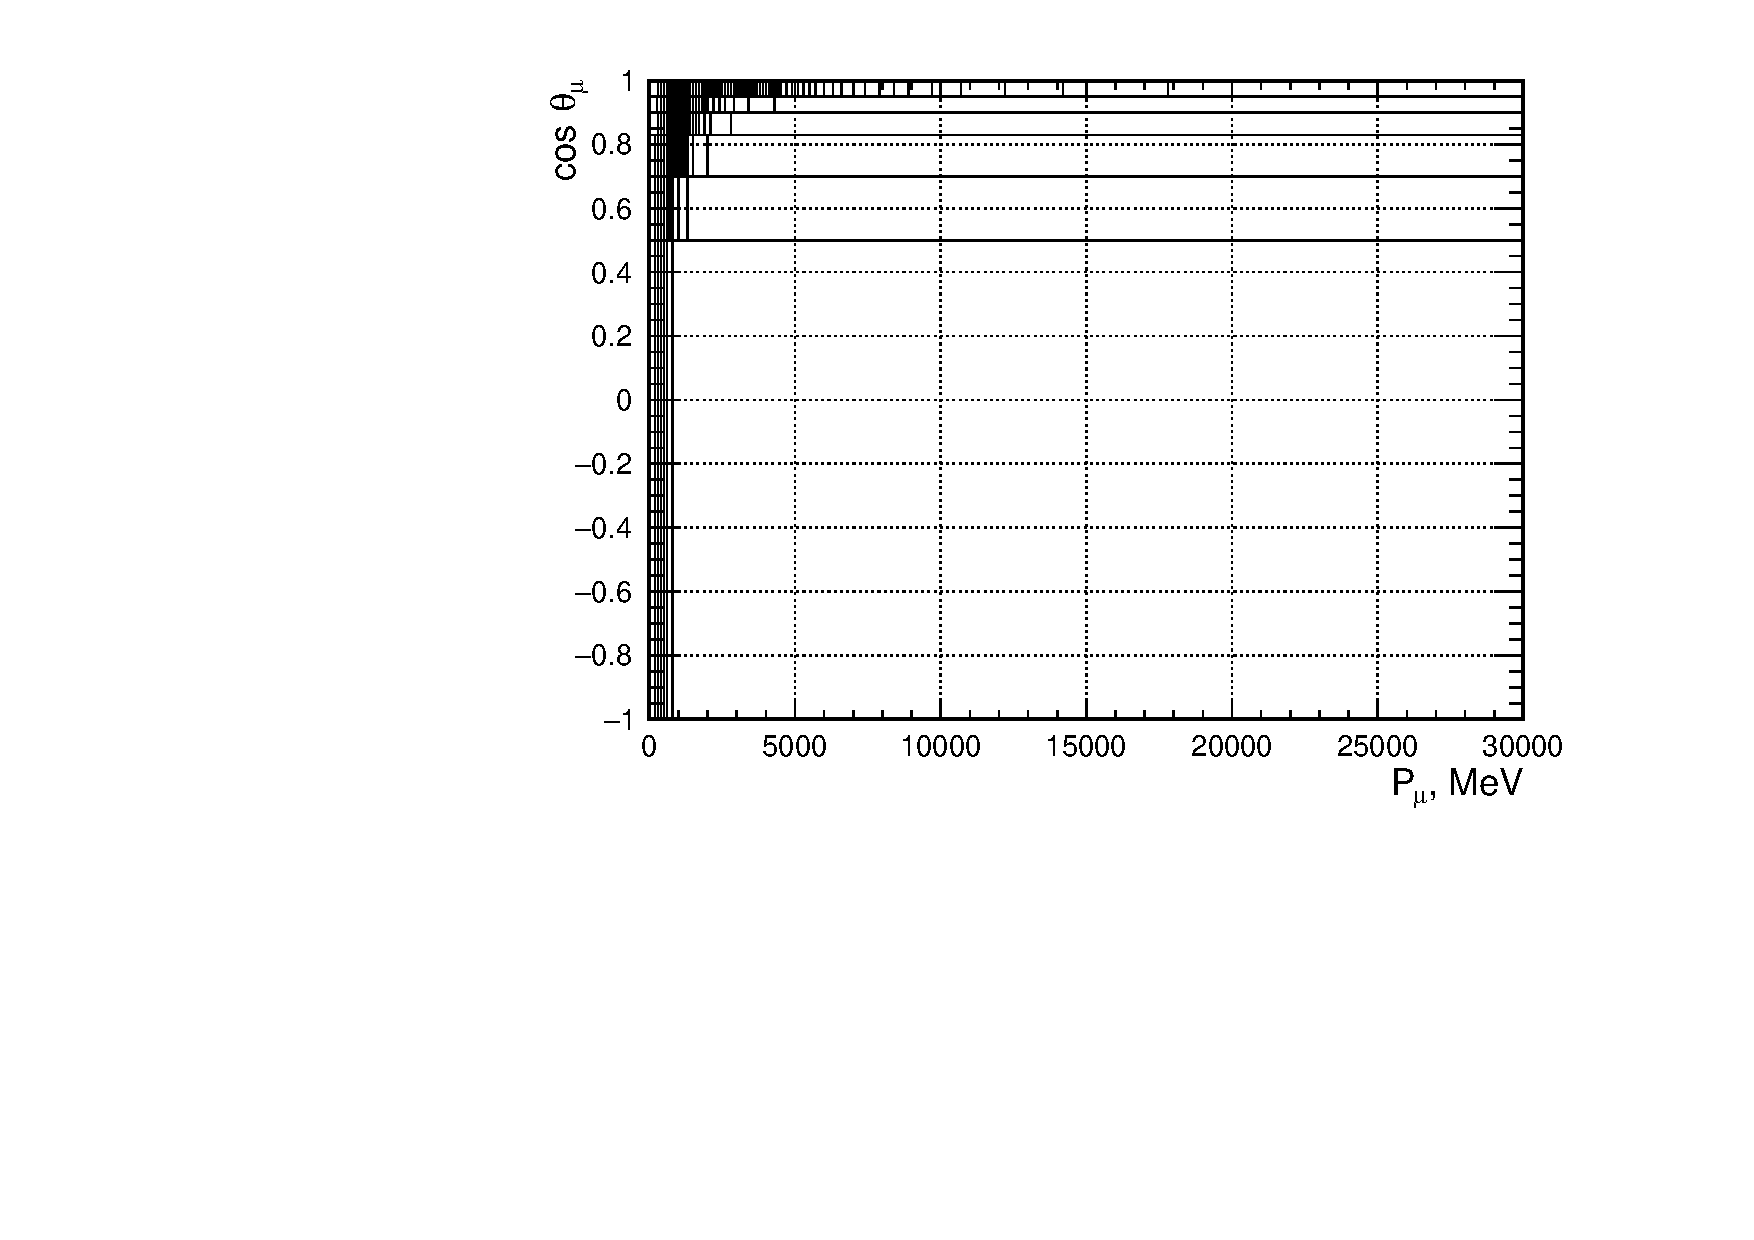
\includegraphics[width=0.95\linewidth]{figs/TH2PolyReset_MC_FGD1_NuMuBkg_CC0pi_in_AntiNu_Mode}
  \caption{FGD1 RHC $\nu_{\mu}$ 0$\pi$}
  \label{fig:TH2Poly_ResetFGD1_NuMuBkg_CC0pi_in_AntiNu_Mode}
\end{subfigure}
\begin{subfigure}{.32\textwidth}
  \centering
  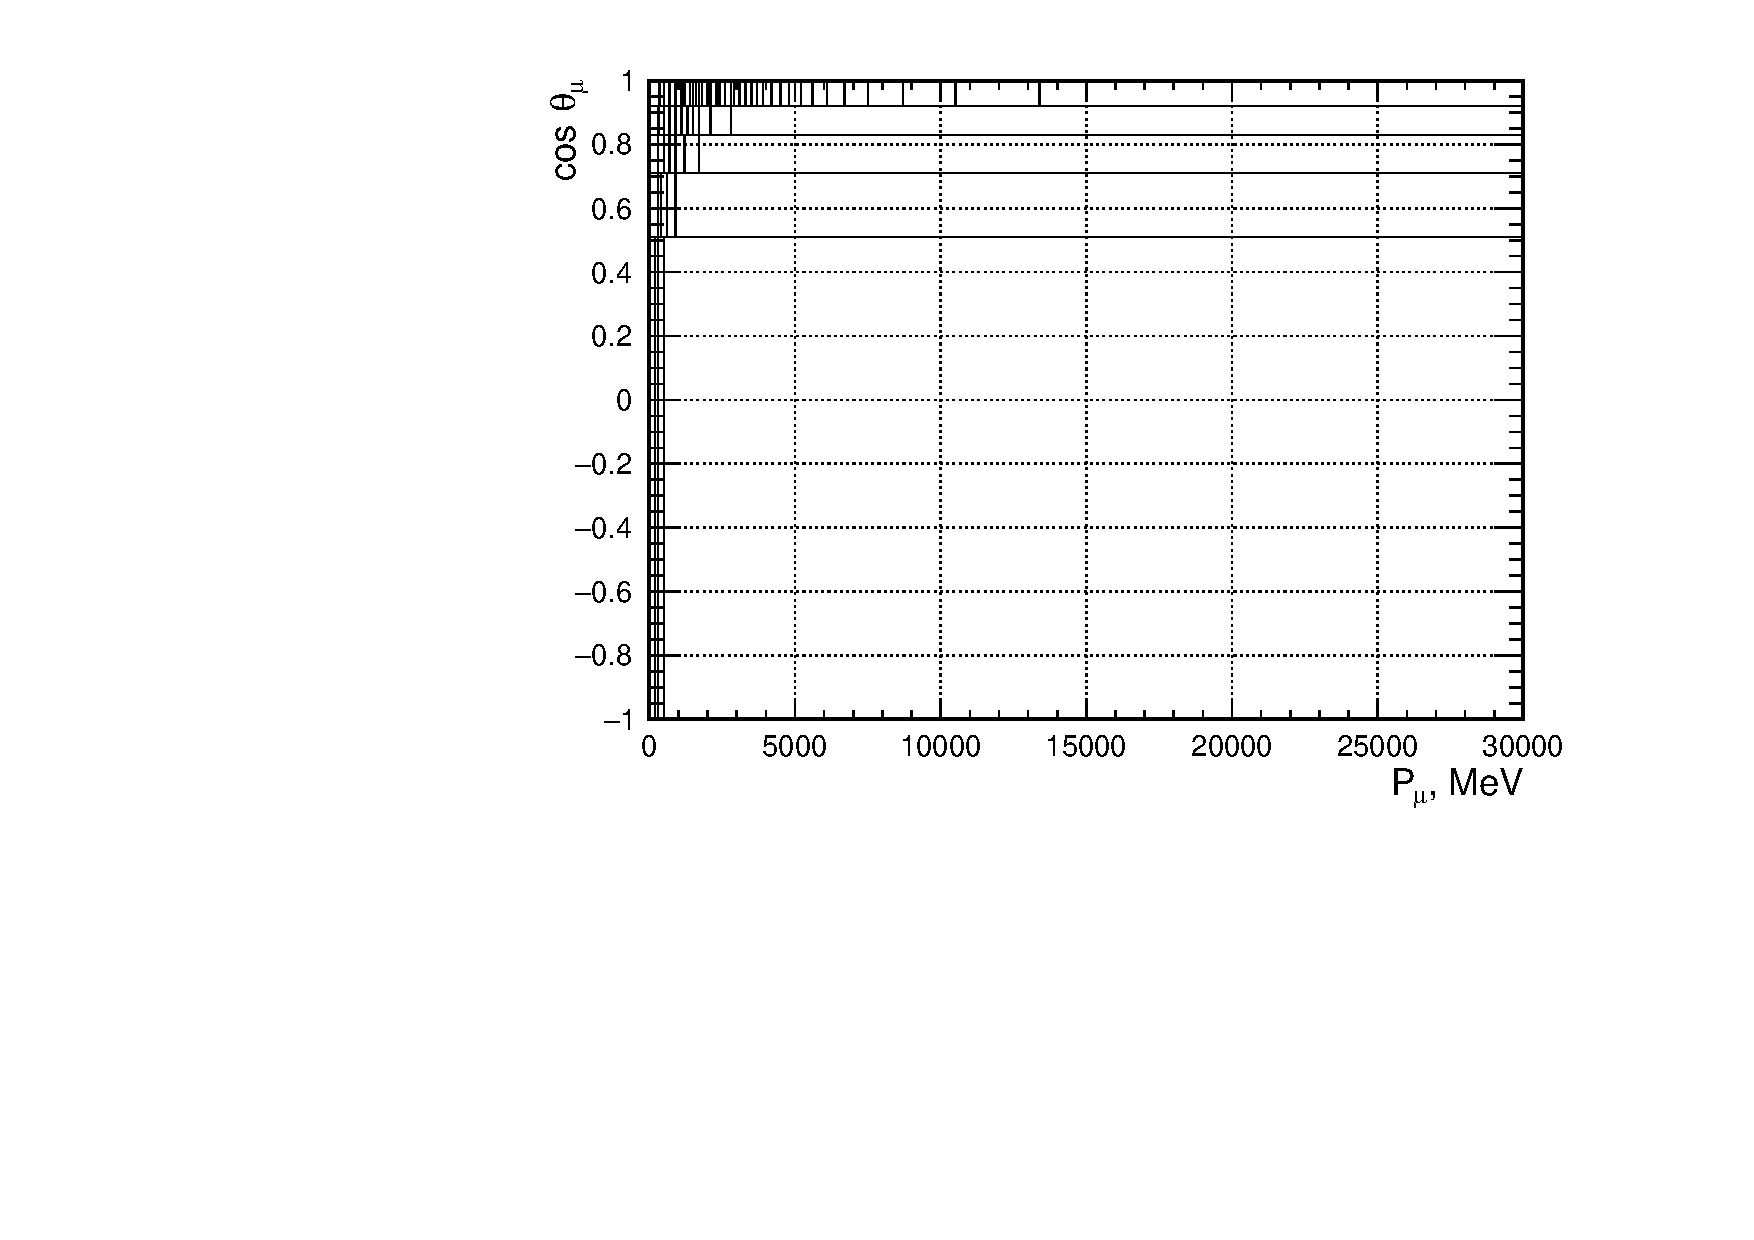
\includegraphics[width=0.95\linewidth]{figs/TH2PolyReset_MC_FGD1_NuMuBkg_CC1pi_in_AntiNu_Mode}
  \caption{FGD1 RHC $\nu_{\mu}$ 1$\pi$}
  \label{fig:TH2Poly_ResetFGD1_NuMuBkg_CC1pi_in_AntiNu_Mode}
\end{subfigure}
\begin{subfigure}{.32\textwidth}
  \centering
  \includegraphics[width=0.95\linewidth]{figs/TH2PolyReset_MC_FGD1_NuMuBkg_CCOther_in_AntiNu_Mode}
  \caption{FGD1 RHC $\nu_{\mu}$ Other}
  \label{fig:TH2Poly_ResetFGD1_NuMuBkg_CCOther_in_AntiNu_Mode}
\end{subfigure}
\begin{subfigure}{.32\textwidth}
  \centering
  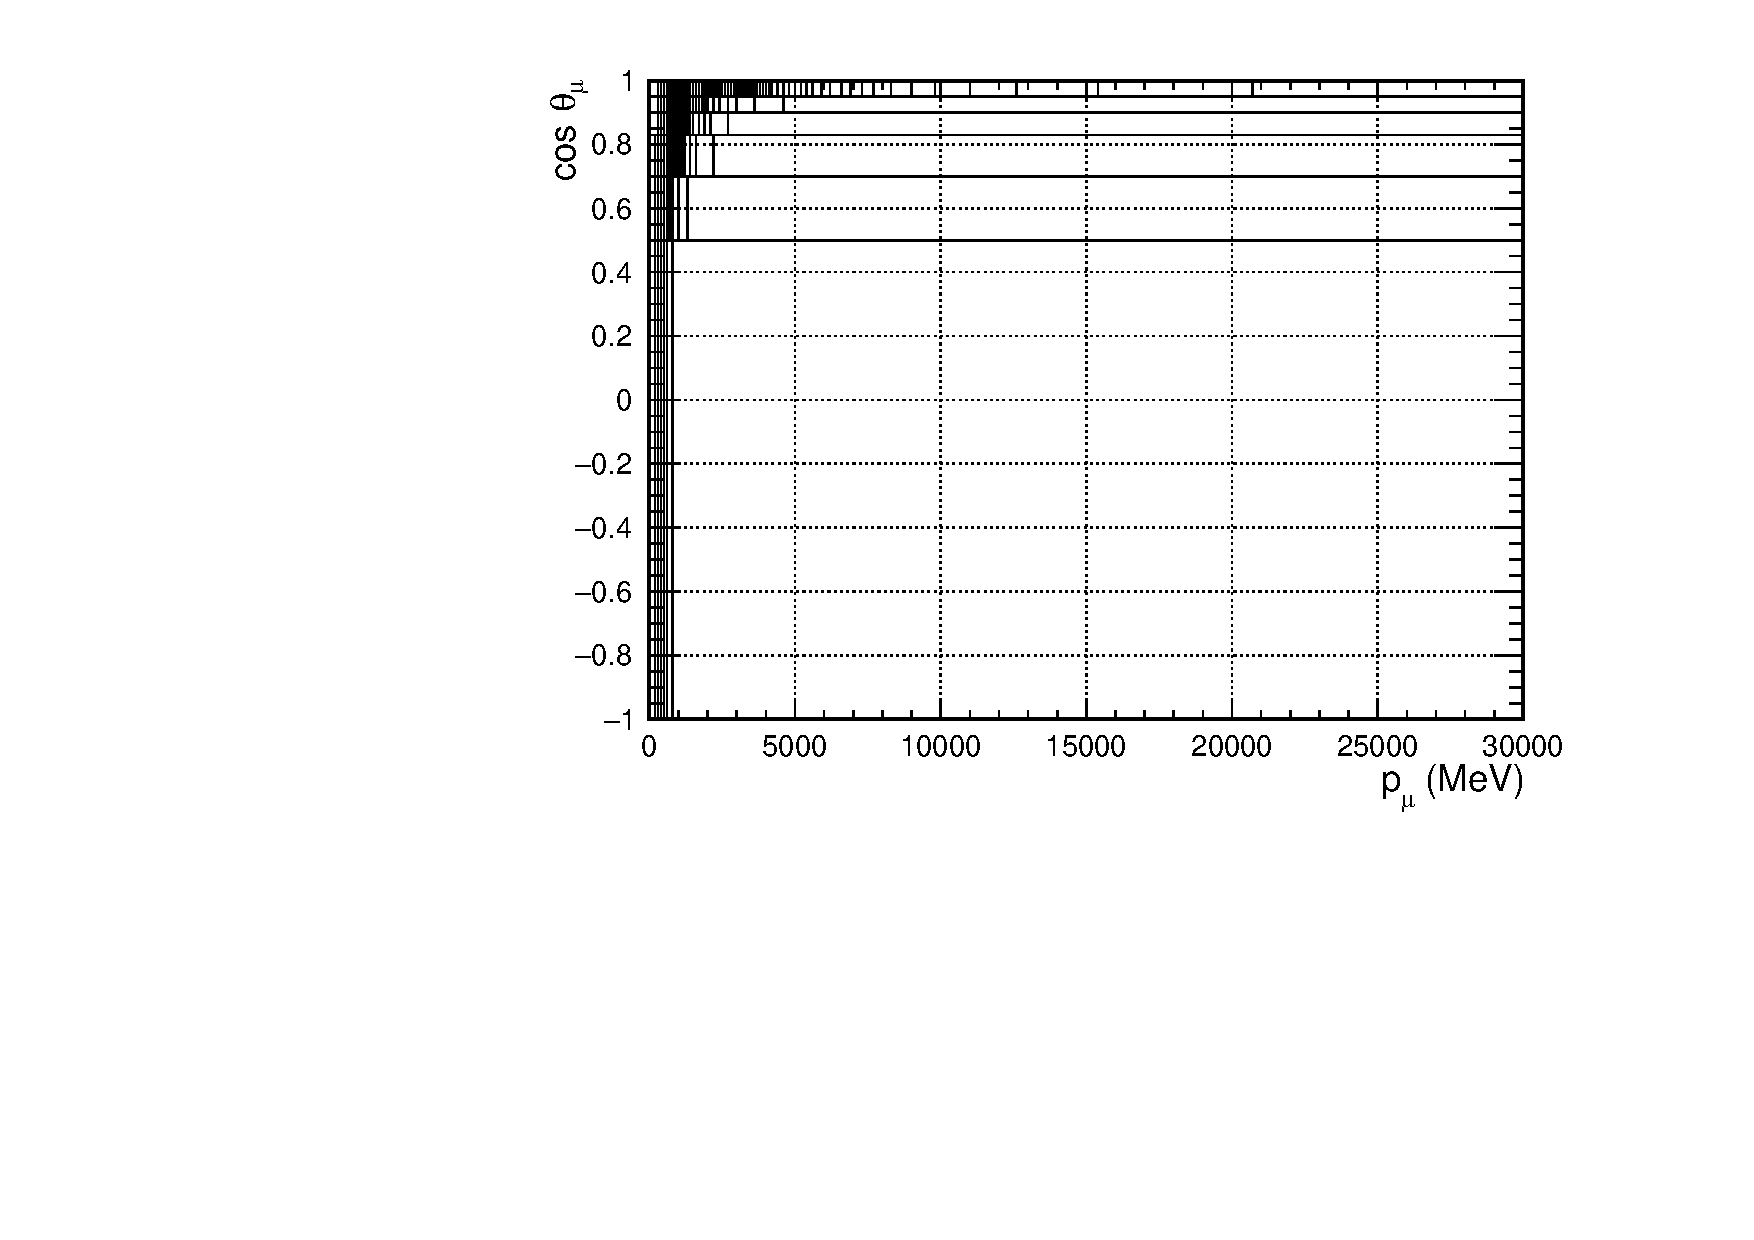
\includegraphics[width=0.95\linewidth]{figs/TH2PolyReset_MC_FGD2_NuMuBkg_CC0pi_in_AntiNu_Mode}
  \caption{FGD2 RHC $\nu_{\mu}$ 0$\pi$}
  \label{fig:TH2Poly_ResetFGD2_NuMuBkg_CC0pi_in_AntiNu_Mode}
\end{subfigure}
\begin{subfigure}{.32\textwidth}
  \centering
  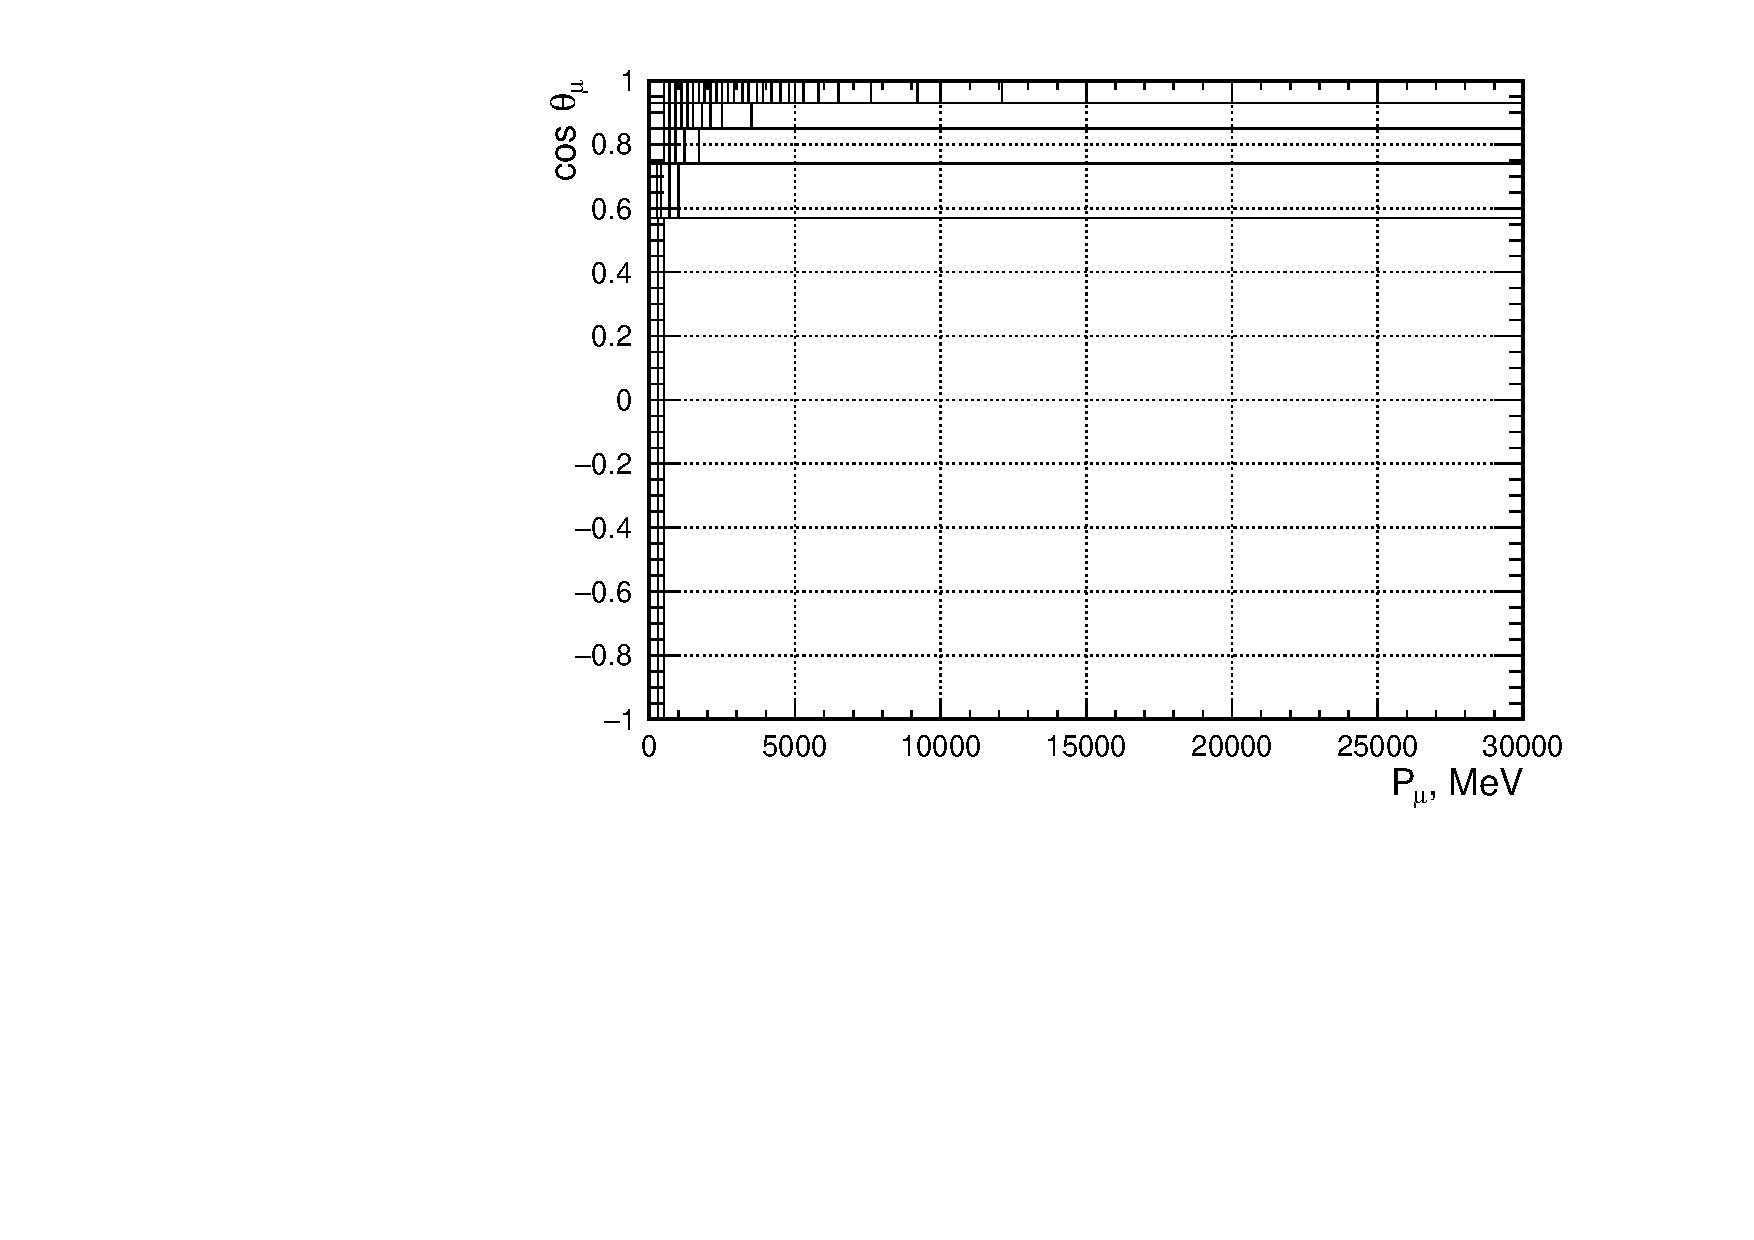
\includegraphics[width=0.95\linewidth]{figs/TH2PolyReset_MC_FGD2_NuMuBkg_CC1pi_in_AntiNu_Mode}
  \caption{FGD2 RHC $\nu_{\mu}$ 1$\pi$}
  \label{fig:TH2Poly_ResetFGD2_NuMuBkg_CC1pi_in_AntiNu_Mode}
\end{subfigure}
\begin{subfigure}{.32\textwidth}
  \centering
  \includegraphics[width=0.95\linewidth]{figs/TH2PolyReset_MC_FGD2_NuMuBkg_CCOther_in_AntiNu_Mode}
  \caption{FGD2 RHC $\nu_{\mu}$ Other}
  \label{fig:TH2Poly_ResetFGD2_NuMuBkg_CCOther_in_AntiNu_Mode}
\end{subfigure}
\caption{Non-uniform rectangular binning used in this analysis for each sample.}
\label{fig:th2polybinreset}
\end{figure}

\newpage